\chapter{A rede que Fábio e Cláudio construíram}
\label{capitulo3}

\epigrafe{%
Terceiro princípio: Nunca somos postos diante da ciência, da tecnologia e da sociedade, mas sim diante de uma gama de associações mais fracas e mais fortes, portanto, entender o que são fatos e máquinas é o mesmo que entender o que as pessoas são.}%
{Bruno Latour, \textit{Ciência em ação: como seguir cientistas e engenheiros sociedade afora}, 2011, p.~409}

Este capítulo é uma das quatro tramas da tecnoetnografia que desenvolvo nesta tese, o conceito que apresentei no capítulo~\ref{capitulo1} para nomear a indissociabilidade entre a escrita, a análise e as técnicas com que faço esta pesquisa sobre e com inteligência artificial. Se no capítulo~\ref{capitulo1} a tecnoetnografia se fez como gesto recursivo sobre a descrição etnográfica da tecnociência e seus limites, aqui ela se faz ao seguir as associações de Fábio e de Cláudio até as corporações, os contratos, as políticas de inovação e a trajetória da própria \texttt{IBM}, que recua mais de um século. Seguir essas associações é o que me impede de tomar a ciência, a tecnologia e a sociedade como três domínios já dados, postos diante de mim como blocos a relacionar; o que encontro no campo, e o que descrevo, é uma \enquote{gama de associações mais fracas e mais fortes}, em que descrever o que os contratos, as infraestruturas e as máquinas de Hollerith são não se separa de descrever o que vêm a ser os atores que se associam a eles, pois uns e outros só ganham seus contornos na trama dessas associações. A rede que descrevo neste capítulo, a dos contratos, das infraestruturas, das políticas de fomento e da trajetória corporativa, é a mesma rede sociotécnica que o capítulo~\ref{capitulo4} deixará recuar ao \textit{hinterland}, no sentido de \textcite[pp.~34--42]{Law2004After}, quando a atenção se voltar para as práticas situadas de Marcelo em torno do \texttt{Spira}, sem que essa rede de fundo desapareça, pois ela continua sendo condição de possibilidade do que aparece em primeiro plano. O que distingue este capítulo do capítulo~\ref{capitulo4} está no segmento da mesma rede que escolho seguir e no lugar onde decido começar e parar: aqui acompanho uma cadeia que se estende por muitos nós e por mais de um século; lá, Marcelo me levará a um segmento curto, em que as associações se atam mais intensamente umas às outras. Nenhum dos dois segmentos é maior ou menor que o outro, apenas mais ou menos longo, mais ou menos intensamente conectado, na formulação de \textcite{latour1996clarifications} que retomei do capítulo~\ref{capitulo1}, e o corte que decide por onde a rede se deixa rastrear é o que a faz existir como objeto etnográfico, no sentido que tomei de Strathern \parencite{strathern2011cortando}.\footnote{Latour formula a recusa das separações herdadas em dois registros que retomo ao longo deste capítulo. Na epígrafe, retirada de \textcite[p.~409]{Latour2011CienciaEmAcao}, o terceiro princípio recusa a tripartição entre ciência, tecnologia e sociedade e sustenta que só há uma gama de associações mais fracas e mais fortes, de modo que entender o que são os fatos e as máquinas se confunde com entender o que vêm a ser as pessoas. No texto sobre as propriedades da rede, Latour recusa as três dimensões espaciais herdadas das ciências sociais, a escala (grande e pequeno), a distância (perto e longe) e o limite (dentro e fora), e mostra que uma rede nunca é maior que outra, apenas mais longa ou mais intensamente conectada \parencite{latour1996clarifications}. Os dois registros convergem na mesma tese: a força e a fraqueza, o comprimento e a intensidade da conexão são graus de um único contínuo de associações, e não propriedades de domínios ou de escalas distintas. É por isso que a diferença entre este capítulo e o capítulo~\ref{capitulo4} se decide no corte que faço sobre a mesma rede, no sentido de \textcite{strathern2011cortando}, e não em uma diferença de natureza entre duas redes.}

Segui Fábio e Cláudio presencialmente, ao longo dos eventos, das conversas e das reuniões em que os encontrei, durante aproximadamente quatro anos de pesquisa etnográfica (2022--2025) no \texttt{C4AI}. O trabalho de campo intensificou-se a partir de fevereiro de 2023, quando assisti à \textit{bluetalks} (encontro corporativo para discutir tecnologia e inovação) realizada no Inovabra Habitat em São Paulo,\footnote{O Inovabra é um espaço de inovação criado pelo banco Bradesco, situado na região da Avenida Paulista, em São Paulo, que aproxima \textit{startups}, empresas, mentores e investidores. O evento ocorreu poucos meses antes de a Organização Mundial da Saúde declarar, em maio de 2023, o fim da emergência de saúde pública internacional da Covid-19.} evento em torno do qual se organizou a problematização que deu origem a este capítulo. Numa quinta-feira de fevereiro, eu era parte da audiência quando uma pessoa da plateia, uma mulher cujo nome não registrei, perguntou a Cláudio, vice-diretor do \texttt{C4AI} e à época ainda pesquisador da \texttt{IBM}, o que a \texttt{IBM} ganhava com o investimento no centro. Cláudio respondeu que a empresa se beneficiava ao \enquote{incentivar um ecossistema de inovação em inteligência artificial} para que as pesquisas atendessem às necessidades do setor, de modo que surgiria \enquote{uma demanda por serviços que a IBM poderia fornecer}. Foi essa resposta, dada naquelas condições, que me deteve. Embora circule amplamente a percepção de que empresas buscam extrair valor de suas parcerias, poucas vezes se descreve o que de fato circula nessas cadeias, por quais caminhos e sob que termos, e foi essa a lacuna que tomei como questão. Não tomo a resposta de Cláudio como descrição verificada do que a \texttt{IBM} ganha, e não disponho de meios para saber se o retorno que ele antecipava chegou a se confirmar; o encerramento posterior da operação da empresa no Brasil, que ultrapassa o \texttt{C4AI} e ao qual retorno ao fim deste capítulo, deixa a questão em aberto. A fala abriu a pergunta que eu viria a perseguir, a de como circula o valor nessas cadeias, e foi ao perseguir o que ela significava que entendi o que era seguir Fábio e Cláudio: acompanhar as associações que eles faziam e, ao mesmo tempo, fazer associações eu própria ao segui-los, de modo que eu também entrava na rede que descrevia.

Foi também assim que cheguei à \texttt{IBM} como objeto de pesquisa. Até então, a empresa era um ator coadjuvante que ora aparecia, ora recuava, e como investigar o convênio público-privado em si não estava entre minhas intenções, eu nunca lhe havia dado a atenção que ela merecia. Ao perseguir o que a resposta de Cláudio significava, a \texttt{IBM} deixou de ser figura de fundo e passou a ocupar o centro desta investigação, num deslocamento metodológico que mudou o foco de uma etnografia do presente, de como se faz pesquisa em IA no \texttt{C4AI}, para uma investigação histórica que relaciona este centro a práticas tecnocientíficas estabilizadas pela \texttt{IBM} ao longo de mais de um século. Tomá-la como objeto e levar essa análise adiante tensionou a minha posição de pesquisadora, e foi por meio dela que experimentei, na própria prática, o esforço de fazer alianças sem ferir os sentimentos estabelecidos, no sentido de Stengers, que abordei no capítulo~\ref{capitulo1}. Como viria a descobrir, esta etnografia tornou-se também um registro, ou uma reconstrução, da trajetória do acordo \texttt{C4AI-IBM-FAPESP}, desde a sua criação em 2020, passando por sua relativa consolidação e multiplicação institucional, até o seu encerramento pela \texttt{IBM} em dezembro de 2025. O que começou como tentativa de compreender como se faz IA em um centro de pesquisa transformou-se, por força do próprio campo, em documentação de como arranjos desse tipo se formam, funcionam e acabam, e de como relações de poder, o \textit{tecnopoder} que proponho nomear adiante, mostram-se em momentos de tensão, de crise e de êxito, revelando negociações nem sempre explícitas entre atores e actantes que transitam entre discursos sobre \enquote{IA responsável}, \enquote{bem social} e \enquote{mercado}. Essas racionalidades corporativas continuam a influenciar relações entre corporações globais e instituições acadêmicas que, embora robustas em seus contextos nacionais, ocupam posição periférica nos ecossistemas globais de inovação em inteligência artificial, ecossistemas que influenciam, e até mesmo determinam, quem pode fazer IA, como fazer, para quê e para quem.

À fala da \textit{bluetalks} soma-se uma segunda, que Cláudio me deu em entrevista realizada em 2025, e os dois são fios distintos que costuro ao longo desta trama: o primeiro diz respeito ao que a \texttt{IBM} ganha ao cultivar um ecossistema de pesquisa em torno de si, e o segundo, ao modelo de negócio que a empresa montou sobre o código aberto. Aproximá-los não os torna a mesma coisa, e é a relação entre eles que a investigação histórica deste capítulo procura descrever. Referindo-se a esse modelo de negócio, Cláudio mencionou que a \texttt{IBM} \enquote{descobriu na década de 90} como fazer dinheiro com \texttt{Linux} e sistemas abertos (\textit{open source}). Chamou-me a atenção a escolha do verbo: \enquote{descobriu}, e não \enquote{desenvolveu} ou \enquote{inventou}. Leio nessa escolha um indício de que se trata, para ele, de uma prática que a \texttt{IBM} encontrou já formada e passou a explorar, em lugar de algo que ela teria criado, e é essa leitura que a investigação histórica deste capítulo desenvolve.

Foi seguir o que \textit{descobriu} implicava que me levou a investigar o que o código aberto tinha a ver com o \texttt{C4AI} e com os ecossistemas de inovação em IA. O paralelo com a inteligência artificial contemporânea é de longa duração: assim como o modelo de negócios de código aberto permitiu que corporações extraíssem valor gerado coletivamente por comunidades de desenvolvedores, os atuais modelos de IA dependem da extração e do processamento de conhecimento produzido coletivamente, seja por meio de dados gerados por usuários, cuja origem se torna difícil de rastrear na escala em que esses sistemas funcionam,\footnote{Se o caso do \texttt{GitHub Copilot} expõe o corte da propriedade no plano do código, os dados de treinamento o expõem em outra escala. A auditoria de \textcite{Longpre2024Provenance} sobre quase quatro mil conjuntos de dados públicos de texto, fala e vídeo, produzidos entre 1990 e 2024, precisou rastrear manualmente cada conjunto até suas fontes originais, percorrendo cadeias de repositórios, sites e artigos, porque a documentação de proveniência se perde a cada vez que um conjunto é reempacotado e re-licenciado. Os autores constatam que, embora menos de um terço dos conjuntos tenha licença restritiva, mais de 80\% do conteúdo de suas fontes carrega restrições não declaradas na licença final, e que a licença do conjunto contradiz os termos da fonte em mais da metade do conteúdo de texto. O rastreamento foi possível para os auditores, ao custo de um trabalho manual extenso, mas não está documentado para quem usa esses conjuntos nem para quem teve seus dados incorporados a eles: a origem é conhecida por quem coleta e se apaga para quem contribuiu. A irrastreabilidade, no caso da IA, distribui-se de modo desigual entre os lados da rede.} seja pelos vínculos com universidades públicas que fornecem pesquisadores, infraestrutura e legitimidade epistêmica.\footnote{Desenvolvo essa literatura crítica da extração algorítmica e da inteligência artificial no capítulo~\ref{capitulo2} (seção~\ref{sec:predicao_poder}), a propósito de Kate Crawford, Vladan Joler e Matteo Pasquinelli: as cartografias que seguem as cadeias materiais, laborais e epistêmicas da IA, e o argumento de que esses sistemas atualizam padrões de longa duração de colonialismo e extração.} O caso do \texttt{Linux} evidencia, historicamente, a apropriação corporativa do conhecimento coletivo na indústria de tecnologia. Trata-se de um modelo que funciona simultaneamente em dois registros: produz bens públicos (código aberto, modelos de IA, publicações científicas) enquanto gera lucro privado (serviços, consultorias, infraestrutura proprietária). Bem público, porém, não é o mesmo que bem social: um sistema de IA pode ser tecnicamente \enquote{aberto} e ainda assim aprofundar desigualdades e favorecer infraestruturas proprietárias. Os recursos que utilizei para as análises computacionais desta tese são um exemplo de como isso funciona na prática: hospedo no \texttt{GitHub} os repositórios públicos desta pesquisa, da análise lexicométrica ao código-fonte do texto. A mesma abertura que torna o meu trabalho verificável, auditável e reexecutável o disponibiliza como código público a quem treina modelos sobre esses acervos.\footnote{A \texttt{Microsoft} comprou o \texttt{GitHub}, plataforma que hospeda boa parte do desenvolvimento de código aberto do mundo, em 2018, por US\$ 7,5 bilhões \parencite{Microsoft2018GitHub}; em 2021, o \texttt{GitHub Copilot}, assistente de programação movido pelo modelo \texttt{Codex} da \texttt{OpenAI}, foi lançado treinado sobre bilhões de linhas de código público hospedado na própria plataforma, sem a atribuição de autoria que as licenças \textit{open source} exigem, o que motivou uma ação coletiva contra \texttt{GitHub}, \texttt{Microsoft} e \texttt{OpenAI} em 2022.}

O termo \textit{tecnopoder} deriva da noção de \enquote{poder artificial} (\textit{Artificial Power}) com que \textcite{Brennan2025ArtificialPower} sintetizam o contexto em que uma \enquote{oligarquia tecnológica} mobiliza a IA, como uma categoria de marketing e como conjunto de tecnologias de automação, para consolidar e ampliar o seu poder. Tomo esse termo emprestado e o desloco para o meu material, para investigar práticas tecnocientíficas da \texttt{IBM} ao longo de 135 anos, dos cartões perfurados de Hollerith às plataformas de IA contemporâneas. A derivação é também conceitual: o que muda é o estatuto que cada abordagem confere à desigualdade de poder. Para a literatura crítica das \textit{big techs}, que pensa a IA como concentração de poder, essa desigualdade é o que explica os arranjos concretos; para a teoria ator-rede que sigo, ela é o efeito que precisa ser descrito, rastreado associação por associação até os mecanismos que o produzem, e não a causa que explica. Mantenho as duas formas de investigação em tensão: recorro à teoria ator-rede para descrever como as desigualdades se fazem, relação por relação, e ao vocabulário da crítica para nomear o padrão histórico desse contexto, ciente de que esse vocabulário, com termos como captura, dependência e extração, carrega pressupostos sobre estruturas tecnocientíficas geralmente problemáticos para o escopo da teoria ator-rede. É dessa tensão que extraio o método: a descrição actante a actante me impede de tomar a desigualdade como causa já pronta, e o vocabulário da crítica me impede de dissolver, na simetria descritiva, a desigualdade de poder que o campo me apresentou. É nesse intervalo que situo o \textit{tecnopoder}.

Cheguei à \texttt{IBM}, portanto, seguindo as falas públicas de Fábio e de Cláudio, e a pergunta que alguém da plateia da \textit{bluetalks} dirigiu a Cláudio, e com ela a um sistema de tabulação, a máquina tabuladora que Herman Hollerith (1860--1929) criou nos finais do século XIX. Embora este seja o terceiro capítulo na ordem em que a tese se lê, foi a \texttt{IBM} o primeiro dos sítios que segui a se impor à investigação, e marco essa diferença porque foi seguir os atores que decidiu por onde a pesquisa começaria a se adensar. O lugar que a empresa veio a ocupar na pesquisa contrariou o que eu esperava. Eu entrara em campo determinada a fazer uma etnografia mais voltada aos actantes não humanos, os sistemas de IA do centro, que aos atores, os cientistas e engenheiros, e contava encontrar um laboratório de pesquisa em IA onde observaria de perto como se faz inteligência artificial. O laboratório que eu imaginava não estava lá. Foi a frustração dessa expectativa, que no capítulo~\ref{capitulo1} formulei como a pergunta \emph{onde está o laboratório e os seus cientistas?} (seção~\ref{onde-esta-laboratorio-cientistas}), que me levou, primeiro, à \texttt{IBM} e a Hollerith: é aqui, nesta rede, que aquela pergunta que abri no início desta tese ganhou contornos próprios. O conselho de Latour para suspender preconceitos e expectativas ao entrar no mundo da ciência e da tecnologia valeu-se nesse ponto, quando a expectativa frustrada se tornou uma condição de realização desta etnografia.\footnote{\enquote{O equipamento necessário para viajar pela ciência e pela tecnologia é, ao mesmo tempo, leve e variado. Variado porque é preciso misturar pontes de hidrogênio com prazos finais, exame da capacidade alheia com dinheiro, correção de sistemas de computadores com estilo burocrático; mas o equipamento também é leve porque convém deixar de lado todos os preconceitos sobre as distinções entre o contexto em que o saber está inserido e o próprio saber. Na entrada do inferno de Dante está escrito: DEIXAI A ESPERANÇA, Ó VÓS QUE ENTRAIS. No ponto de partida desta viagem deveria estar escrito: DEIXAI O SABER SOBRE O SABER, Ó VÓS QUE ENTRAIS.}\parencite[p.~10]{Latour2011CienciaEmAcao}.}

\section{Do C4AI-IBM à Terra}
\label{sec:cadeia_translacao}

A Figura~\ref{fig:texto-mapa-cap3} constitui um texto-mapa em que o percurso do capítulo se distribui em uma superfície cuja leitura faço em etapas: parto da pergunta que o campo me deu, sigo pelos fios que dela se desdobram até as máquinas de Hollerith, e chego, por fim, ao arremate que reabre a questão sobre a universidade. O capítulo inicia com a decisão de seguir Fábio e Cláudio, abre a pergunta histórica sobre o ecossistema de inovação, reconstrói a trajetória da \texttt{IBM} de Hollerith ao \texttt{C4AI}, mostra o que as entrevistas tornaram dizível, incluindo a análise bibliométrica das publicações do centro, e lê o fim da parceria como o evento que torna legíveis as ausências que o arranjo não inscreveu, para então devolver, nas considerações finais, a pergunta sobre o lugar da universidade na pesquisa em IA.

\begin{figure}[!htb]
  \centering
  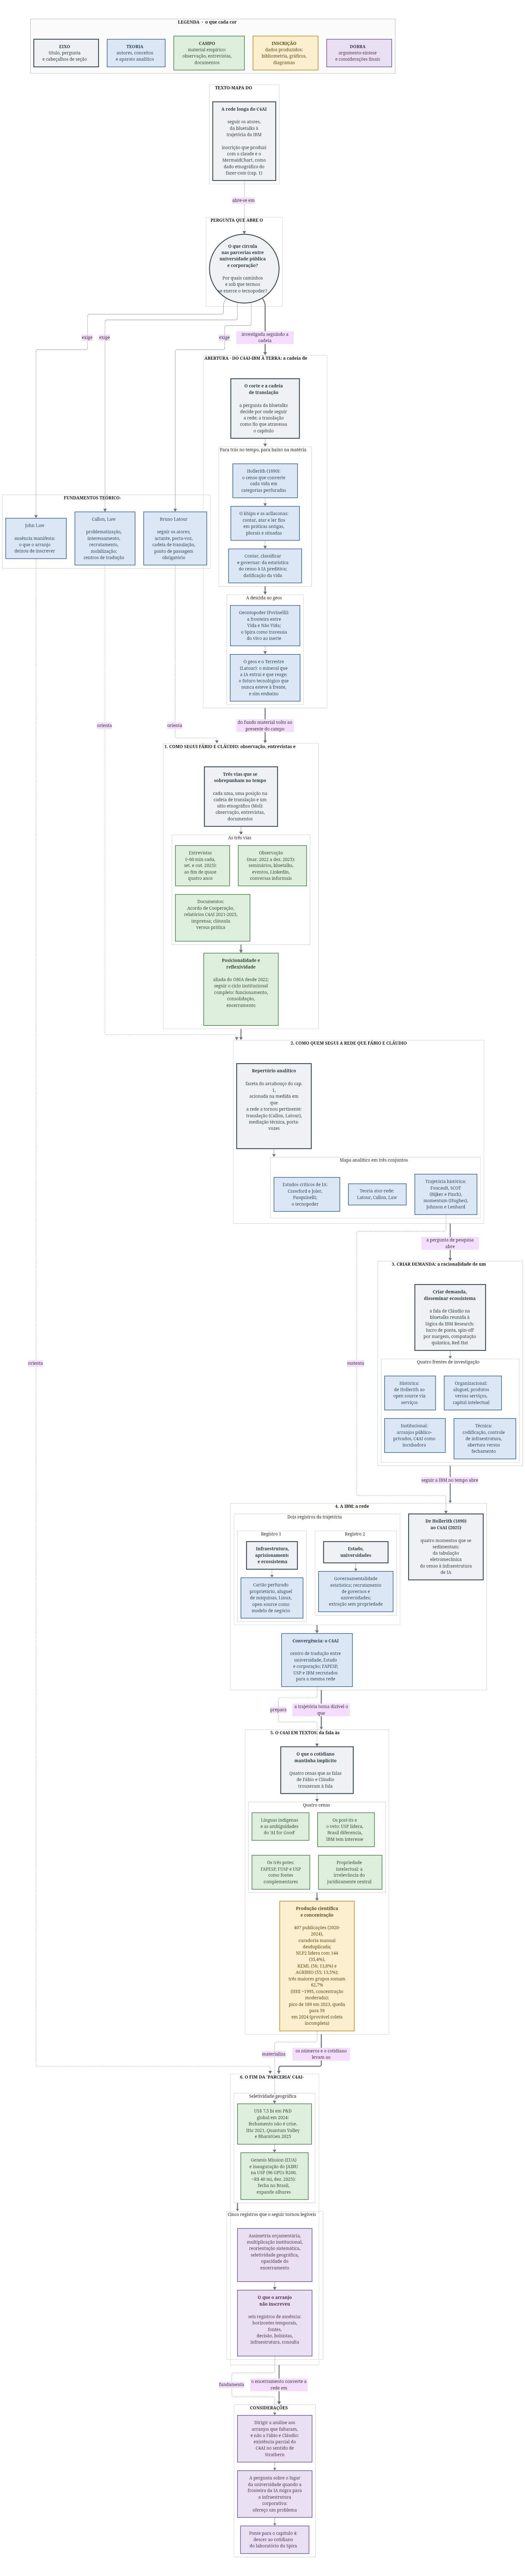
\includegraphics[width=0.2\textwidth,keepaspectratio]{figuras/cap.3/diagramas/mapa-capitulo3.png}
  \caption[Texto-mapa do capítulo~\ref{capitulo3}]{\textbf{Texto-mapa do capítulo~\ref{capitulo3}: a rede longa do \texttt{C4AI}, dos porta-vozes à trajetória da \texttt{IBM}.} A inscrição dispõe o percurso do capítulo a partir da pergunta que o campo me devolveu, sobre o que circula nas parcerias entre universidade pública e corporação, por quais caminhos e sob que termos se exerce o tecnopoder. Três fundamentos sustentam o percurso: \textcite{Latour2011CienciaEmAcao} (seguir os atores), \textcite{Callon1986Sociology} (problematização, interessamento, recrutamento e mobilização) e \textcite{Law2004After} (a ausência manifesta, o que o arranjo deixou de inscrever). (i)~Em \textit{Do C4AI-IBM à Terra}, parto da pergunta que o campo me devolveu e sigo a cadeia de translação para trás no tempo, da parceria à tabulação de Hollerith e ao \textit{khipu}, e para baixo na matéria, até o mineral e a Terra de que a inteligência artificial nunca se desprende. (ii)~Em \textit{Seguindo Fábio e Cláudio: observação, entrevistas e documentos}, o deslocamento de uma etnografia do fazer IA para uma etnografia do arranjo que torna esse fazer possível, ativado pela agência da \textit{bluetalks} de fevereiro de 2023, mobiliza o mapa analítico em três conjuntos (teoria ator-rede; trajetória histórica com Foucault, a SCOT de Bijker e Pinch e o \textit{momentum} de Hughes; estudos críticos de IA com Crawford, Joler e Pasquinelli). (iii)~Em \textit{\enquote{Criar demanda}: a racionalidade de um ecossistema}, a fala de Cláudio na \textit{bluetalks} reúne-se à lógica da \texttt{IBM} Research e abre as quatro frentes da pergunta histórica, da tabulação ao \textit{open source} via serviços. (iv)~Em \textit{A trajetória da \texttt{IBM}}, a rede longa de Hollerith (1890) ao \texttt{C4AI} desdobra-se em dois registros, a infraestrutura e o aprisionamento por ecossistema e a captura epistêmica do Estado e das universidades, que convergem no \texttt{C4AI} como centro de tradução. (v)~Em \textit{As entrevistas com Fábio e Cláudio}, quatro cenas que o cotidiano mantinha implícitas (o \textit{Design Thinking} e o veto corporativo, os três potes do financiamento, a propriedade intelectual e as ambiguidades do \textit{AI for Good}) levam à análise bibliométrica das publicações do centro. (vi)~Em \textit{O fim da \enquote{parceria} \texttt{C4AI-IBM}}, a seletividade geográfica dos investimentos da \texttt{IBM} e os cinco registros que emergiram do seguir dos atores levam aos seis registros de ausência, o que o arranjo não inscreveu. As considerações finais dirigem a análise aos arranjos que faltaram, devolvem a pergunta sobre o lugar da universidade e fazem a ponte para o capítulo~\ref{capitulo4}. Versão interativa disponível em \url{https://mermaid.ai/d/0c8eb50f-d995-4bba-b60a-c768ebe5dd51}.}
  \label{fig:texto-mapa-cap3}
\end{figure}

Esta investigação, que se intensifica a partir de uma rápida conversa num auditório de banco em São Paulo e recua até a máquina de tabular cartões perfurados de 1890 nos Estados Unidos, foi o que significou, neste capítulo, \enquote{seguir os atores}: seguir o fio da conversa que Fábio e Cláudio iam tecendo quando se referiam a noções como \enquote{ecossistema de inovação} e \enquote{criação de demanda}, ou ao modo como a \texttt{IBM} \enquote{descobriu nos anos 90} a possibilidade de lucrar com código aberto. Associação por associação, surgiam questões que me fizeram voltar ao tempo e perguntar: por quais modos uma corporação passa a extrair valor de suas conexões com universidades? O que significa \enquote{fortalecer um ecossistema de IA}? De que maneira se \enquote{descobre} um modelo de negócios baseado em código aberto, e como essa descoberta passa a orientar políticas tecnocientíficas globais de empresas de alta tecnologia? E como tudo isso se relaciona com um centro de IA em uma universidade pública brasileira? Trago essas perguntas porque foram elas o material que pôs o pensamento em movimento. Algumas se desdobraram na trajetória histórica que reconstruo a seguir, outras permaneceram abertas, e é desse desdobramento que se faz a trama deste capítulo.

Como discuti no capítulo~\ref{capitulo1}, subseção~\ref{subsec:cortando-redes}, seguir cientistas e engenheiros universidade afora implicou atravessar fronteiras disciplinares, temporais e geográficas e, sobretudo, manter-me \enquote{tão indecisa quanto os diversos atores que seguia}, ou seja, retomando a epígrafe que abre este capítulo, resistir à tendência de separar o \enquote{técnico} do \enquote{social}, o \enquote{interno} do \enquote{externo}, o \enquote{científico} do \enquote{comercial}. A escolha de quem seguir, porém, foi decidida. Comecei por Fábio e Cláudio porque eram quem mais se sobressaía no campo naquele momento da pesquisa, falando do centro em toda parte, à frente de um arranjo em consolidação e em busca de aliados, e foi a essa proeminência que respondi quando os escolhi como atores a seguir, na seleção das entrevistas que descrevo no capítulo~\ref{capitulo1}, subseção~\ref{subsec:corte_reflexivo_cap1}. Que eles falavam em nome do \texttt{C4AI}, eu viria a descrevê-los como porta-vozes, no sentido que assento adiante; no instante da escolha, porém, o que se impôs foi essa presença proeminente. Os caminhos que essa escolha abriu, fui-os fazendo conforme as associações se desenrolavam, de modo que eu não dispunha, de antemão, de onde a rede que eles construíam começava nem de onde eu poderia cortá-la. Quem eu seguia hoje me apontava para quem eu seguiria amanhã, e cada ator que se somava à rede reabria a pergunta sobre os seus limites. Assim, fui fazendo o caminho a cada associação, retomando a epígrafe que abre esta tese: \enquote{Caminante, no hay camino,\slash{} se hace camino al andar} \parencite[p.~88]{machado2005campos}. E foi esse caminhar, feito e refeito a cada associação que se revelava, que me levou à \textit{bluetalks}. Tivesse eu separado de antemão o \enquote{acadêmico} do \enquote{corporativo}, teria tratado a \textit{bluetalks} como evento de negócios alheio ao meu campo e não teria ido até lá; e, faltando essa ida, faltaria também a conversa entre Cláudio e a audiência; aprendi ali, e por isso, que aquele tipo de encontro também era uma forma de fazer tecnociência, e, naquele caso, de fazer pesquisa em IA.

Olhando para trás, aquela pergunta da plateia, ou melhor, o conjunto de questões que ela abriu, indicou onde eu cortaria a rede, no sentido que tomei de Strathern \parencite{strathern2011cortando}. O corte foi o gesto que fez a rede aparecer como objeto a seguir, mais do que uma subtração que deixasse um pedaço de fora. Esses cortes costumam ser feitos quase que intuitivamente, e foi por isso que me voltei a este como um elemento etnográfico que importa para esta tese: foi uma pergunta dirigida a Cláudio que apontou por onde eu iria para construir essa rede junto a ele e a Fábio. Descrevê-la como corte foi o que me afastou de tomá-la por uma hipótese de pesquisa a confirmar. O ponto em que essa pergunta incidiu me parece consequente, e é aqui que o corte e o que ele faz aparecer deixam de ser duas coisas. Ao perguntar o que a \texttt{IBM} ganha, a pergunta tocou no que Strathern analisa a partir do conceito de \emph{propriedade} em \enquote{Cortando a Rede}, como uma relação que corta, isto é, o gesto que destaca algo do fluxo das transferências e o fixa como pertencente a alguém, ali onde de outro modo continuaria a circular \parencite[p. 29]{strathern2011cortando}. Discuto esse corte no capítulo~\ref{capitulo1}. Strathern parte do caso da patente do vírus da hepatite C, na qual a rede dos cientistas que tornaram a descoberta possível é truncada no instante em que a propriedade decide qual segmento dela pode ser reivindicado, separando quem pertence de quem não pertence \parencite[pp. 27--29]{strathern2011cortando}. Com essa mesma ideia, em \textit{Property, Substance and Effect}, Strathern descreve como as cadeias longas de intercâmbio de conhecimento que levam a uma invenção comercializável se rompem em segmentos no momento em que se requer a patente, e como as práticas ditas \enquote{colaborativas} encobrem as próprias linhas de exploração que as atravessam \parencite[p.~169]{strathern2000pse}. A pergunta vinda da plateia atravessou a rede porque incidiu justamente no ponto em que se define a propriedade, isto é, no gesto de separar o que pertence a cada um, o que se extrai de quem, o que se retém e o que se deixa escapar. No caso da inteligência artificial, esse mesmo corte torna-se mais difícil de identificar, pois, enquanto a patente examinada por Strathern interrompia uma rede de pesquisadores nomeáveis, o treinamento de modelos se apoia em uma multidão de contribuições cuja procedência é conhecida por quem coleta, mas se obscurece para quem contribuiu, como argumentei no início deste capítulo ao tratar do código aberto e dos dados de treinamento.

Assim, o corte decidiu por onde eu seguiria a rede neste capítulo. Foi, a partir disso, que voltei à pergunta que situa a questão de pesquisa desta tese, a de onde estavam o laboratório e os seus cientistas, e o que ela encontrou aqui foi um \enquote{laboratório distribuído}, espalhado por muitos lugares no tempo e no espaço, no lugar do espaço único onde eu esperava ver os cientistas e engenheiros fazendo IA.\footnote{A configuração distribuída do \texttt{C4AI} antecede a pandemia, por ser parte do modelo CPE-Fapesp, mas as restrições sanitárias de 2020-2023 a intensificaram, como detalho adiante. Diana Forsythe, em suas etnografias de laboratórios de IA das décadas de 1980-90, sustenta que a opacidade do \enquote{fazer IA} é dimensão constitutiva do campo, com atenção ao modo como certos trabalhos, de anotação, de manutenção, de tradução entre especialistas e leigos, desaparecem das narrativas oficiais da ciência, no gesto que ela nomeia \textit{deletion of work} \parencite{Forsythe2001}. Tomo a formulação de Forsythe como referência para o que encontrei no \texttt{C4AI}, sem decidir, a partir do meu material, se a opacidade que descrevo confirma essa tese ou tem raízes próprias na configuração do Centro, questão que retomo adiante.} Foi essa dispersão, no lugar do laboratório que eu imaginava, que o próprio campo me deu a seguir, e que encaminhou a investigação para as questões de governança, dependência tecnológica e extração de valor que ocupam este capítulo; o feitio etnográfico permaneceu, ainda que escapasse ao que eu havia imaginado, e esse escape provou-se constitutivo da prerrogativa de seguir os atores. Para dar conta dessas questões, fui articulando os referenciais à medida que as associações se desdobravam e eu precisava descrevê-las, conforme discuto no capítulo~\ref{capitulo2}.

Nesse sentido, o conceito de \textit{cadeia de translação} atravessa toda a tese, e acompanha o modo como atores e actantes recrutam aliados, fixam pontos de passagem e fazem associações que perduram no tempo e no espaço. Assentei o conceito de \textit{translação} no capítulo~\ref{capitulo2}, ao separar as duas acepções que Callon e Latour lhe deram. Callon a desdobra em quatro momentos e descreve como os actantes se alistam; Latour a toma como o primeiro dos quatro sentidos da mediação técnica e descreve o que sobrevém aos objetivos de cada um no instante do alistamento. Ao tratar da mediação, lá, segui Latour e os seus quatro sentidos; aqui, acresço Callon, cujos próprios objetos de pesquisa guardam afinidade maior com a análise que faço neste capítulo. Foi Callon que investigou redes que articulam um polo científico, um polo técnico e um polo de mercado, e nelas as empresas que se fazem ponto de passagem, o financiamento que se traduz em programa de ação e a convergência que, ao endurecer, torna-se irreversível.\footnote{\textcite{Callon1991Techno} chama essas redes de tecnoeconômicas e mostra como nelas humanos e não humanos, inscrições e dinheiro se associam em torno dos três polos; o alinhamento e a coordenação dessas associações é o que mede a sua convergência, e a sua irreversibilização é o que faz uma translação perdurar e predeterminar as seguintes.} Foi mais ou menos isso que encontrei ao seguir Fábio e Cláudio a recrutar aliados e a \texttt{IBM} a fazer-se ponto de passagem, e nos quatro momentos da translação achei o fio com que descrever essa rede.\footnote{\textcite{Callon1986Sociology} desdobra a translação em quatro momentos, a problematização, o interessamento, o recrutamento e a mobilização, pelos quais um actante se faz porta-voz de outros e desloca os interesses de cada um para um ponto de passagem comum. \textcite{Latour2011CienciaEmAcao} e \textcite{Latour2017Esperanca} tomam o conceito para descrever o que sobrevém aos objetos ao longo da cadeia: cada etapa transforma e desloca o que recebe, e o objeto que chega ao fim não é o que partiu do início. No capítulo~\ref{capitulo4}, é Latour quem predomina, porque ali sigo os objetos, e não os atores, ao longo da cadeia de inscrições. Cada capítulo se lê por si: as remissões entre eles servem de baliza, não de pré-requisito.}

Voltei à \texttt{IBM} porque é nela que essa cadeia de translações ganha espessura histórica. Antes da máquina, quem computava era gente: equipes de calculadores humanos, em sua maioria mulheres, somavam e tabulavam à mão os números do mundo. A máquina de Herman Hollerith, montada para a realização do primeiro censo estadunidense demográfico automatizado em 1890, deslocou esse trabalho para o cartão perfurado e o cartão para a leitora eletromecânica, e foi a primeira a fazê-lo na escala de uma população inteira. Da Tabulating Machine Company de Hollerith descende, por fusões sucessivas, a \texttt{IBM}, que herdou esse sistema de tabulação e o levou adiante, do eletromecânico ao eletrônico das válvulas, do transistor ao circuito integrado, da integração em larga escala do \textit{chip} à nuvem e à inteligência artificial. A \texttt{IBM} é um nó desta tese porque atravessou todas essas passagens e, ao lado de outras corporações de tecnologia, ajudou a movê-las, e porque foi a empresa que industrializou a primeira dessas camadas, a tabulação mecânica, e a pôs a contar populações.\footnote{Reconstruo essa trajetória a partir de \textcite{Austrian1982Hollerith} sobre Hollerith e a invenção da tabulação mecânica, \textcite{Pugh1995Building} sobre a \texttt{IBM} e seus primeiros computadores, e \textcite{Cortada2019IBM} sobre a trajetória corporativa da empresa. A \texttt{IBM} não existia em 1890: a máquina é de Hollerith e de sua Tabulating Machine Company, fundada em 1896, que se funde a outras duas na CTR de Charles Flint em 1911 e só toma o nome International Business Machines em 1924. Quando digo que a \texttt{IBM} industrializou a tabulação mecânica, falo dessa linhagem, e a desdobro nos quatro momentos da seção~\ref{subsec:registro2}.}

\begin{figure}[htbp]
  \centering
  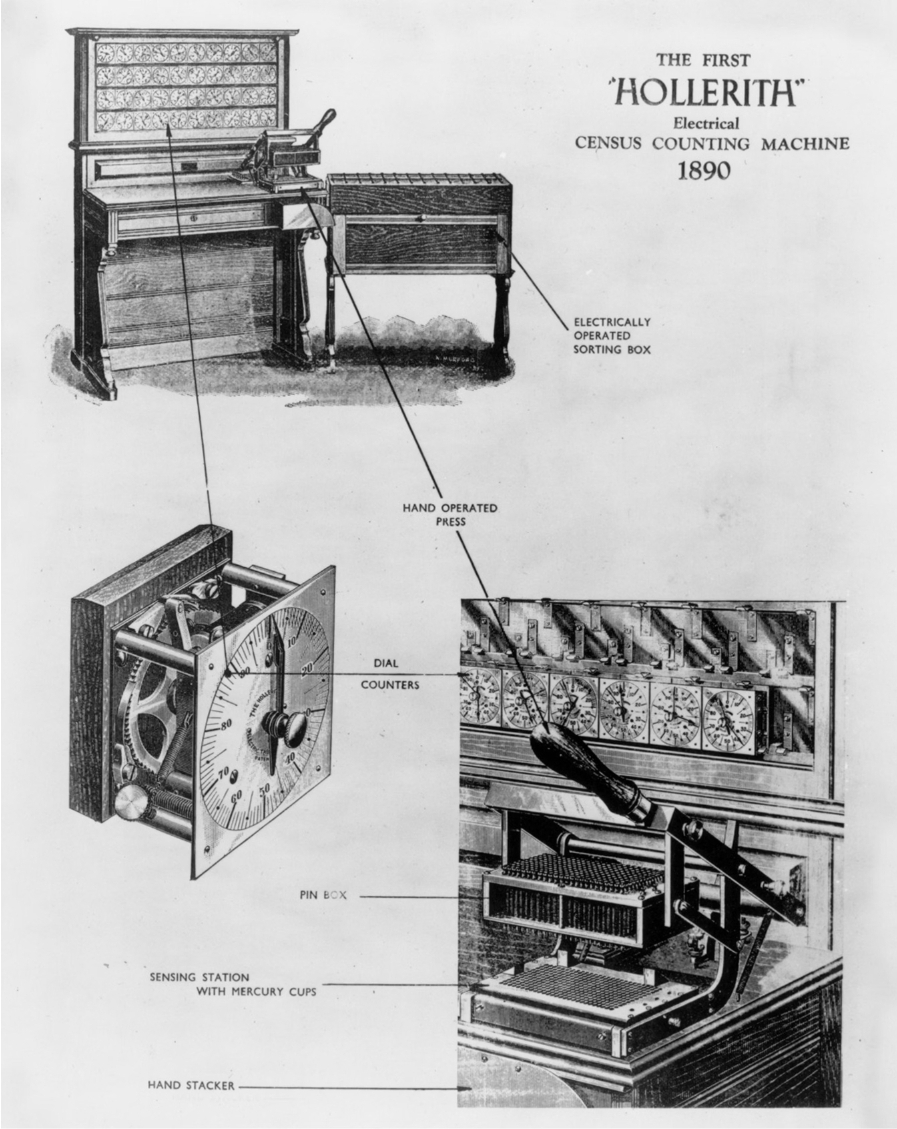
\includegraphics[width=0.6\textwidth]{figuras/cap.3/hollerith_1890_product_sheet.png}
  \caption[Folha de produto da máquina de tabulação de Hollerith (1890)]{Folha de produto de 1890 anunciando \enquote{The First Hollerith Electrical Census Counting Machine}, a máquina eletromecânica de tabulação por cartões perfurados empregada no censo estadunidense de 1890.} 
  \label{fig:maquina_hollerith}
  \fonte{\textcite{IBM_HollerithTabulator}. Disponível em: \url{https://www.ibm.com/history/punched-card-tabulator}. Acesso em: \today.}
\end{figure}

Antes de seguir essa linha, detenho-me num fio que vem do capítulo~\ref{capitulo2} e que prefiro não soltar ainda. Lá rastreei, na obra de Latour, a tensão entre a figuração militar do alistamento e a figuração têxtil da trama, e sustentei, com Haraway, que importa com que figurações se pensa, porque cada uma faz aparecer um mundo e deixa outros na sombra \parencite{Haraway2023Ficar}. Levo esse cuidado comigo ao voltar-me para a história da computação que desemboca na \texttt{IBM}, porque a história que se conta com mais frequência, a que vai da máquina de Hollerith ao computador eletrônico e daí à inteligência artificial, é uma história em que computar foi, desde sempre, calcular com números e com máquinas em uma escala ascendente contínua de desenvolvimento tecnológico. Outras histórias, porém, foram tecidas com outras matérias, e uma delas me interessa de perto, porque computa com fios e nós, e porque, ao computar, também conta histórias. O \textit{khipu} andino, do quéchua \textit{khipu}, \enquote{nó}, era um aparato de cordéis atados, um cordel principal do qual pendiam cordéis secundários (Figura~\ref{fig:khipu_chancay_huando}), em que os povos dos Andes, e de modo notável o Estado inca entre cerca de 1450 e 1532, inscreviam em um só gesto o que se conta e sobre o que se conta, de um lado, censos, tributos e calendários; de outro, genealogias, feitos e histórias de pessoas, de lugares e de tempos \parencite{urton2003signs, quilter2002narrative}.\footnote{Traduzo por \enquote{cordel} o termo \textit{cord} de Urton, que nomeia tanto o cordel principal quanto os pendentes. A palavra carrega, em português, a ressonância com a literatura de cordel, e a acolho de propósito. Como o folheto pendurado em barbante, o \textit{khipu} conta e reconta, e a coincidência reforça a figuração têxtil com que penso este aparato.} Os primeiros cronistas espanhóis já notaram essa dupla natureza, ao verem os guardiões dos fios ora desatar e reatar nós para acertar as contas de um depósito, ora recitar, a partir das mesmas cordas, a memória de feitos passados \parencite[p.~67]{quilter2002narrative}. O subtítulo do volume que Jeffrey Quilter e Gary Urton organizam, \emph{accounting and recounting}, nomeia essa indistinção, e o português a aproxima mais do que o inglês, porque \enquote{contar} é ao mesmo tempo enumerar e narrar, e \enquote{conta} e \enquote{conto} partilham a raiz.\footnote{Urton mostra que a própria separação entre \textit{khipu} numérico e \textit{khipu} narrativo começa a se desfazer quando se olha de perto, porque os mesmos traços, a cor, o sentido da torção, a oposição entre o claro e o escuro, carregam ao mesmo tempo a soma e o sentido que a ordena \parencite{quilter2002narrative}.}

A estrutura dos \textit{khipus} também se fazia por um sistema binário, a direção da fiação e da torção do fio, o sentido em que o nó era atado, a cor, o número, cada traço abrindo uma escolha entre dois estados, e o conjunto deles compondo o que Urton descreve como sequências de sete dígitos binários, sete \textit{bits}, à maneira como a computação eletrônica compõe cada caractere numa sequência de \textit{bits} \parencite[pp.~1--2, 109--117]{urton2003signs}. O computador chegou à codificação binária por tentativa e erro, ao passo que o \textit{khipu} já era, por sua própria natureza, um dispositivo binário, porque a sua matéria, o fio que se fia em um sentido ou em um outro, o nó que se ata por um lado ou por outro, é feita de pares de alternativas \parencite[p.~109]{urton2003signs}. Tanto o sete do \textit{khipu} quanto o oito da computação são escolhas, e nada na lógica do dois estados obriga ao oito; ela exige apenas que cada dígito decida entre 0 e 1, e nada diz quantos dígitos reunir em uma unidade, tanto que máquinas distintas já agruparam os \textit{bits} de seis em seis, de sete em sete, de doze em doze \parencite[pp.~115--117]{urton2003signs}.\footnote{O padrão de codificação de caracteres que se tornou corrente, o \texttt{ASCII}, fixou-se em sete \textit{bits}; foi a \texttt{IBM} que estabeleceu o agrupamento de oito, o \textit{byte}, como unidade ao projetar o \texttt{System/360} em 1964, e foi pela compatibilidade que esse sistema impôs ao mercado que o oito se generalizou a ponto de hoje parecer natural \parencite{Pugh1995Building, Cortada2019IBM}. O ponto que retenho é quem fixou o número: o oito não é propriedade da máquina nem exigência da lógica, e sim sedimento de uma decisão da \texttt{IBM} que perdurou. É mais uma vez a mesma empresa a determinar o rumo de uma tecnologia, impondo como padrão universal uma escolha que poderia ter sido outra, e é esse poder de fixar o que conta como padrão que sigo ao longo deste capítulo, quando descrevo a \texttt{IBM} a fazer-se ponto de passagem.} Falta-nos ainda a tradução que permitiria ler a maior parte do que os \textit{khipu} inscreveram, de modo que o sistema é conhecido na sua estrutura sem que se leia o seu conteúdo.

Quem fiava, atava e lia esses fios, o \textit{khipukamayuq}, o \enquote{guardião dos nós}, ocupava posição em uma hierarquia administrativa, de modo que computar com fios já supunha, ali, uma divisão do trabalho entre quem detinha a regra e quem a executava, à maneira do altar védico que Pasquinelli descreve como exemplo primordial de cultura algorítmica.\footnote{Pasquinelli toma a construção do altar de fogo védico, o \textit{agnicayana}, dispondo milhares de tijolos na forma de um falcão segundo medidas prescritas, como caso primordial do que chama de cultura algorítmica. O resultado dependia de executar com as mãos um procedimento formulado de antemão, e regra e execução já estavam separadas em posições distintas, os sacerdotes que detinham o procedimento e os que erguiam o altar, de modo que a abstração algorítmica nasce, para ele, de uma prática coletiva e material atravessada por uma divisão do trabalho, e não de uma mente que calcula sozinha \parencite[cap.~1]{Pasquinelli_EyeMaster_2023}. É essa divisão que reencontro no \textit{khipukamayuq}, e que voltará, adiante neste capítulo, na separação entre quem concebe e quem executa os sistemas de IA.}

Trago o \textit{khipu}, assim como o altar védico, como uma dessas imagens antigas, de outro canto do mundo, que invoco para pensar com elas, não só como outros modos de computar as coisas e o mundo, mas, sobretudo, no sentido em que importa os modos com que se pensa e que se usa para contar histórias \parencite{Haraway2023Ficar}. O que me interessa nelas é que desfazem a história, tantas vezes contada, inclusive pela própria história da matemática, em que calcular e pensar com sofisticação seriam invenções do Ocidente moderno. Carlo Severi mostra, ao analisar o \textit{khipu}, que a oposição herdada entre \enquote{escrita verdadeira} e \enquote{mero dispositivo de memória} é frágil e etnocêntrica, e que o \textit{khipu} não é um híbrido indisciplinado a desafiar as nossas categorias, mas um artefato mental que se compreende nos seus próprios termos, no qual atua um pensamento matemático complexo que confere ao cálculo um poder aplicável a uma gama crescente de objetos \parencite[pp.~66--70, 90--93]{Severi2018Imagination}. Computar, ali, era uma arte da memória de alta elaboração lógica.\footnote{Detenho-me ainda num fio que me chama a atenção e que registro como tal, sem resolvê-lo. Urton observa que não chegou até nós relato colonial sobre quem materialmente fazia os \textit{khipu}, e trabalha por inferência: as habilidades de produzi-los, fiar, torcer, tingir e dar nós, eram as da tecelagem cotidiana, ofício largamente feminino nos Andes, e a única imagem de que ele dispõe de pessoas a fiar essa matéria é o desenho de Guaman Poma das \textit{acllaconas}, as \enquote{mulheres escolhidas} (Figura~\ref{fig:acllaconas_fiando}) \parencite[pp.~120--124, fig.~5.3]{urton2003signs}. A rima que me detém é minha, não de Urton: a matéria e as técnicas do \textit{khipu} eram as da tecelagem feminina, ao passo que o \textit{khipukamayuq} que as crônicas nomeiam como guardião dos fios comparece sempre como figura masculina e oficial, e essa cena, a das mãos de mulheres num trabalho que depois some do relato, reaparece no início deste capítulo, nas calculadoras humanas, em sua maioria mulheres, que somavam o mundo antes da máquina de Hollerith.}

\begin{figure}[htbp]
  \centering
  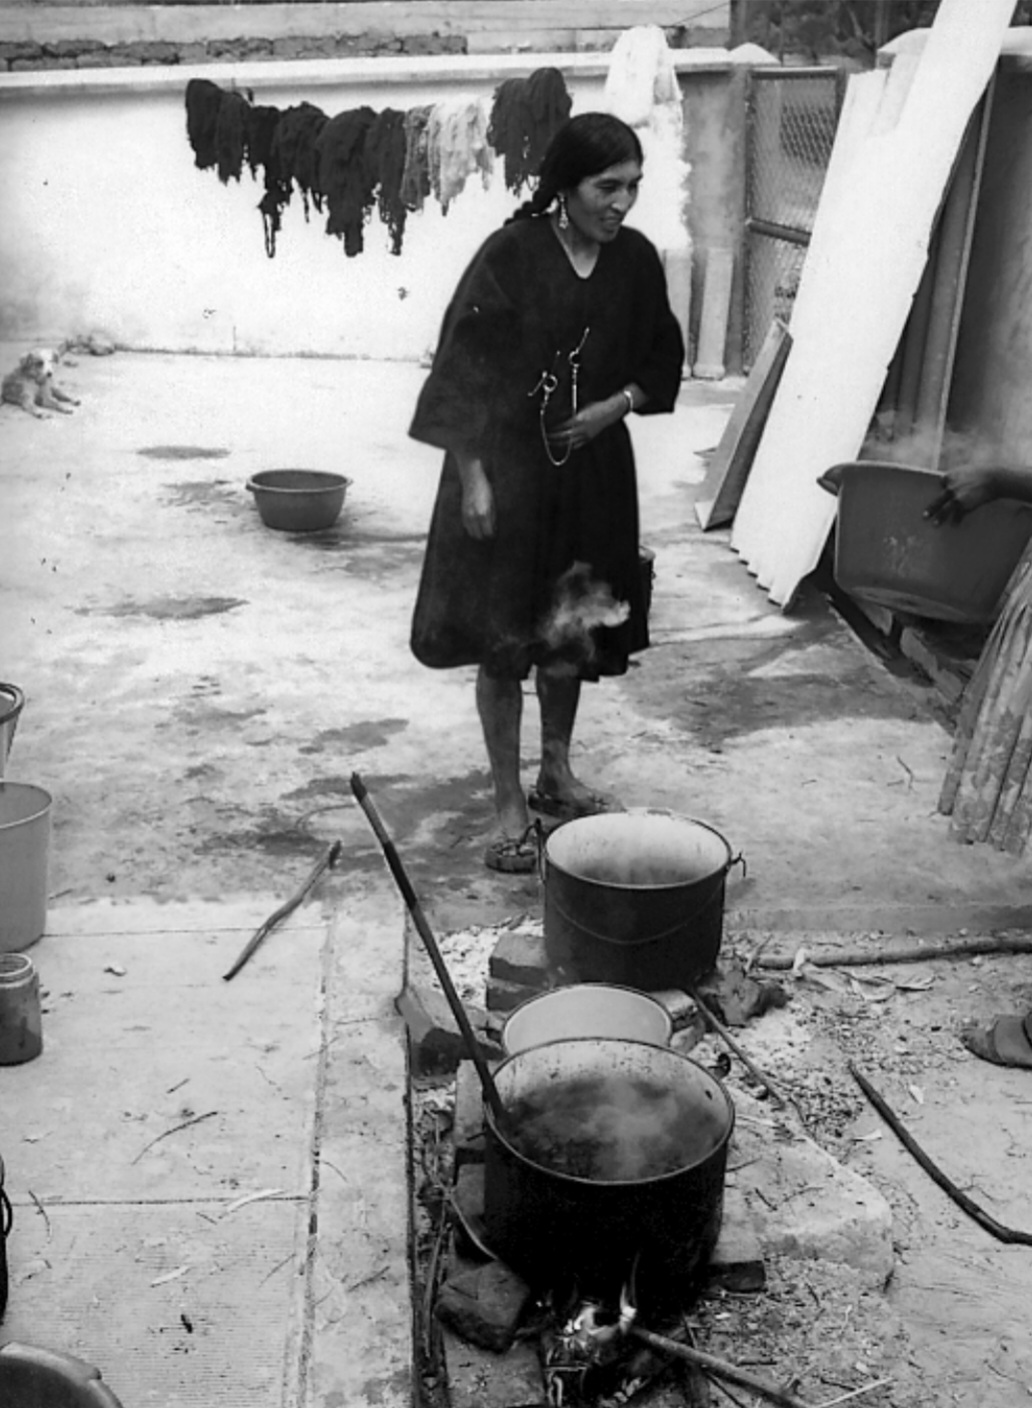
\includegraphics[width=0.6\textwidth]{figuras/cap.3/guaman_poma_acllaconas_fiando.png}
  \caption[\textit{Acllaconas} fiando, em Guaman Poma (1615)]{As \textit{acllaconas}, \enquote{mulheres escolhidas} ou \enquote{virgens do Sol}, em pleno trabalho de fiação. O desenho é a única imagem de que Urton dispõe de pessoas a fiar a matéria de que se faziam os \textit{khipu}, e as figuras retratadas são mulheres.\protect\footnote{A imagem não é registro direto da prática inca, e sim um desenho situado. Guaman Poma de Ayala, autor andino letrado, desenhou-a a pena e tinta por volta de 1615, entre as quase quatrocentas ilustrações de página inteira da \textit{Nueva corónica y buen gobierno}, manuscrito que escreveu e ilustrou pela própria mão como carta ao rei da Espanha. Como não havia, nos Andes, tradição pré-hispânica de imagens em tinta sobre papel, o desenho cruza convenções pictóricas europeias, a moldura, a composição, o texto alfabético junto à imagem, com a abstração geométrica dos têxteis e da cerâmica andinos \parencite{Adorno2000Writing}. A cena chega a Urton, e a mim, já traduzida por essa mão e por esse propósito, o que não a desqualifica como fonte, mas a inscreve, ela também, numa posição.}}
  \label{fig:acllaconas_fiando}
  \fonte{Guaman Poma de Ayala (1615, fol.~298 [273]), reproduzido em \textcite[fig.~5.3]{urton2003signs}. Fac-símile digital disponível em: \url{https://poma.kb.dk/permalink/2006/poma/298/es/image/}. Acesso em: 14 jun. 2026.}
\end{figure}

Há, porém, uma diferença que me interessa guardar, e que não desfaz a aproximação, antes a torce. Os números da computação eletrônica, e os da inteligência artificial, também contam histórias, mas o fazem ao contrário do \textit{khipu}. Onde o cordel inscreve a conta e o conto em um só gesto, à flor da matéria, o número eletrônico se faz signo cuja serventia é justamente comprimir a história, abstraí-la do fio, do corpo e do lugar de onde partiu, e fazê-la circular leve e combinável. O \textit{khipu} mostra a sua trama; o número a esconde. A história não desaparece, mas tem de ser desencavada, porque cada passo da cadeia ganha em forma, em combinabilidade e em mobilidade o que perde em localidade, em particularidade e em matéria \parencite{Latour2017Esperanca}. É esse soterramento, e não a ausência de narrativa, o que separa o cordel andino da grade de coeficientes a que chego no \texttt{Spira}. Pensar com essa outra figuração, a do cordel que conta e reconta, números e estórias, faz o trabalho, no sentido de Haraway, de não naturalizar a figuração herdada. A tabulação mecânica de Hollerith, à qual chego em seguida, é uma forma de contar entre outras possíveis, e o capítulo~\ref{capitulo4} reencontrará essa indistinção entre calcular e narrar no \texttt{Spira}, onde a voz de um paciente é ao mesmo tempo calculada em coeficientes e narrada como sintoma, como vírus e como enfermaria.

\begin{figure}[!htb]
  \centering
  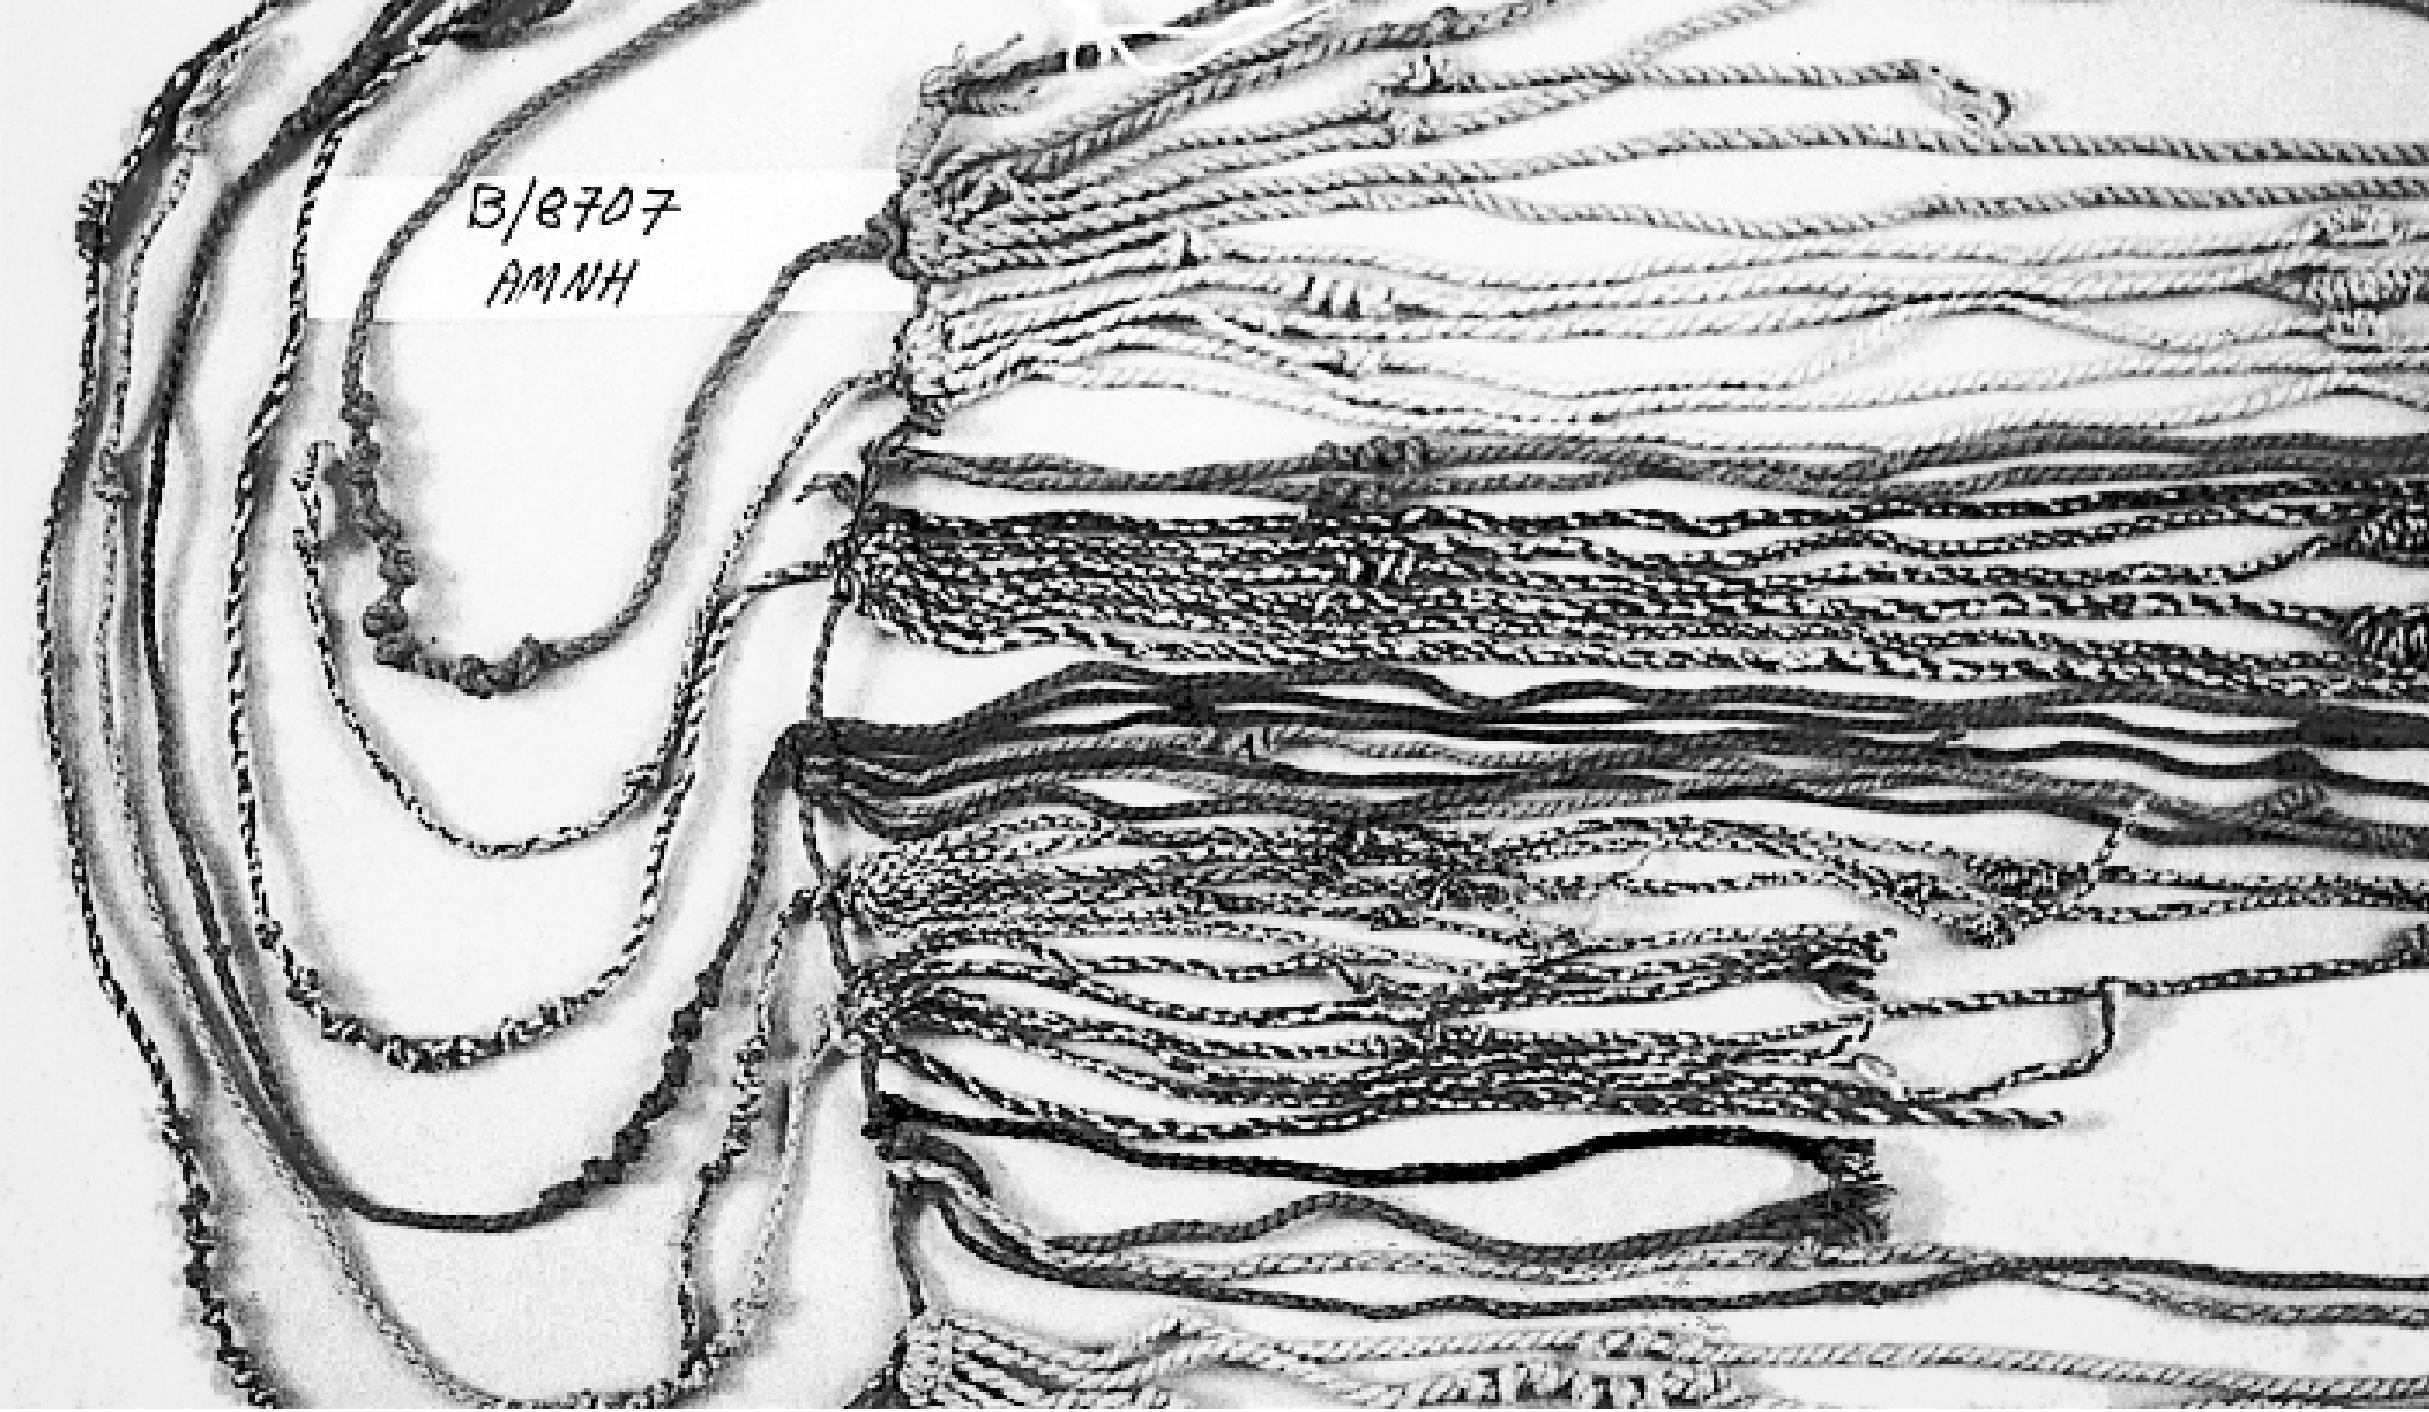
\includegraphics[width=0.6\textwidth]{figuras/cap.3/khipu_chancay_huando_amnh_b8707.png}
  \caption[\textit{khipu} da região de Chancay-Huando (AMNH B/8707)]{\textbf{\textit{khipu} da região de Chancay-Huando, costa central do Peru (AMNH B/8707).} O cordel principal, à esquerda, recolhe os cordéis pendentes em que a informação se inscreve pela cor, pela direção da fiação e da torção do fio, pelo sentido em que cada nó é atado e pela posição que ocupa. Urton lê esse aparato como exemplo de codificação binária, com cada traço abrindo uma escolha entre dois estados. Reproduzido de \textcite[p.~64]{urton2003signs}; acervo do \texttt{American Museum of Natural History}.}
  \label{fig:khipu_chancay_huando}
\end{figure}

Há uma escala nova em questão quando chego a Hollerith. O mesmo movimento de industrialização e urbanização que, nas sociedades modernas, fez crescer e adensar as populações fez também crescer a tarefa de contá-las, até que a contagem manual não desse mais conta: o censo estadunidense de 1880 levara cerca de oito anos para ser tabulado à mão, e o de 1890, diante de uma população ainda maior, ameaçava não ficar pronto antes do censo seguinte, e foi a esse impasse de escala que a tabulação por cartão perfurado de Hollerith respondeu \parencite{Austrian1982Hollerith}. Há aqui, portanto, uma relação de correspondência, em que contar uma população em escala industrial é parte do mesmo processo que produziu as populações a contar e os meios de o fazer. Com essas máquinas, observam Wiggins e Jones, tornou-se concebível registrar uma nação inteira num único arquivo manipulável de forma mecânica, e os grandes esforços de coleta fizeram do Estado, da população e da economia objetos de um novo tipo de conhecimento e de ação \parencite{Wiggins2023Data}.

Mas a máquina tabuladora automatiza em escala industrial o que outras sociedades, como a andina com os \textit{khipus}, já faziam de outra maneira: computar é uma prática antiga, plural e situada. A tabuladora e o \textit{khipu} são dois entre tantos objetos técnicos de contagem que precederam o computador eletrônico e o cercam, ao lado dos ossos entalhados com marcas do paleolítico africano, das fichas de argila (\emph{tokens}) com que a Mesopotâmia registrava bens antes mesmo da escrita, do ábaco em suas muitas formas, da Roma antiga ao \textit{suanpan} chinês e ao \textit{soroban} japonês, e da régua de cálculo dos engenheiros até há poucas décadas, cada um contando à sua maneira e com a sua matéria, sem que um seja ensaio de progresso do seguinte. Se ao cordel se atribui, entre outros usos, o registro de censos e tributos para um Estado, e à máquina de Hollerith o mesmo para outro, é porque contar uma população é sempre um modo de a tornar cognoscível por quem conta, à flor da matéria no \textit{khipu}, soterrado no cartão perfurado. D'Ignazio e Klein argumentam que decidir o que entra na contagem, e como se classifica o que foi contado, é ele próprio exercício de poder, e que esses sistemas se naturalizam como \enquote{o jeito que as coisas são} até que uma controvérsia os reabra; elas nomeiam ainda o paradoxo da exposição, a dupla amarra em que quem mais teria a ganhar ao ser contado é também quem mais se arrisca ao sê-lo \parencite{DIganzio2020Data}.

Essa relação entre contar, classificar e governar encontra ressonância desde Michel Foucault com o conceito de \textit{governamentalidade}, e é pensando com esse conceito, também, que sigo a trajetória da \texttt{IBM}.\footnote{Tomo a governamentalidade no sentido que Foucault assenta no curso \textit{Segurança, Território, População}: a arte de governar que toma a população por objeto e a economia política do saber, e que, em vez de proibir pela lei ou disciplinar corpo, conduz as condutas pela regulação de regularidades no nível do agregado, trabalhando com o provável e o aleatório, com taxas, médias e curvas de distribuição \parencite{Foucault2008Seguranca}. A biopolítica, que Foucault desenvolve nos cursos seguintes, é uma das tecnologias desse governo da população, a que incide sobre os processos biológicos da espécie, o nascer, o adoecer, o respirar e o morrer, tomados como objeto de cálculo e de gestão \parencite{Foucault2008Biopolitica, Foucault1999Defender}. Cito a distinção sem alongá-la, dado o quanto esses conceitos já foram discutidos nas ciências sociais, e guardo dela a ideia de que conhecer a população e governá-la são parte do mesmo processo, e que isto incide tanto sobre o agregado demográfico quanto sobre as vidas humanas e não humanas que o compõe.} A estatística, argumenta Foucault, é uma condição técnica da governamentalidade: a população só passa a ser governada dessa maneira depois que certos aspectos da vida, como a natalidade, a morbidade e a mortalidade, se fazem indicadores e, assim, categorias que podem ser computadas. O que guardo do conceito é que se trata de uma forma de poder que governa uma população desde o próprio ato de torná-la conhecida estatisticamente, e é isso que permeia a estatística setecentista, as máquinas tabuladoras de Hollerith e, a partir delas, a IA preditiva, que herda e radicaliza o cálculo de regularidades sobre populações. Vale notar que o estatístico Leo Breiman, ao mapear o seu próprio campo, separou essas formas de calcular não como dois métodos, mas como duas \enquote{culturas}, isto é, dois modos de crença sobre o que os dados são e sobre o que conta como conhecimento válido.\footnote{Em \enquote{Statistical Modeling: The Two Cultures}, Breiman opôs duas culturas no uso da modelagem estatística: uma que supõe os dados gerados por um modelo estocástico dado e busca explicá-los, e outra que trata o mecanismo gerador como desconhecido e usa modelos algorítmicos apenas para predizer \parencite{Breiman2001Cultures}. À primeira ele atribuía a quase totalidade dos estatísticos, e descrevia a adesão a ela em termos quase religiosos, em que o modelo, uma vez feito, se torna verdade; a segunda, minoritária à época e povoada por jovens da computação, é a que veio a prevalecer e da qual descende o que hoje se chama \emph{predictive modeling} (modelagem preditiva), \emph{predictive analytics} (análise preditiva) em uso comercial, assentada no \emph{machine learning} (aprendizado de máquina), em especial no aprendizado supervisionado, que aprende padrões a partir de exemplos rotulados para estimar desfechos em casos novos. O que ela busca é acertar o que ocorrerá, e contenta-se com correlações que funcionem, sem relação de causa estabelecida. Que um estatístico tenha nomeado a divisão como de culturas, e não de técnicas, é importante, pois a passagem ao cálculo preditivo é uma disputa situada dentro da própria tecnociência que são bases para a IA. Há ainda um grau seguinte, a \emph{prescriptive analytics} (análise prescritiva), em que a diferença para a preditiva é a de quem decide. A análise preditiva estima o que vai acontecer e entrega esse cálculo a uma pessoa, que decide o que fazer com ele; a prescritiva acrescenta à predição um aparato de regras e de otimização que já recomenda, e por vezes executa, a ação a tomar, de modo que a decisão antes reservada a quem recebia o cálculo passa a ser delegada ao próprio sistema. É nessa delegação que reconheço a passagem da predição ao controle de que trato adiante, é a computação, e não mais quem a recebe, que passa a decidir.} 

Essa leitura não é só de Breiman. Nos estudos de ciência e tecnologia, Johnson e Lenhard descrevem culturas de predição em que a matematização, a epistemologia, a tecnologia e a organização social do trabalho científico coevoluem, de modo que cada modo de predizer carrega consigo uma forma de fazer ciência e de organizá-la \parencite{JohnsonLenhard2024}. As duas fontes, de campos distintos, convergem em que predizer é uma prática situada, atravessada por crenças, técnicas e poder. Aprendi isso também de dentro, ao fazer os cursos de estatística e de aprendizado de máquina que descrevo no capítulo~\ref{capitulo1}. Logo na primeira aula, o professor abriu o curso afirmando que a probabilidade é um tipo de pensamento que se aprende, e não uma teoria, e que importa ter dela um conhecimento intuitivo, pois há \enquote{toda uma intuição por trás} dos métodos (figura~\ref{fig:caderno-rodrigues-aula1}).\footnote{Anotações do meu caderno de campo da primeira aula do curso \textit{Fundamentos de Probabilidade e Estatística para Ciência de Dados} (ICMC-USP, Prof.~Dr. Francisco~A. Rodrigues), em 28 de julho de 2025 \parencite{Rodrigues2024ProbEstat}. As frases entre aspas reproduzem o que registrei da fala do professor durante a aula.} Naquela aula, ele distinguiu a inferência da predição por dois verbos, inferir é encontrar, predizer é adivinhar, e apresentou a estatística bayesiana como uma \enquote{atualização da crença}, em que uma probabilidade inicial, o \emph{priori}, se revê diante de novos dados. Em uma aula seguinte, ao introduzir a simulação computacional, definiu o computador como o laboratório onde se aprendem esses conceitos. Tomadas em conjunto, essas formulações de campo exemplificam a virada de que trato aqui: o cálculo probabilístico é ensinado como um modo de pensar, atravessado por intuição e por crença, e não como teoria neutra; a sua finalidade desloca-se do encontrar ao adivinhar, da inferência que busca a estrutura à predição que estima o que vem; e o seu lugar de exercício passa a ser o computador, que simula, calcula e prediz. É nesse deslocamento, da estatística para a computação, que a cultura preditiva se assenta. Essa história, a que liga a estatística e classifica ao cálculo preditivo computacional, já foi investigada por Wiggins e Jones ao argumentarem que os dados são produzidos, e que censos e levantamentos constituem a população como objeto de ação governamental, chegando por essa via a Foucault e à historiografia da quantificação dos povos \parencite{Wiggins2023Data}. Retomo essa história de um jeito diferente, por meio da etnografia do \texttt{C4AI} e de documentos, em que os relatórios anuais, o Acordo de Cooperação e as comunicações institucionais do \texttt{C4AI} e da \texttt{IBM} me deixam seguir. A trajetória de mais de um século que sigo neste capítulo é essa história lida de uma posição situada, a de quem acompanhou um arranjo entre universidade pública e corporação e o viu encerrar-se.

A principal diferença ocorre, sobretudo, na escala e na direção que a IA atual toma. Onde o censo contava o que acontecia ou o que já havia acontecido, os sistemas de IA de hoje calculam o que ainda não aconteceu e fornecem material para se pensar e agir sobre o conteúdo da predição; por exemplo, ao estimar a probabilidade, isto é a chance de um determinado evento ocorrer, de uma região concentrar crimes e para lá dirigir o policiamento, ao atribuir a cada pessoa um escore de crédito que decide quem obtém empréstimo, ou ao ordenar, em uma fila de atendimento em saúde ou de benefício social, quem é triado primeiro. Lidar com a incerteza do futuro para decidir sobre o presente é mais antigo que a IA. A própria probabilidade, condição da governamentalidade de que trato, já era uma forma de fazê-lo, calcular regularidades, estimar o provável, calcular os riscos, saber quais são as chances. O que a IA preditiva acrescenta é uma pretensão nova, a de controlar o futuro, e não só de calculá-lo, mas também para agir desde já sobre o que ainda não aconteceu para que aconteça, ou deixe de acontecer, conforme o planejado. O policiamento que se dirige a uma região antes do crime, o crédito que se nega antes da inadimplência, a triagem que se decide antes do agravo; em cada caso, a predição intervém no porvir mais do que o descreve. Vale, de passagem, um paralelo que tomo com parcimônia, com o oráculo de veneno que Evans-Pritchard descreveu entre os Azande que era também um modo de decidir diante do incerto, e era sobre o seu veredito que se julgavam disputas e se lançavam sentenças \parencite{EvansPritchard2005Bruxaria}. A confiança no oráculo vinha da imprevisibilidade da reação da ave, daquilo que escapava ao cálculo humano; a confiança na IA vem do oposto, de ela pôr a incerteza em números, ao dizer que algo tem tantos por cento de chance de acontecer ou não acontecer, e é esse grau de certeza calculado a partir de exemplos passados que a faz ter tida confiável e governável.

\begin{figure}[H]
  \centering
  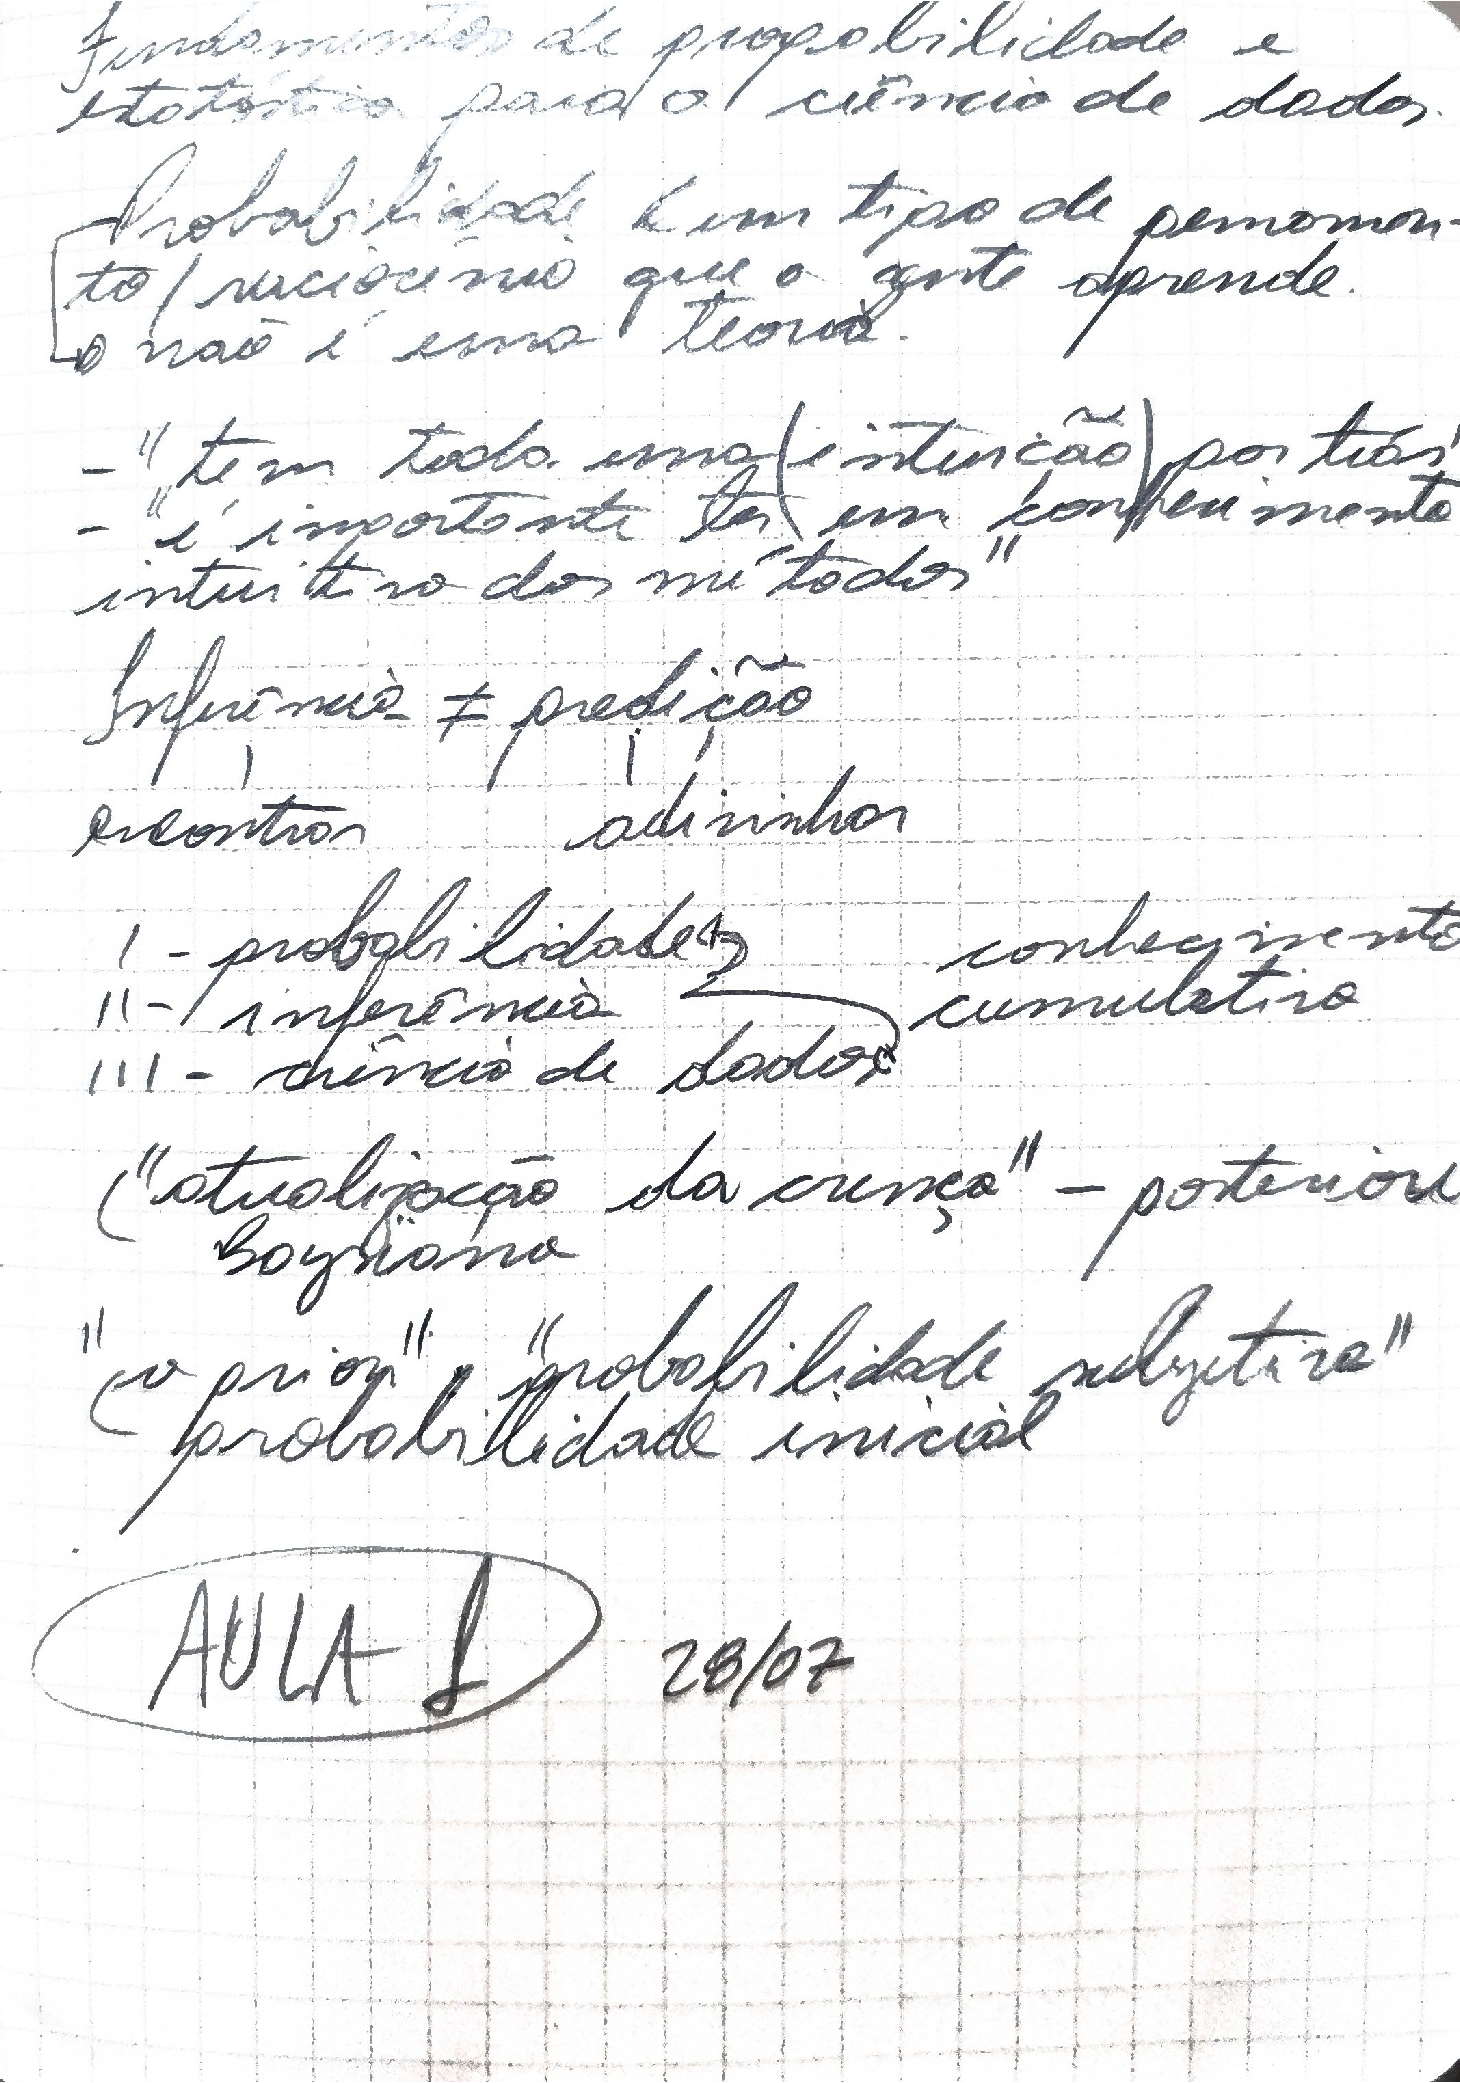
\includegraphics[width=0.85\textwidth]{figuras/cap.3/caderno_rodrigues_aula1.pdf}
  \caption[Caderno de campo: primeira aula do curso de probabilidade e estatística (28/07/2025)]{Página do meu caderno de campo referente à primeira aula do curso \textit{Fundamentos de Probabilidade e Estatística para Ciência de Dados} (ICMC-USP, Prof.~Dr. Francisco~A. Rodrigues), em 28 de julho de 2025. As anotações registram que a probabilidade é \enquote{um tipo de pensamento/raciocínio que a gente aprende} e que \enquote{não é uma teoria}, que \enquote{tem toda uma intuição por trás} e que \enquote{é importante ter um conhecimento intuitivo dos métodos}; a distinção \enquote{inferência $\neq$ predição}, glosada pelos verbos \enquote{encontrar} e \enquote{adivinhar}; o encadeamento \enquote{probabilidade $+$ inferência $+$ ciência de dados} como \enquote{conhecimento cumulativo}; e a estatística bayesiana como \enquote{atualização da crença}.}
\label{fig:caderno-rodrigues-aula1}
\end{figure}

Desta maneira, a estatística do censo descrevia a população que contava; a IA preditiva vai além e antecipa o que dela se deixa prever, os comportamentos, os riscos, tudo o que se possa estimar como provável a partir do que já foi coletado de exemplos ocorridos no passado. A pandemia de Covid-19 mostrou como isso vem ocorrendo. Os doentes viravam curvas de infectados, taxas de transmissão, projeções de óbitos e de ocupação de leitos, e era sobre esses números que se passou a decidir as medidas de saúde pública. Cada pessoa adoecida entrava no cálculo como ponto de uma curva, do mesmo modo como, no cartão de Hollerith, cada pessoa entrara como categoria perfurada; em ambos, a vida singular se faz dado agregado, e é nessa forma que se torna governável. Esse modo de tornar a vida computável segue em funcionamento e se intensificou como nunca antes. Digitalizar a saúde converte o prontuário em arquivo legível por máquina, datificá-la vai além, e faz do sintoma físico do corpo, do exame e do diagnóstico do paciente pontos de dado sobre os quais se calcula e se decide, como faço no caso do \texttt{Spira}.\footnote{Configurações como essa vêm sendo nomeadas como datificação da vida. O termo \emph{datafication} foi cunhado por \textcite{MayerSchonberger2013Big} para o gesto de pôr um fenômeno em forma quantificada de modo que possa ser tabulado e analisado, e foi deslocado, na crítica que se lhe seguiu, para nomear a conversão da própria vida social em dado e a extração de valor que essa conversão alimenta \parencite{vanDijck2014Datafication, CouldryMejias2019Costs}. O Programa SUS Digital, instituído no Brasil em 2024 e com adesão de todos os 5.570 municípios, dos 26 estados e do Distrito Federal, é um exemplo dessa intensificação. Descreve-se como um conjunto de iniciativas que modernizam o Sistema Único de Saúde por soluções digitais e tem entre suas metas o prontuário eletrônico, o acesso do cidadão aos próprios dados no aplicativo Meu SUS Digital e painéis de monitoramento e relatórios de desempenho que o gestor mobiliza para a tomada de decisão. Disponível em: \url{https://www.gov.br/saude/pt-br/composicao/seidigi/sus-digital}. Acesso em: 16 jun. 2026. Datificar a saúde pode ter efeitos sobre a vida das pessoas, ao antecipar um agravo, ao distribuir melhor um leito, ao devolver ao paciente o acesso ao próprio histórico, etc. O que decide a qualidade desses efeitos é o arranjo que o sustenta, de quem é a infraestrutura que guarda os dados, quem os gere, com quem são compartilhados e a serviço de que fim, questões que retomo no capítulo~\ref{capitulo4} ao seguir o \texttt{Spira} até as condições materiais e institucionais de que depende.} Computar uma população e geri-la passam a ser a mesma coisa, e foi na tecnociência da tabulação que isso deu seus primeiros sinais em escala industrial, quando o censo de 1890 converteu a vida das pessoas em categorias perfuradas no cartão (sexo, raça, idade, nacionalidade, estado civil, profissão, residência). Considero, porém, outras populações. As redes da IA, e as que aqui descrevo, abrangem também não humanos, animais, plantas, territórios, e alcançam, no limite, aquilo que sequer se tem por vivo, os recursos minerais, o clima, um vírus como também sigo no capítulo~\ref{capitulo4}. No \texttt{Spira}, esse converter-se da vida em dado toma a forma de uma cadeia de inscrição: o fôlego de uma pessoa torna-se sinal de áudio, espectrograma e, por fim, coeficiente processável por uma rede neural, no movimento que sigo no capítulo~\ref{capitulo4}. E esse mesmo cálculo, que parece imaterial, repousa sobre um fundo material: há, do outro lado, todo um não vivo arrancado da terra para que a conversão se faça. O mineral, o inerte que o poder extrai e converte em valor, é também a base material da IA,\footnote{A fronteira entre o que conta como vida e o que conta como inerte é o que Elizabeth Povinelli chama de partição entre a Vida e a Não Vida, sobre a qual se exerce o \textit{geontopoder}, modo de governança do liberalismo tardio que separa o domínio do orgânico do domínio do geológico, da rocha e do mineral \parencite{Povinelli2023Geontologias}. É desse \textit{geos}, o polo da Não Vida que o poder extrai, que volto a tratar adiante.} e é o que os estudos críticos rastreiam quando seguem as cadeias globais de extração material, laboral e epistêmica que sustentam esses sistemas, do lítio e do cobalto das minas ao trabalho de quem rotula dados, em especial Crawford e Joler \parencite{Crawford_Joler_CalculatingEmpires_2023, Crawford2018Anatomy} e Pasquinelli \parencite{pasquinelli2020nooscope, Pasquinelli_EyeMaster_2023}.

Há um movimento que me detém neste percurso, e que as figuras do \textit{geos} e do Terrestre me ajudam a pensar. O minério que sustenta a inteligência artificial levou eras geológicas para se depositar na crosta, e quanto mais essa tecnologia se anuncia como futuro, como salto adiante rumo a um mundo cada vez mais tecnológico, mais ela desce ao fundo do tempo da Terra. O circuito que promete o porvir é feito de lítio, de cobalto, de silício, de terras raras, e o vetor que parecia apontar para a frente aponta, ao mesmo tempo, para baixo, para o mineral de que a tecnologia nunca se desprende. Latour dá nome a essa torção quando recusa a flecha que ia do Local atrasado ao Global futuro e a substitui pelo movimento do Moderno ao Terrestre, um descer à terra, algumas dezenas de quilômetros, a Zona Crítica, entre a atmosfera e a rocha, em que a vida e a técnica de fato se sustentam \parencite{Latour2020Onde}. Leio nisso, mais do que um regresso ao passado que apenas reinscreveria a mesma flecha ao contrário, a descoberta de que o futuro tecnológico nunca esteve à frente, e sim embaixo, na matéria de que sempre dependeu.

Antes de seguir essa torção, demoro-me no que a conta dos minérios e dos dados quase sempre deixa de fora: as inúmeras comunidades de seres vivos, humanas e não humanas, que habitam os territórios de onde se extrai a matéria da inteligência artificial, e cujos mundos a mineração desfaz no mesmo gesto com que arranca o minério. É a mesma torção que o \textit{khipu} fez ver no início deste capítulo, quando desfez a linha reta que iria da máquina antiga à inteligência artificial, assim como, computar não foi a invenção de uma máquina por vir, mas permeia práticas antigas, plurais e situadas, o futuro da inteligência artificial parece correr à dependência cada vez mais profunda do \textit{geos}, do mais antigo e mais inerte dos não humanos. E aqui as duas figuras que evoco entram em tensão: o \textit{geos} de Povinelli é a Não Vida, o inerte que o poder extrai e converte, ao passo que o Terrestre de Latour é um \enquote{geo} que reage, que deixou de ser o plano de fundo da ação humana para participar dela, voltando-se contra quem o explora \parencite{Latour2020Gaia}. A inteligência artificial trata o \textit{geos} como matéria, minério a extrair e dado a processar, mas é esse mesmo \textit{geos} que reage, no esgotamento das jazidas e na reação do sistema terrestre, e se recusa a permanecer inerte. Retomo, assim, o fio que assentei no capítulo~\ref{capitulo1}: se ali a rede já não distinguia o humano do não humano, aqui ela não distingue sequer o vivo do inerte, e o mineral, o mais mudo dos actantes, mostra-se capaz de agir. É esse adensamento do \textit{geos} na tecnologia, e a sua recusa em ser mero recurso, o que sigo ao descer com os atores até à Terra de que empresas como a \texttt{IBM} e centros de pesquisa como o \texttt{C4AI} extraem e constroem suas tecnociências. 

Se até a Terra (rea)age, como sustentei há pouco, é porque a rede que sigo não conhece hierarquia entre os seus actantes, e isso exige precisar o que entendo por rede e por agência, a noção que me autoriza a seguir, em um mesmo plano, Fábio, Cláudio, a \texttt{IBM} e a máquina tabuladora. Compreendo a rede, neste capítulo, como um processo de articulação entre atores --- ou actantes, quando quero enfatizar (e não diferenciar), a agência não humana ---\footnote{Uso \enquote{actante} para realçar a agência não humana, no sentido que desenvolvi no capítulo~\ref{capitulo1}, e, como Latour, alterno actante e ator conforme o tipo de agência que quero pôr em relevo. A própria expressão ator-rede funciona como oxímoro, articulação de termos opostos que produz um sentido novo \parencite{latour1996clarifications}.} humanos e não humanos, cuja dinâmica depende de relações materiais, discursivas, simbólicas e institucionais. Interessa-me, sobretudo, o modo como as agências --- e entendo por agência qualquer entidade que age ou à qual uma ação é atribuída, sem supor motivações humanas --- se distribuem pela rede e como se transformam, ao longo do tempo, em distintos regimes sociotécnicos. A rede é, então, a associação entre actantes heterogêneos, individuais ou coletivos, que se definem em boa parte ao longo das próprias cadeias de associação; aquilo que se move e aquilo que é movido não tem forma nem atributos estáveis, e cada ator ganha contorno a partir das relações que estabelece com os outros \parencite{latour1996clarifications}. É esse o sentido em que sigo com Latour e Callon ao longo deste capítulo, e é também o que me permite tratar a translação como a descrição do que sobrevém aos atores e aos objetos quando se associam.

\section{Seguindo Fábio e Cláudio: observação, entrevistas e documentos}
\label{sec:seguindo_atores}

Quando iniciei a pesquisa, o centro estava em consolidação e buscava pesquisadores, financiadores e infraestrutura, que eu denomino por \textbf{aliados}. Tomo \enquote{aliados} e \enquote{alianças} no sentido latouriano de atores, humanos e não humanos, vivos e não vivos, recrutados para sustentar uma controvérsia e estabilizar fatos e artefatos das tecnociências. É vocabulário que pertence à figuração militar-industrial cuja densidade e cujos efeitos analiso no capítulo~\ref{capitulo2}, e o uso aqui com essa consciência. Latour descreveu a ciência como os próprios cientistas a apresentavam e a praticavam, e o vocabulário militar não é, nele, escolha estilística do analista, mas a forma que essa prática assumia em ação. Fábio e Cláudio faziam essa tecnociência. Buscar pesquisadores, financiadores e infraestrutura, sustentar a controvérsia que mantinha o centro de pé, vencer a disputa por recursos, era recrutar aliados no sentido exato em que Latour descreve o gesto, e descrevê-lo assim é fiel ao que eu via em campo. A figuração têxtil de Haraway, que sustento no capítulo~\ref{capitulo2}, faz outra coisa, porque propõe um outro tipo de tecnociência, e eu a mobilizo como figuração de pensamento e como o lugar de onde escrevo esta tese, e não como descrição do que Fábio e Cláudio faziam. Quando descrevo o trabalho deles, descrevo como Latour, porque era assim que eles trabalhavam; quando me posiciono sobre que tecnociência quero fazer, e como quero descrevê-la, é com Haraway que penso. Manter essa distinção visível é o que me permite usar o vocabulário militar aqui no capítulo~\ref{capitulo3} sem o naturalizar, isto é, como figuração que descreve uma prática situada, e não como a única forma de dar a ver o que o centro fazia.\footnote{Eu também me tornei uma \enquote{aliada} e, além de realizar esta pesquisa sobre eles, passei a fazer parte do grupo de humanidades do \texttt{C4AI}, o Observatório de IA: impactos e regulação (\texttt{OBIA@C4AI}).} Essa presença em toda parte foi ainda amplificada pelo isolamento da pandemia de Covid-19 (2020-2023), que afastou os encontros presenciais e empurrou a vida do centro para os espaços públicos controlados e digitais em que eu os encontrava, esses mesmos espaços que configuraram o que seria um laboratório de inteligência artificial para esta tese, conforme discuto nos capítulos~\ref{capitulo1} e~\ref{capitulo4}.\footnote{Apresentei a origem institucional do \texttt{C4AI}, sua fundação em outubro de 2020 em plena pandemia, o arranjo \texttt{USP}-\texttt{FAPESP}-\texttt{IBM} no âmbito dos Centros de Pesquisa em Engenharia da \texttt{FAPESP} e a configuração do centro como laboratório distribuído, no capítulo~\ref{capitulo1}. Retenho aqui o que importa ao argumento deste capítulo. O \texttt{C4AI} conta ainda com três instituições associadas, \texttt{ITA}, PUC-SP e \texttt{FEI}, e integrava a \texttt{IBM} AI Horizons Network (AIHN), rede global de centros de pesquisa universitários que a \texttt{IBM} estabeleceu em 2016 para \enquote{acelerar pesquisa e aplicação de IA} através de colaborações com \enquote{universidades líderes}. Essa formulação pede análise, ao posicionar a \texttt{IBM} como articuladora central de uma rede global em que as universidades, ainda que descritas como \enquote{líderes}, atuam dentro de um ecossistema estruturado por prioridades e infraestruturas corporativas. Para informações institucionais do \texttt{C4AI}, ver: \url{https://c4ai.inova.usp.br/about.html}. Acesso em: 30 nov. 2025.} Foi assim que Fábio e Cláudio passaram a comparecer falando em nome do centro como porta-vozes,\footnote{Retomo \enquote{porta-voz} no sentido que assentei no capítulo~\ref{capitulo1}, o de quem fala em nome de entidades, humanas ou não, que dependem de alguém que articule suas posições. Fábio e Cláudio compareciam como porta-vozes do \texttt{C4AI} ao apresentá-lo e representá-lo nos espaços que acompanhei.} atraindo para si as atenções, inclusive a minha. Era comum que apresentassem o centro e suas pesquisas, e a \texttt{IBM} surgia com frequência nessas conversas. \enquote{Quando o C4AI começou havia uma certa dificuldade de saber se a gente ia conseguir agregar tanta gente e como é que a gente ia fazer isso}, contou-me Fábio em entrevista. Foi a participação da \texttt{IBM} que trouxe foco: em \enquote{vários encontros no começo}, definiram \enquote{que não ia fazer muitos projetos para não pulverizar o dinheiro}, e o centro tornou-se \enquote{um centro que, em volta de alguns projetos, que exigem conhecimento de várias fontes, de várias áreas, você tem todo um grupo de gente interessada em IA}.

Ao longo do tempo, porém, essa concentração teve seus efeitos. Quando a \texttt{IBM} reorientou seus interesses nas frentes de saúde e de agronegócio, os projetos correspondentes perderam o financiamento direto do centro, e o quanto a agenda de pesquisa se atava às decisões estratégicas corporativas, que o cotidiano mantinha implícito, tornou-se mais evidente. O \texttt{C4AI}, por sua vez, não parou onde a frente corporativa parou. No mesmo período em que a \texttt{IBM} deixava o setor de saúde, os pesquisadores do centro montaram um centro dedicado ao tema, o Centro de Inteligência Artificial em Gestão em Saúde, aprovado pela \texttt{FAPESP} em 2024, e, enquanto a frente do agronegócio se reorientava, desenvolveram o MClimate, novo desafio de pesquisa voltado à previsão climática por modelagem física. Em ambos os casos, uma frente que perdia o aporte corporativo reaparecia sob outro arranjo de financiamento e outro recorte de pesquisa, por iniciativa dos próprios pesquisadores, e desse percurso resultaram publicações científicas, \textit{datasets} abertos e ferramentas disponibilizadas à comunidade. Deslocamentos como esses são descritos neste capítulo, e não a intenção que os teria guiado nem uma ordem em que a corporação se moveria primeiro e o centro reagiria depois: não tenho como dizer, a partir do que pude seguir, se reancorar uma frente em nova fonte de fomento foi gesto de autonomia diante da \texttt{IBM} ou recomposição da mesma atadura sob outra forma, e as negociações em que isso se decidiu correram por canais que não acompanhei. Descrevo, então, uma rede em que cada ator, corporação, universidade, agência de fomento e pesquisadores, faz associações e desloca o curso das associações, e deixo em aberto o que cada deslocamento significou.

Caminhei conforme fosse preciso, acompanhando as associações onde quer que elas me levassem, e elas pareciam levar-me a Fábio e Cláudio, bem como ao que faziam e diziam. Eles, porém, foram dois entre os atores que acompanhei (como demonstro no capítulo~\ref{capitulo4}, ao apresentar a rede construída por Marcelo). Também observei outros atores e eventos, muitos dos quais ficaram fora da versão final desta tese, mas que estão presentes na perspectiva analítica desta pesquisa e no olhar etnográfico que a permeia. As fronteiras que limitam a extensão da rede a traçar (teórica ou metodologicamente) não estão dadas, e ainda assim preciso começar e parar em algum ponto, ao menos para os fins e objetivos práticos da pesquisa. A ausência de determinados atores é tão consequente analiticamente quanto a sua presença, seja essa ausência intencional ou não. Foram os movimentos desses atores que me levaram a escrever este capítulo, seguindo o caminho que eles me indicavam e que eu queria seguir.

Algoritmos e modelos de linguagem apareceram ao longo dessa caminhada, emergiram na entrevista com Marcelo, em narrativas retrospectivas sobre o desenvolvimento do \texttt{Spira}, e nos artigos científicos que analisei (conforme discuto no capítulo~\ref{capitulo4}). O que me escapou foi o fazer IA em ato, o movimento de construção dos conjuntos de dados e dos modelos propriamente ditos diretamente pelas mãos dos cientistas e engenheiros. Encaro essa inacessibilidade como um limite desta etnografia, em lugar de saldá-la com uma explicação que eu não tenho como sustentar. O que pude seguir foram os relatos sobre esse fazer, e não o fazer no instante em que se dava --- e não seria isso uma maneira de também fazer? ---, e as razões desse limite excedem o que o meu material permite isolar; a pandemia, o modelo de laboratório distribuído e as dinâmicas particulares do \texttt{C4AI} compõem-se, no meu caso, com o que pode ser uma reserva mais ampla do campo diante da observação externa, sem que eu disponha de meios para separar o que pertence a cada um. Deixo a questão nesse ponto, como parte do que a posição de onde descrevo alcança e do que lhe escapa. Esse tipo de limitação, com o tempo, passou a constituir um dos argumentos desta pesquisa, pois Latour sustenta que a distinção entre o \enquote{interior} e o \enquote{exterior} de uma ciência é ela mesma efeito do trabalho científico. O que aparece como interior e o que aparece como exterior são dois lados de um mesmo divisor, erguido pela própria prática, e retomo esse argumento na Lição 1 do capítulo~\ref{capitulo1}, sobre acompanhar a pesquisa em IA enquanto ciência em construção. Lida por essa chave, a opacidade do núcleo técnico deixa de ser a parede em que minha observação esbarrou e passa a ser um efeito do corte que fiz, no sentido de \textcite{strathern2011cortando}.

Seguir Fábio e Cláudio significou estar onde eles estavam, e onde eles estavam era a rede pela qual o \texttt{C4AI} parecia funcionar naquele momento, sem paredes que a fechassem em um \enquote{laboratório} delimitado fisicamente, como discuto no capítulo~\ref{capitulo4} ao seguir a rede que Marcelo construiu.\footnote{Mantive diálogos com pesquisadores vinculados ao \texttt{C4AI} ao longo do trabalho de campo. Essas conversas, sem roteiro estruturado e sem o formato de entrevista formal, foram fonte de dinâmicas cotidianas, tensões não verbalizadas em contextos públicos e percepções sobre o arranjo que por vezes diferiam das narrativas institucionais. A pedido dos interlocutores, não as identifico nominalmente. A escolha responde a uma consideração ética, a de proteger pessoas em posição de menor poder institucional, que poderiam sofrer consequências por declarações críticas, e ao reconhecimento de que o caráter aberto dessas trocas dependia, em parte, da garantia de anonimato. Quando informações dessas conversas informam a análise, apresento-as de modo a preservar o anonimato sem comprometer a integridade interpretativa.} Essa posição tinha o seu preço. O \texttt{C4AI}, distribuído por quatro campi, dezenas de grupos, centenas de pessoas, só comparece como uma coisa só quando alguém o enuncia, e Fábio e Cláudio eram esse alguém. Ao dizerem o que o centro era e o que faziam os seus pesquisadores, não relatavam uma voz que o \texttt{C4AI} já tivesse; davam-lhe uma, e a que lhe davam recortava, entre tudo o que o centro era, a face que cabia no que diziam. Era essa face que eu acessava ao segui-los, nos eventos onde os encontrei. O cotidiano de quem desenvolvia os modelos, coletava os dados, escrevia o código e treinava os algoritmos corria em uma outra camada da rede. Seguir os porta-vozes me pôs diante das estratégias de legitimação, das tensões entre agendas corporativas e acadêmicas, das negociações que sustentam os arranjos de inovação, e deixou fora do meu alcance, as práticas laboratoriais distribuídas, as rotinas dos bolsistas, as decisões técnicas do desenvolvimento dos sistemas. A rede que Fábio e Cláudio teciam era uma parte do \texttt{C4AI}, e o centro permanecia maior do que ela. Sigo certos atores e, ao segui-los, deixo de seguir outros; é dessa parcialidade que esta etnografia se faz, e é ela que a tensiona.

O que descrevo, portanto, é o \texttt{C4AI} a partir de seus porta-vozes e das redes que eles construíam, e foi por aí que cheguei a certas relações que organizam os arranjos público-privados em inteligência artificial. Seguindo Latour, fazer ciência é manipular instrumentos, coletar dados e construir modelos no interior de um laboratório, e é também, e talvez sobretudo, alistar aliados, mobilizar recursos, negociar financiamentos, traduzir interesses, estabilizar redes que permitam aos fatos e artefatos circularem e se sustentarem. Em \textit{Ciência em Ação}, Latour acompanha um \enquote{chefe} de laboratório que passa semanas viajando entre ministérios, indústrias farmacêuticas e universidades, enquanto sua colaboradora permanece na bancada. \enquote{Quem está realmente fazendo pesquisa?}, pergunta Latour. \enquote{Onde é que a pesquisa está de fato sendo feita?} A resposta é que ambos fazem ciência: ela \enquote{é capaz de se dedicar inteiramente ao trabalho de laboratório \textit{porque} o chefe está sempre fora, trazendo para dentro recursos e subsídios novos}.\footnote{\textcite[p.~257]{Latour2011CienciaEmAcao}. Latour conclui: \enquote{a tecnociência tem um lado de dentro porque tem um lado de fora. [\ldots] quanto maior, mais sólida, mais pura a ciência é lá dentro, maior a distância que outros cientistas precisam percorrer lá fora} (p.~258). Seguir os porta-vozes do \texttt{C4AI} por seminários, eventos empresariais e negociações institucionais documentou, portanto, as condições que tornam possível esse fazer.} Fábio negociando com a \texttt{FAPESP}, Cláudio explicando à \texttt{IBM} como o centro pode atender às necessidades do setor, pesquisadores disputando acesso a GPUs, bolsistas publicando em conferências internacionais para legitimar o trabalho do centro: tudo isso é fazer IA. A distinção entre o \enquote{científico} e o \enquote{institucional}, entre o \enquote{técnico} e o \enquote{político}, é ela mesma um efeito das redes que deram certo, e só na aparência precede esse efeito. É uma etnografia do fazer IA nessa dimensão que ofereço, a que mostra as condições de possibilidade para que algoritmos existam, modelos sejam treinados, sistemas sejam desenvolvidos e pesquisas se sustentem no tempo.

Nas notas de campo registrei o que era dito e, com igual atenção, \textit{como} era dito, \textit{onde} era dito e \textit{para quem} era dito. Fábio e Cláudio apresentavam o \texttt{C4AI} de um modo nos contextos acadêmicos, com ênfase em metodologia, rigor científico e contribuições teóricas, e de outro nos contextos empresariais, com ênfase em aplicabilidade, parcerias estratégicas e geração de valor, e essa diferença mostra como a tecnociência circula por registros heterogêneos e se constitui nessa circulação, no transitar entre a universidade e o mercado. É o que Latour documenta no \enquote{chefe} de laboratório, que em um mesmo dia apresenta a pandorina ao ministro da Saúde enfatizando aplicações clínicas, aos colegas da Academia enfatizando rigor metodológico, aos jornalistas enfatizando revolução científica.\footnote{Cf. \textcite[p.~252--255]{Latour2011CienciaEmAcao}. O \enquote{diário} fictício que Latour constrói para acompanhar o chefe de laboratório documenta essa capacidade de circular entre registros heterogêneos: ministérios, indústrias, universidades, hospitais, matadouros.} Essa atenção ao modo do dizer só foi possível a partir de um lugar determinado. Eu estava na audiência daqueles eventos porque o vínculo com o OBIA, o grupo de humanidades do \texttt{C4AI}, me punha ali, e foi esse mesmo vínculo que me deu as discussões institucionais e as conversas informais a que de outro modo eu não chegaria. Anotava-as no caderno de campo que mantinha no aplicativo de notas do celular, e ao lado do que se dizia eu registrava a circunstância da minha presença: de onde eu escutava, como tinha chegado àquela sala, o que a minha entrada pelo OBIA me abria e o que, por ela, me ficava vedado. Ao integrar o OBIA, tornei-me parte da rede que investigava, e essa posição é ela mesma um dos cortes que torna presentes certas relações e deixa outras na sombra. Não há ponto de vista exterior de onde uma rede sociotécnica se deixe contemplar com objetividade, porque quem observa é parte das associações que descreve, e foi de dentro dessa condição que escrevi. O que me coube, então, foi anotar a circunstância da minha presença junto com o que ela me deixava ver, em vez de apagá-la para simular uma vista de lugar nenhum.\footnote{Como argumenta Latour, \enquote{seguir cientistas e engenheiros de verdade} exige \enquote{mais sutileza agora que nosso guia vai vestir muitas máscaras misturadas e seguir por caminhos vários simultaneamente} \parencite[p.~241]{Latour2011CienciaEmAcao}. O rigor está em explicitar a própria posição e os seus efeitos sobre o que dali se alcança e o que dali escapa, em vez de fingir uma neutralidade inexistente.}

Foi sobre esses anos de observação que as entrevistas se assentaram. Conversei com Fábio Cozman em 4 de setembro de 2025 e com Cláudio Pinhanez em 2 de outubro de 2025, cerca de sessenta minutos cada, depois de mais de três anos acompanhando o arranjo, o que me permitiu formular perguntas informadas pelas tensões que a observação havia me deixado entrever de forma fragmentária.\footnote{Ambas as entrevistas foram realizadas em português via Google Meet, transcritas integralmente e analisadas em língua original.} O modo direto com que os dois descreveram o arranjo, Cláudio explicitando a lógica de arbitragem geopolítica ao dizer que \enquote{o estudante é barato demais}, Fábio reconhecendo que projetos perderam financiamento quando a \texttt{IBM} vendeu divisões comerciais, devo em parte à confiança construída ao longo de anos, e em parte ao momento das conversas, realizadas quando o arranjo ainda vigorava no papel, mas já sob tensões que anunciavam seu fim. Foi numa conversa informal com pesquisadores de outros grupos do \texttt{C4AI}, aliás, que soube de algo ainda não público: quando entrevistei Fábio e Cláudio, a \texttt{IBM} já havia comunicado ao centro, em agosto de 2025, que não renovaria o cofinanciamento por mais cinco anos, como se esperava. A notícia só se tornaria pública em novembro. Eu fazia, portanto, as entrevistas com dois porta-vozes que já sabiam do fim, em um intervalo em que o arranjo se mantinha publicamente enquanto se desfazia nos bastidores.

As falas dos dois entraram em contraste com um conjunto de documentos: o Acordo de Cooperação \texttt{FAPESP-IBM} de 2016, os relatórios anuais do \texttt{C4AI} de 2021 a 2025, as comunicações públicas do \texttt{C4AI} e da \texttt{IBM}, a cobertura midiática e os registros institucionais da \texttt{USP}. Na perspectiva latouriana que adoto, esses documentos agem como actantes na constituição das redes que descrevem.\footnote{A formulação latouriana encontra eco, vindo de outra tradição, em Lindsay Prior, para quem todo documento mantém uma relação dupla com o campo de ação: entra nele como receptáculo de instruções, ordens e relatos e, ao mesmo tempo, como agente por direito próprio, aberto a ser recrutado como aliado, como recurso para ação ulterior ou como inimigo a suprimir \parencite[p.~12]{Prior2003Using}. Prior nomeia essa capacidade do artefato de agir à revelia de quem o produziu pela figura do aprendiz de feiticeiro, e faz dessa dupla relação, receptáculo e agente, o eixo de uma sociologia do documento que se desenvolve a partir de Foucault, em diálogo com a teoria ator-rede sem se reduzir a ela.} Um contrato, depois de assinado, age sobre os atores humanos, constrange algumas ações e habilita outras. Um relatório anual faz duas coisas em um só gesto: documenta realizações passadas e, perante os financiadores, encena o sucesso que justifica a continuidade. É o que \textcite{Rip1986Mobilising} mostra ao distinguir os textos que mobilizam crédito científico, como o artigo, daqueles que mobilizam recursos financeiros e legitimidade, como o pedido de financiamento, a patente e o comunicado de imprensa: estes não relatam um trabalho feito em outro lugar, eles constroem uma passagem obrigatória, e o pedido de financiamento, em particular, argumenta que, para a agência atingir os seus próprios objetivos, ela precisa passar pela pesquisa proposta.\footnote{Para Rip, esses textos saem do laboratório dirigidos a públicos que não são pares competidores, as agências de fomento, os escritórios de patente, a imprensa, e por isso não buscam o crédito científico de que depende o artigo, mas o financiamento, a proteção jurídica e a legitimação perante um público mais amplo \parencite[pp.~84--85]{Rip1986Mobilising}.} Entre todos esses documentos, foi um que veio a pesar mais do que os outros. O Acordo de Cooperação \texttt{FAPESP-IBM}, publicado em 2016, celebrava a parceria entre as partes e, no mesmo movimento, instituía as obrigações recíprocas que estruturariam o vínculo pelos anos seguintes. Entre essas obrigações, uma me deteve quando li o documento à luz do encerramento que eu acompanhava: o acordo facultava a qualquer das signatárias denunciá-lo sem justa causa, mediante aviso prévio de três meses e sem penalidade, e ressalvava que essa denúncia não afetaria as ações em curso.\footnote{O Acordo prevê vigência de dez anos (cláusula~10.1) e dois mecanismos distintos de término antecipado. A rescisão motivada, por descumprimento das normas anticorrupção, dispensa aviso e age de imediato (cláusula~9.3). A denúncia sem justa causa, ao contrário, não exige motivo e cobra apenas o aviso prévio de três meses (cláusula~11.1), com a ressalva de que não interrompe as atividades já em andamento sob os Termos de Convênio vigentes (cláusula~11.2). A leitura jurídica precisa das cláusulas eu a confirmaria com um especialista antes de fixá-la, e o que retenho para o argumento independe dessa precisão: o instrumento que dava entrada à empresa, com aporte simétrico de USD~250 mil de cada parte (cláusula~6.1), inscrevia, no mesmo texto, uma saída de baixo custo, desenhada desde 2016, à espera de ser acionada. Para consulta: \url{https://fapesp.br/10157/acordo-entre-fapesp-e-ibm-brasil}. Acesso em: 11 dez. 2025.} O mesmo dispositivo que rebaixava o custo de entrada da empresa no arranjo rebaixava, no mesmo texto, o custo de sua saída, e o que se distribuía de forma desigual entre as partes era a responsabilidade: a continuidade dos projetos já iniciados, que a ressalva contratual assegurava, não equivale à continuidade do compromisso com o arranjo que os abrigava, e foi essa diferença que o encerramento de 2025 tornaria visível. Sobre o ato concreto da saída, o que pude apurar em campo é que a \texttt{IBM} deixou o convênio e, no mesmo movimento, fechou o seu laboratório de pesquisa no Brasil; qual instrumento jurídico acionou para isso, se a denúncia antecipada ou a recusa de renovar ao fim da vigência, não se ofereceu à minha descrição, e um interlocutor situou em cerca de seis meses o intervalo do aviso de saída.

Quem me levou a IBM e depois a Hollerith foi a pergunta que a plateia da \textit{bluetalks} dirigiu a Cláudio, como descrevi na abertura deste capítulo. Foi seguir os porta-vozes do centro para fora do laboratório que fez a \texttt{IBM} deixar de ser \enquote{contexto} ou \enquote{financiador} à margem da pesquisa e se impor como actante a rastrear, e foi tratá-la assim que me levou a investigar a rede que a própria corporação construiu, ao longo do tempo, com Estados nacionais, universidades, infraestruturas tecnológicas e regimes de propriedade intelectual. A trajetória que vai de Hollerith em 1890 ao \texttt{Watson} de 2015 em diante, que organizo em quatro \enquote{momentos} de racionalidade da \texttt{IBM}, emergiu desse seguir. Os documentos que reuni entraram depois, e por outra via, como o conjunto com que as falas dos dois entraram em contraste, e como o rastro que me permitiu seguir a corporação para além do presente do campo. Como escreve Latour, \enquote{as pessoas que estão realmente fazendo ciência não estão todas no laboratório. Ao contrário, há pessoas no laboratório porque muitas mais estão fazendo ciência em outros lugares}.\footnote{\textcite[p.~267]{Latour2011CienciaEmAcao}. Para compreender o \texttt{C4AI} entre 2020 e 2025, foi necessário rastrear como a \texttt{IBM} construiu, desde Hollerith, modelos de negócio baseados em interdependências sistêmicas com clientes, governos e instituições de pesquisa.} Foi assim que reconstruir essa trajetória me levou a arquivos corporativos, a histórias oficiais da empresa e a estudos de historiadores da tecnologia, fontes que se somam às evidências etnográficas do presente.\footnote{As principais fontes históricas que mobilizo incluem: Geoffrey Austrian sobre Herman Hollerith e a invenção da tabulação mecânica \parencite{Austrian1982Hollerith}; Emerson Pugh sobre a \texttt{IBM} e seus primeiros computadores \parencite{Pugh1995Building}; James Cortada sobre a trajetória corporativa da \texttt{IBM} \parencite{Cortada2019IBM}; e Steven Weber sobre a economia política do \textit{open source} \parencite{weber2004success}.}

Foi desse cruzamento entre observação, entrevistas e documentos que três conceitos da teoria ator-rede passaram a fazer o trabalho analítico desta etnografia:\footnote{Iddo Tavory e Stefan Timmermans descrevem esse movimento como análise abdutiva, alternativa tanto à indução pura, em que a teoria emergiria dos dados sem pressupostos, quanto à dedução, em que os dados testariam hipóteses derivadas previamente da teoria. A análise abdutiva se faz como movimento recursivo entre surpresa empírica e revisão conceitual \parencite{Tavory2014Abductive}.} a translação, o ponto de passagem obrigatório e a relação inversa entre o dentro e o fora. Desenvolvo cada um a seguir, no sentido que assentei no capítulo~\ref{capitulo2}.

No caso do \texttt{C4AI}, vi objetivos distintos traduzirem-se uns nos outros através do arranjo: a \texttt{IBM} obtinha legitimidade institucional e acesso a talentos a custos reduzidos, a \texttt{FAPESP} fortalecia o \enquote{ecossistema paulista de inovação em IA}, a \texttt{USP} ganhava recursos e prestígio, os pesquisadores conseguiam financiamento e publicações. Quando Cláudio explicou na \textit{bluetalks} que a \texttt{IBM} se beneficiava ao \enquote{incentivar um ecossistema de inovação em inteligência artificial} para \enquote{criar demanda por serviços que a IBM poderia fornecer}, os interesses corporativos, acadêmicos e estatais se diziam numa só língua, a do \enquote{ecossistema de inovação}, e era essa língua comum que alinhava, por um tempo, atores de objetivos divergentes. O \texttt{C4AI} fez-se, assim, ponto de passagem para a \texttt{IBM} atuar no Brasil: oferecia a credencial acadêmica, a inserção nas redes de pesquisa brasileiras, a formação de talentos familiarizados com as suas tecnologias e a multiplicação de centros que a corporação não obteria sozinha. Enquanto a passagem serviu, o centro prosperou. Quando a \texttt{IBM} decidiu não renovar o vínculo em 2025, ficou à vista o que sustentava esse ponto de passagem: a sua obrigatoriedade durava enquanto o ator mais poderoso precisasse passar por ali, e a corporação podia redirecionar recursos para onde os considerasse estratégicos, como a Índia, onde inaugurou no mesmo ano iniciativas em IA agêntica.

Foi seguindo Fábio e Cláudio que flagrei a relação inversa entre o dentro e o fora da ciência. Enquanto os pesquisadores desenvolviam modelos, \textit{datasets} e publicações, os dois percorriam os espaços externos sem os quais esse trabalho interno não se sustentaria: a \textit{bluetalks} para convencer investidores, as mesas com \texttt{FAPESP} e \texttt{IBM}, as inaugurações de centros derivados. Que projetos de saúde e agronegócio perdessem financiamento conforme a \texttt{IBM} reorientava as suas divisões mostrou o quanto a agenda de pesquisa, aparentemente interna e guiada por critérios científicos, estava acoplada a ciclos de negócio decididos em sedes que nunca visitaram o centro. Latour observa que países de sistema científico menor podem \enquote{acreditar nos fatos, comprar as patentes, importar conhecimentos, exportar pessoal e recursos, mas não poderão questionar, discordar ou discutir e ser levados a sério} \parencite[p.~263]{Latour2011CienciaEmAcao}; mesmo com instituições robustas como \texttt{USP} e \texttt{FAPESP}, a pesquisa em IA de ponta se faz aqui em regime de dependência infraestrutural e epistêmica análogo. Mantive ao longo da análise a quinta regra de Latour, ser \enquote{tão indefinid[a] quanto os vários atores que seguimos, no que se refere àquilo de que é feita a tecnociência} \parencite[p.~277]{Latour2011CienciaEmAcao}, recusando a separação prévia entre contexto e conteúdo, e se esta tese mostra mais a visão empresarial da ciência do que práticas técnicas isoladas, é porque essa visão constitui o que significa fazer pesquisa em IA no Brasil hoje.

O enquadramento parte de duas obras de Bruno Latour, \textit{Ciência em Ação} \parencite{Latour2011CienciaEmAcao} e \textit{A Esperança de Pandora} \parencite{Latour2017Esperanca}, e a elas somo outros autores da teoria ator-rede: Michel Callon sobre processos de translação e pontos de passagem obrigatório \parencite{Callon1984Some, Callon1986Elements, Callon1991Techno}, John Law sobre método e ordenamentos sociotécnicos \parencite{Law2004After}, e Madeleine Akrich sobre \textit{scripts} técnicos e delegação \parencite{AkrichLatour1992Convenient}. A Figura~\ref{fig:quadro_analitico_cap3} dispõe esses referenciais em três conjuntos, distinguidos por cor e dispostos na sequência em que os mobilizei na pesquisa. No topo está o ponto de partida etnográfico, seguir Fábio e Cláudio onde quer que as associações levassem. As ferramentas primárias de seguimento, a teoria ator-rede que mobilizei diretamente na etnografia em tempo real do \texttt{C4AI}, reúnem Latour com actante, porta-voz e ponto de passagem obrigatório, Callon e Law com translação, interessamento e centros de tradução, e ainda Callon, Lascoumes e Barthe \parencite{Callon2011Acting} para a distribuição desigual de capacidades em arranjos sociotécnicos. As ferramentas que mobilizei quando a investigação histórica de longa duração as tornou pertinentes, em pontos precisos e não como quadro de partida, reúnem Foucault com a governamentalidade estatística; Bijker e Pinch \parencite{Bijker2012Social} com a Construção Social da Tecnologia (SCOT), de que me valho na análise da máquina de tabulação de Hollerith (seção~\ref{subsec:registro2}), em que \enquote{grupos sociais relevantes}, \enquote{flexibilidade interpretativa} e \enquote{fechamento} me deixam descrever como Census Bureau, Hollerith, governos estrangeiros e corporações atribuíam significados distintos ao sistema de tabulação e como as controvérsias se estabilizaram; Hughes \parencite{Hughes1987Momentum} com o \textit{momentum}, a inércia que um sistema técnico maduro adquire e que ajuda a entender por que o arranjo persiste mesmo depois que o ator fundacional se retira; e Johnson e Lenhard com as culturas da predição. A lente crítica que nomeia desigualdades estruturais de poder irredutíveis à descrição actante a actante vem de Crawford e Joler e Pasquinelli. Na base, o \textit{tecnopoder} como conceito que emerge da análise, articulado em diálogo com \textcite{Brennan2025ArtificialPower}, Foucault e Crawford e Joler. As setas sólidas verticais do diagrama narram o movimento analítico que vai do campo à implicação teórica, e as pontilhadas marcam a tensão deliberada que mantenho entre a descrição actante a actante e o vocabulário da crítica, tensão que defino na abertura deste capítulo a propósito do \textit{tecnopoder} e que mantenho aberta, sem resolvê-la em síntese.

\begin{figure}[!htb]
  \centering
  \includegraphics[width=0.85\textwidth]{figuras/cap.3/quadro-analitico-capitulo3-2026-04-17-222958.png}
  \caption[Mapa analítico do capítulo~3: do campo à implicação.]{Mapa analítico do capítulo~3: do campo à implicação. O diagrama organiza os referenciais teóricos em três conjuntos distinguidos por cor, na sequência de mobilização durante a pesquisa: do ponto de partida etnográfico (seguir Fábio e Cláudio) às ferramentas primárias da teoria ator-rede, aos referenciais que a investigação histórica tornou pertinentes, à lente crítica das desigualdades estruturais de poder e, na base, ao \textit{tecnopoder} como conceito que emerge da análise em diálogo com \textcite{Brennan2025ArtificialPower}, Foucault e Crawford e Joler. As setas sólidas marcam o movimento analítico e as pontilhadas, as tensões e os encadeamentos entre contribuições. Elaboração própria. Versão interativa disponível em: \url{https://mermaid.ai/d/524aeaa7-bdc0-4a59-86f8-1babbb51b23c}.}
  \label{fig:quadro_analitico_cap3}
\end{figure}

Esse mapa analítico é inseparável da posição de onde a construí.\footnote{Realizei a pesquisa com aprovação institucional e em conformidade com diretrizes éticas brasileiras para pesquisa em ciências sociais, e os participantes das entrevistas forneceram consentimento informado. Fábio Cozman e Cláudio Pinhanez são identificados nominalmente, com seu conhecimento e na condição de porta-vozes públicos do \texttt{C4AI}; os demais interlocutores são anonimizados quando apropriado.} Minha afiliação à \texttt{USP} e minha participação no OBIA (grupo de humanidades do \texttt{C4AI}) configuram uma proximidade que é ao mesmo tempo condição de acesso e fonte de risco. O acesso: quatro anos de participação em eventos, conversas informais e observação de dinâmicas institucionais me deram uma compreensão contextual indisponível a quem observa de fora. O risco: tornar-me aliada pode dificultar o distanciamento necessário para descrever tensões e desigualdades de poder. Documentei essa posição de forma sistemática em caderno de campo, perguntando-me com regularidade como meu lugar afetava o que dali eu alcançava ou me escapava, o que dali se podia dizer ou se calava.

Há uma desigualdade que assumo como parte do quadro, e como condição dele, não como reparo. Parte da força do que descrevo vem de falas que Fábio e Cláudio me deram em entrevista, num registro de confiança construído ao longo de quatro anos, e não em pronunciamento público: a arbitragem de custos, a lógica de \textit{spin-off} por margem, o modo direto com que ambos descreveram o arranjo. Converto essa franqueza em evidência de uma desigualdade estrutural de poder que nenhum dos dois nomearia nesses termos, e essa conversão é meu gesto analítico, que assumo como meu e não atribuo à posição deles. Descrevo posições dentro de uma rede, e não escolhas morais de pessoas: Fábio e Cláudio falaram como porta-vozes de um arranjo do qual eu também era parte, de modo que descrevê-los criticamente é descrever criticamente a rede que me incluía. É nesse sentido que o conhecimento que produzo é situado e não-inocente, na acepção de Haraway que organiza esta tese: a responsabilidade está em tornar explícito o que faço com as palavras de quem me confiou, em vez de simular distância dele.

Há limites que o próprio campo desenhou. Vinculada ao \texttt{C4AI} pelo OBIA, mas externa às decisões corporativas da \texttt{IBM} e aos trâmites internos da \texttt{FAPESP} e da \texttt{USP}, não tive acesso a documentos corporativos internos, reuniões de planejamento estratégico, negociações bilaterais ou processos administrativos de decisão. Minhas observações alcançaram o que os atores escolheram expor em eventos públicos, relatórios e entrevistas; o que circulou por canais privados permaneceu fora do rastreamento. Quando descrevo reorientações de pesquisa ou aproximações entre agendas, o que está em jogo são as associações que pude efetivamente seguir e os rastros documentais que pude consultar, mais do que mecanismos causais verificados em todas as pontas da cadeia. Esse corte se conecta à lição do capítulo~\ref{capitulo1} sobre o caráter parcial, situado e cortado de toda rede etnográfica, que tomei de Strathern \parencite{strathern2011cortando} e que Haraway articula em registro complementar como conhecimento situado.\footnote{O corte é o que faz a rede rastreável. Cada escolha sobre onde parar de seguir, quais porta-vozes acompanhar, quais documentos mobilizar, constitui a própria existência do objeto etnográfico, em vez de limitá-lo de fora. Ver discussão no capítulo~\ref{capitulo1}.}

O foco em caso único deixa de lado a generalização estatística e busca outra coisa. O que aflora no caso do \texttt{C4AI}, quando o sigo por este ângulo, é um conjunto articulado de modos de reter valor pelo controle de ecossistemas, de gerar novos centros e de operar com opacidade como condição de funcionamento, que descrevo em sua especificidade e deixo à disposição de outros rastreamentos comparativos. A posição temporal singular desta pesquisa, o trabalho de campo que começou em março de 2022 com o convênio \texttt{C4AI-IBM-FAPESP} aparentemente estável e terminou por documentar sua dissolução, eu já a apresentei no capítulo~\ref{capitulo1}, ao aproximá-la do estudo de \textcite{Latour1993Aramis} sobre uma parceria público-privada que se desfez. Retomo aqui apenas o que essa posição implica para o trabalho deste capítulo: a \texttt{IBM} comunicou em agosto de 2025 a não-renovação do arranjo, seguida pelo anúncio público do fechamento do laboratório em novembro e pelo encerramento formal em dezembro de 2025, e o encerramento durante a pesquisa permitiu acompanhar a trajetória completa ao mesmo tempo em que fez com que certas fontes documentais e alguns interlocutores se tornassem menos acessíveis à medida que as instituições geriam a transição.\footnote{Robert Yin denomina este tipo de seleção \enquote{caso revelador}, aquele em que o pesquisador tem acesso a um fenômeno previamente inacessível à investigação científica \parencite{Yin2018Case}. A dissolução da parceria \texttt{C4AI-IBM} durante o período de pesquisa transformou o que seria uma etnografia de práticas de IA em documentação do ciclo institucional desse arranjo, sem que isso signifique que tenha deixado de ser uma etnografia das práticas tecnocientíficas.}

Essa circunstância teve consequências para o método. Por um lado, o acesso em tempo real à fase final do arranjo permitiu documentar as respostas dos atores à medida que os eventos se desenrolavam, dados que relatos retrospectivos inevitavelmente reconstroem e racionalizam. A entrevista com Cláudio em outubro de 2025, realizada semanas antes de sua demissão da \texttt{IBM}, capturou reflexões sobre o arranjo ainda não filtradas pelo encerramento formal. Por outro lado, a análise permanece necessariamente provisória: as consequências completas do término, para o \texttt{C4AI}, para a pesquisa em IA da \texttt{USP}, para pesquisadores e estudantes afetados, continuam a se desdobrar além do período de escrita desta tese. A pesquisa documentou, assim, a trajetória que vai da constituição em 2020, pela consolidação em 2021-2022 e pela multiplicação institucional com a catalisação de novos centros e redes entre 2022 e 2024, até a dissolução em 2025, e o que começou como estudo de um arranjo em funcionamento se transformou, por força das circunstâncias, na descrição do que torna frágil um arranjo apoiado num financiador corporativo único, fragilidade que permaneceu latente durante anos de aparente sucesso e aflorou no momento da retirada unilateral.

Ao seguir Fábio e Cláudio acabei visitando lugares, tempos e grupos sociais diversos: além da universidade e dos laboratórios, corporações multinacionais, eventos empresariais e apresentações para investidores. Responder à questão \textit{o que os cientistas fazem quando fazem pesquisa em IA?} tornou-se, então, tarefa de reconhecer que a escolha de \textit{quais} pessoas seguir, neste caso Fábio e Cláudio como lideranças institucionais, faz emergir um quadro particular da tecnociência, no qual sobressai uma visão empresarial da ciência. Seguir apenas o trabalho técnico dentro do \texttt{C4AI}, o desenvolvimento de modelos, a criação de \textit{datasets}, a publicação de artigos, ofereceria visão parcial do que significa fazer pesquisa em IA no Brasil contemporâneo, e, ainda que eu quisesse limitar a investigação ao laboratório \textit{stricto sensu}, não teria encontrado um arranjo que correspondesse a essa expectativa. A configuração do \texttt{C4AI} como \enquote{laboratório de IA} não corresponde às expectativas tradicionais moldadas pela física ou pela química experimental clássica, com seus espaços delimitados, equipamentos específicos e rotinas de bancada. Essa não-correspondência indica uma particularidade constitutiva\footnote{Essa particularidade pode se estender a tecnociências contemporâneas intensivas em infraestrutura computacional e dados (genômica, bioinformática, astrofísica computacional, modelagem climática), todas dependentes de recursos que excedem a capacidade de laboratórios individuais e que requerem articulações complexas entre universidades, agências de fomento, corporações de tecnologia e políticas científicas nacionais. Investigação comparativa sobre as configurações organizacionais dessas áreas poderia revelar se os padrões observados no \texttt{C4AI} correspondem a uma tendência mais ampla da tecnociência do século XXI.} do que consiste fazer pesquisa em IA: uma tecnociência distribuída, infraestruturalmente dependente, organizacionalmente híbrida e financeiramente acoplada a ciclos corporativos globais.

A Figura~\ref{fig:panorama_c4ai} sintetiza o centro a partir do ângulo que a etnografia foi construindo. O \texttt{C4AI} aparece como nó de convergência entre três fontes de financiamento em proporções bem distintas (\texttt{FAPESP} e \texttt{IBM} em valores próximos, \texttt{USP} com contribuição predominante em infraestrutura de funcionamento), mais de cem bolsistas e noventa pesquisadores distribuídos por instituições parceiras (PUC-SP, \texttt{ITA}, \texttt{FEI}, Inova \texttt{USP}), sete áreas de pesquisa que atravessam processamento de linguagem natural em português, aprendizado de máquina aplicado à oceanografia, decisão multicritério e clima, Observatório Brasileiro de Inteligência Artificial, línguas indígenas, redes alimentares e abordagem neurossimbólica, e recursos tecnológicos cuja escala precisa ser lida comparativamente (o \textit{cluster} Arandu com oito GPUs Nvidia DGX A100, expressivo no contexto brasileiro e modesto em escala global, situa-se em ordem de grandeza cerca de mil vezes menor do que a infraestrutura computacional de corporações como a OpenAI). O plano do impacto social reúne a participação na formulação da Estratégia Brasileira de Inteligência Artificial, os debates com Legislativo e Executivo, as formulações de \enquote{IA como bem social} e a contribuição a debates sobre regulamentação. O plano da interdisciplinaridade articula direito, ciências sociais, economia e estudos sobre impactos da IA na sociedade, campo em que o OBIA foi minha via de entrada como aliada situada. Na base do diagrama, os desafios declarados pelos porta-vozes indicam o horizonte em que o centro buscou se inscrever: reduzir a desigualdade global em pesquisa de IA, incluir o Brasil no debate internacional, tornar-se ponto de passagem obrigatório para a IA no país, sustentar uma estratégia de longo prazo. A justaposição desses desafios ao aporte comparativamente reduzido da \texttt{IBM} e ao encerramento do arranjo em dezembro de 2025 é o que esta etnografia se detém a descrever ao longo do capítulo.

\begin{figure}[!htb]
  \centering
  \includegraphics[width=0.85\textwidth]{figuras/cap.3/panorama-c4ai-capitulo3-2026-04-17-222942.png}
  \caption[Panorama institucional do \texttt{C4AI}.]{Panorama institucional do \texttt{C4AI}: financiamento tripartite, porta-vozes, áreas de pesquisa, impacto social e político, interdisciplinaridade e desafios declarados. Elaboração própria a partir dos relatórios \texttt{C4AI} (2021--2025), registros de caderno de campo e entrevistas com Fábio Cozman (set.~2025) e Cláudio Pinhanez (out.~2025). Versão interativa em: \url{https://mermaid.ai/d/0ef55fa0-2812-45dc-8d34-9bb223aa8ece}.}
  \label{fig:panorama_c4ai}
\end{figure}

A Figura~\ref{fig:seguindo_atores_metodologia_cap3} reúne esse percurso em quatro planos articulados, da pergunta que orientou o rastreamento, sobre como as desigualdades de poder emergem em arranjos público-privados de IA, aos atores seguidos, aos modos de seguir, aos registros que esse seguir gerou e ao trabalho de cruzá-los. Os modos de seguir foram a observação participante por quase quatro anos, as entrevistas realizadas depois de mais de três anos de observação e a análise de convênios, relatórios, LinkedIn e gravações públicas; os registros gerados foram o caderno de campo atento ao que, como, onde e para quem cada coisa era dita, as transcrições das entrevistas e as evidências documentais que põem as cláusulas formais em contraste com o funcionamento cotidiano; e o cruzamento entre observações e documentos, somado à reflexividade sobre a minha posição e ao acompanhamento do ciclo institucional completo, sustenta os cinco registros analíticos que desenvolvo na Seção~\ref{subsec:cinco_observacoes}.

\begin{figure}[!htb]
    \centering
    \includegraphics[width=0.85\textwidth]{figuras/cap.3/seguindo-atores-metodologia-capitulo3-2026-04-17-222948.png}
    \caption[Seguindo Fábio e Cláudio.]{Protocolo etnográfico do capítulo 3: seguir Fábio e Cláudio, coletar, triangular, consolidar registros analíticos. Elaboração própria. Versão interativa em: \url{https://mermaid.ai/d/1e91bd86-5adf-4ac9-8267-5e2c0ef106a2}.}
    \label{fig:seguindo_atores_metodologia_cap3}
\end{figure}

A \textit{bluetalks}, vista por esse ângulo, possui agência e age como um ator-actante, uma entidade que intervém, desloca ações e produz efeitos.\footnote{A agência de um evento desse tipo é mais sutil do que a de objetos técnicos, artefatos ou sistemas tecnológicos. No contexto desta tese, a \textit{bluetalks} é compreendida como um actante, isto é, algo que possibilita a ação. Como inscrição, ela é portátil, um resultado material e transportável que integra o escopo de análise desta tese, e condensa um processo de acumulação de conhecimento. Como tradução, torna possível que determinados mundos, arranjos, visões de mundo, conhecimentos, discursos, narrativas e novas entidades sejam criados e passem a existir na rede sociotécnica. Essa perspectiva revela a hibridez de um ator que jamais é inteiramente humano ou inteiramente não humano: a ação e sua circulação pela rede emergem sempre da mobilização, articulação e troca de forças entre diferentes atores. A \textit{bluetalks} atua como aquilo que age ou desloca ações, cuja agência está distribuída em uma rede heterogênea de humanos, palestrantes, audiência, organizadores, e não humanos, plataforma, slides, LinkedIn, infraestrutura do evento. Construí esse argumento tendo como base o vocabulário sociossemiótico elaborado por Bruno Latour e Madeleine Akrich \parencite{AkrichLatour1992Convenient}.} A análise da \textit{bluetalks} me permitiu observar como a ciência e a tecnologia circulam universidade afora, e detalhes sobre os papéis e o comportamento de cientistas em ambiente corporativo, na hora de apresentar sua ciência e mostrar seus resultados, nuances e desafios cotidianos de como a ciência é feita que não aparecem em artigos acadêmicos. A diferença de ênfase entre o ambiente corporativo e o acadêmico se imprimiu em cada escolha: no Inovabra Habitat, a ênfase recaía sobre aplicabilidade, parcerias estratégicas e geração de valor econômico; nos seminários acadêmicos que acompanhei ao longo da pesquisa, o foco era metodologia, rigor científico e contribuições teóricas. Essa diferença de registro descreve a capacidade dos pesquisadores de traduzir o mesmo trabalho para diferentes audiências e interesses, habilidade que se torna rotina cotidiana para quem trabalha na interface entre universidade e mercado.\footnote{No Brasil, a articulação entre universidade e mercado importa aqui porque, de acordo com estatísticas recentes do Ministério da Ciência, Tecnologia e Inovação (MCTI), os investimentos empresariais em pesquisa e desenvolvimento (P\&D) superam os realizados pelo governo, ainda que a estagnação desses aportes privados seja considerada um problema diante das políticas de incentivo à inovação. O financiamento privado da P\&D é uma tendência que prevalece globalmente, e no caso do Brasil enquanto país periférico do capitalismo global essa dependência pode determinar os rumos da P\&D nacional e a manutenção de ecossistemas de inovação (questão que problematizo com o caso do fim da parceria \texttt{C4AI-IBM} no final deste capítulo). Priscila Koeller compara o esforço brasileiro em P\&D, medido como porcentagem do Produto Interno Bruto (PIB), ao de outros países de alta e média renda entre 2000 e 2023. Os resultados indicam que, embora o Brasil tenha retomado parte dos gastos totais após a queda de 2015, o país permanece bem atrás da maior parte das economias de alta renda e, em especial, da China, classificada como de renda média-alta. Mesmo com a recuperação recente, o nível atual ainda está abaixo do pico histórico de 2015, quando o investimento atingiu 1,28\% do PIB, interrompendo a trajetória de crescimento iniciada em 2004. O Brasil encontra-se em um patamar muito inferior ao dos líderes globais: países como Estados Unidos, Alemanha, Japão, Coreia do Sul e Israel destinam mais de 2,5\% de seus PIBs a P\&D, mais do que o dobro do esforço brasileiro. Hoje, o Brasil figura na penúltima colocação entre 13 países selecionados para comparação (incluindo nações de alta e média renda), posição que ocupa de forma contínua desde 2017 \parencite{koeller2025evolucao}. Disponível em: \url{https://www.ipea.gov.br/cts/pt/central-de-conteudo/artigos/artigos/499-evolucao-dos-dispendios-em-pesquisa-e-desenvolvimento}. Acesso: 11 dez. 2025.} Como não existe um espaço físico único que reúna todos os pesquisadores do \texttt{C4AI} e suas pesquisas, e, como discuto no capítulo~\ref{capitulo4}, o \enquote{laboratório de IA} materializa-se primariamente no computador individual de cada pesquisador, eventos como a \textit{bluetalks} constituem raras oportunidades etnográficas para observar como a ciência circula para além dos muros universitários. O local, o Inovabra Habitat, espaço corporativo do Bradesco\footnote{O Inovabra se autodefine como \enquote{ecossistema para acelerar a inovação dentro e fora do Bradesco}, articulando \enquote{startups, empresas, parceiros tecnológicos, instituições de ensino, investidores e mentores}. A retórica de \enquote{ecossistema} e \enquote{aceleração}, vocabulário típico da economia de inovação, naturaliza arranjos que relacionam capital financeiro (banco), pesquisa pública (universidades) e desenvolvimento tecnológico (startups, corporações) como se fossem articulações horizontais e mutuamente benéficas, obscurecendo desigualdades estruturais de poder e recursos. Como argumento neste capítulo, os \enquote{ecossistemas de inovação} são arranjos ativamente construídos que distribuem desigualmente custos, riscos e benefícios. Para a narrativa institucional do Inovabra, ver: \url{https://www.inovabra.com.br}. Acesso em: 30 nov. 2024.} voltado à \enquote{coinovação}, posicionou simbolicamente o \texttt{C4AI} em um terceiro espaço, fora tanto do âmbito puramente acadêmico (não ocorreu na \texttt{USP}) quanto do puramente corporativo (não ocorreu em escritório \texttt{IBM}), onde universidade pública, corporação tecnológica e capital financeiro se encontram para \enquote{inovar}. A presença de representantes de diversas empresas na plateia demonstrava que a \textit{bluetalks} funcionava também como vitrine: o \texttt{C4AI} apresentando-se como parceiro disponível e competente para o setor privado.

A agência da \textit{bluetalks} encontra-se distribuída ao longo da rede que ela mesma ajuda a construir e incorpora a minha própria agência como pesquisadora. Ao participar do evento, passei a integrar, junto com Fábio, Cláudio e todos os outros atores, um programa de ação orientado por cadeias de translação nas quais ocorrem deslocamentos cujo resultado é a criação de vínculos antes inexistentes e de novos atores compósitos. Como pesquisadora, tornei-me um actante dessa rede. Foi através da \textit{bluetalks} que construí uma cadeia de associações que redirecionou toda a trajetória desta pesquisa, e a pergunta da plateia sobre o que a \texttt{IBM} ganhava com seu investimento no centro só produziu o efeito de reorientar minha investigação porque eu estava ali, sensível às conexões emergentes, pronta para seguir as novas associações que se abriam. Continuei esse programa de ação até chegar ao sistema de tabulação de Hollerith, o que ocorreu quase dois anos depois, ao rever meu caderno de campo para a análise. Ao descrever a resposta de Cláudio sobre como a \texttt{IBM} se beneficia ao incentivar um ecossistema de inovação que gera demanda por seus serviços, fui levada a pesquisar os tipos de serviços oferecidos pela empresa, e nessa investigação encontrei a história da \texttt{IBM} no Brasil e, nela, a máquina tabuladora de Herman Hollerith. Esta temporalidade não linear das associações, em que a máquina de tabulação do século XIX emerge de uma pergunta feita em 2023, demonstra que as cadeias de translação não seguem ordem cronológica previsível. A escrita etnográfica é ela mesma um programa de ação que estabiliza, de forma sempre provisória, redes sociotécnicas ao traçar conexões entre elementos que estavam separados no tempo e no espaço. A agência da \textit{bluetalks} não existe independentemente das associações que estabeleci a partir dela: sou como um nó ativo nessa rede, traduzindo o evento em dados etnográficos, relacionando-o à história da \texttt{IBM} e do sistema de tabulação de Hollerith, mobilizando-o como evidência na construção do argumento desta tese, e este texto também é um actante do programa, pois é por meio dele que se estabiliza, de forma relativa, uma rede sociotécnica que relaciona a pesquisa em inteligência artificial, a estatística social e as lógicas da inovação e da computação contemporânea.

A Figura~\ref{fig:dobra_etnografica_cap3}, o mapa das associações, condensa esse movimento. A inscrição organiza em duas placas justapostas a rede que Fábio e Cláudio construíram (Placa~A) e a rede que a etnógrafa construiu ao segui-los (Placa~B). A Placa~A reúne a trajetória técnica e comercial da \texttt{IBM} dos cartões de Hollerith ao \texttt{Watson}, o arranjo institucional Fapesp-USP-IBM, os porta-vozes, os componentes do sociograma e do tecnograma, as inscrições que circularam, a \textit{bluetalks}, os relatórios, as publicações, o LinkedIn, e os efeitos de multiplicação e dissolução. A Placa~B reúne a pesquisadora como actante, a posicionalidade derivada do vínculo com o OBIA, o trabalho de campo ao longo de quase quatro anos, as leituras teóricas que mobilizei ao fazer as associações e as inscrições que produzi, este capítulo, o capítulo~\ref{capitulo4} e os próprios diagramas como estabilizações provisórias.\footnote{Os diagramas são construídos em Mermaid, linguagem \textit{text-to-diagram} que estabiliza em formato visual as associações rastreadas etnograficamente. Funcionam como inscrições, dispositivos materiais que tornam portáteis, comparáveis e analisáveis as relações entre actantes heterogêneos \parencite{Latour2011CienciaEmAcao, Latour2017Esperanca}. Inscrições não representam realidades pré-existentes, elas participam da construção daquilo que representam \parencite{Law2004After}. Este diagrama não apresenta \enquote{a} rede completa, o que seria impossível. Apresenta uma estabilização provisória das associações que considerei analiticamente consequentes, no sentido do corte etnográfico formulado por Strathern \parencite{strathern2011cortando}.} Entre as duas placas, quatro pontos de dobra registram onde as redes se sobrepõem e se tornam a mesma inscrição. A primeira dobra é a \textit{bluetalks} de fevereiro de 2023, em que a etnógrafa já estava na audiência quando a pergunta foi formulada, e o evento passa a funcionar como inscrição compartilhada. A segunda é a série de entrevistas de setembro e outubro de 2025, em que as perguntas formuladas pela etnógrafa são respondidas pelos porta-vozes, e a transcrição torna-se actante da análise. A terceira é a presença no OBIA, aliança situada que institui a etnógrafa como actante do mesmo programa que observa. A quarta é o encerramento de dezembro de 2025, em que o anúncio chega ao OBIA e a etnografia inscreve a saída no mesmo ato em que a acompanha. A dobra é o ponto em que a etnógrafa deixa de descrever a rede de fora, porque sua própria escrita a reativa e a estabiliza, e faz eco da dobra etnográfica que o capítulo~\ref{capitulo4} identifica no laboratório do \texttt{Spira}, quando o \enquote{fazer IA} dos pesquisadores e o \enquote{fazer etnografia} da autora se dão na mesma cena.

\begin{figure}[!htb]
  \centering
  \includegraphics[width=0.85\textwidth]{figuras/cap.3/dobra-etnografica-capitulo3-2026-04-17-222937.png}
  \caption[Mapa das associações do capítulo 3.]{Mapa das associações: a rede que Fábio e Cláudio construíram (Placa~A) e a rede que a etnógrafa construiu ao segui-los (Placa~B). O diagrama inscreve, no plano topológico, as associações entre as duas redes; os quatro pontos em que elas se voltam uma sobre a outra são o que nomeio como dobra, figura de pensamento que não se desenha. Elaboração própria. Versão interativa em: \url{https://mermaid.ai/d/5489d21c-59fe-4af5-88e2-266248114a98}.}
  \label{fig:dobra_etnografica_cap3}
\end{figure}

A fronteira entre o \enquote{interior} e o \enquote{exterior} da ciência, que descrevi acima com o \enquote{chefe} de laboratório de Latour, resulta da reação inversa entre o recrutamento externo de interesses, que Latour chama de sociograma, e o recrutamento interno de aliados, o tecnograma \parencite[pp.~250--251]{Latour2011CienciaEmAcao}. A Placa~A do mapa das associações (Figura~\ref{fig:dobra_etnografica_cap3}) aplica esse esquema ao \texttt{C4AI} e dá a ver a ruptura de novembro e dezembro de 2025, quando a retirada unilateral da \texttt{IBM} desarticulou simultaneamente os dois lados: no sociograma, o dinheiro do aporte anual sobre o financiamento público da \texttt{FAPESP} e a força de trabalho articulada entre professores titulares e estudantes segundo a arbitragem que Cláudio explicitou ao dizer que \enquote{o estudante é barato demais} (PINHANEZ, 2025, informação verbal); no tecnograma, a infraestrutura computacional, os \textit{datasets} \texttt{Carolina}, CORAA e SPIRA, os modelos e publicações, os argumentos que circulavam como \enquote{criar demanda para IA no Brasil} e \enquote{disseminar ecossistemas}, e a multiplicação institucional que ele descreveu como incubação de \enquote{oito centros} de pesquisa. Compreender as condições de possibilidade dessa ciência pediu segui-los para fora do laboratório, e foi assim que esta etnografia seguiu a ciência até onde ela acontece, na articulação negociada e frequentemente opaca entre laboratórios, corporações, agências estatais e mercados, e o que descreve é o quanto essa configuração se mostrou frágil, fragilidade que o encerramento simultâneo do laboratório \texttt{IBM} Brasil e do arranjo \texttt{C4AI} em novembro e dezembro de 2025 tornou observável.

\section{\enquote{Criar demanda}: a racionalidade de um ecossistema}

Seguir os atores do modo que descrevi me levou a uma pergunta que organiza a reconstrução histórica deste capítulo, a de como a \texttt{IBM} compôs, ao longo do tempo, o ecossistema de inovação em que o \texttt{C4AI} viria a se inscrever. A resposta de Cláudio na \textit{bluetalks} de fevereiro de 2023, que transcrevi na abertura deste capítulo, me deteve pela articulação com que reunia coisas que eu via dispersas no campo. Não a tomo como descrição comprovada de uma estratégia, e sim como uma formulação cuja consistência me convidou a perguntar de onde ela vinha. Em entrevista posterior, Cláudio situaria esse vocabulário em uma história mais longa. Referindo-se à \texttt{IBM} Research, explicou: \enquote{a nossa função é explorar o futuro. Por quê? [...] é uma empresa que tem que dar lucro, lucro constante.} E continuou, traçando a lógica empresarial: \enquote{para ter lucro é preciso ter uma margem alta}, pois \enquote{sempre que a margem de um departamento de um determinado negócio cai abaixo de um certo nível}, a \texttt{IBM} faz spin-off (criação de um novo produto a partir de um negócio já existente) daquela unidade. A empresa \enquote{não pode, por exemplo, sobreviver com uma unidade de negócio dando 3\% de lucro, que é o que a Amazon faz}. Diferentemente de empresas de tecnologia que trabalham com margens reduzidas compensadas por volume, a \texttt{IBM} estrutura-se em torno de \enquote{negócio de ponta}, áreas tecnológicas emergentes com alto valor agregado. \enquote{Negócio de ponta, a gente faz dinheiro com negócio de ponta}, resumiu.

Nessa lógica, a \texttt{IBM} Research funciona como \enquote{o braço de pesquisa} que \enquote{explora o futuro} para \enquote{criar novos negócios de ponta} antes que tecnologias existentes se tornem \textit{commodities} e sejam descartadas. O caso que a própria \texttt{IBM} cita, segundo Cláudio, é a computação quântica: \enquote{A IBM Research investe em computação quântica há mais de 20 anos. [\ldots] E agora tá em uma corrida pra lançar em 3, 4, 5 anos computadores quânticos que são práticos, que resolvem problemas práticos}. O padrão aparece nesse exemplo: investimento de longo prazo em pesquisa fundamental para posicionar a empresa na liderança enquanto a tecnologia amadurece comercialmente. \enquote{A Research está criando um dos negócios do futuro da IBM}, concluiu. Esse ciclo (pesquisar tecnologias emergentes, dominar quando amadurecem, extrair margens altas, abandonar quando viram \textit{commodities}) ressoa entre o que as fontes históricas descrevem e o que as falas de Cláudio enunciam sobre o presente. As duas leituras se iluminam sem que uma comprove a outra, e é essa ressonância que organiza a descrição deste capítulo.

Isto me levou a analisar como esse tipo de ecossistema de P\&D foi historicamente configurado e utilizado pela \texttt{IBM} ao longo de mais de um século de existência, quais elementos de continuidade podem ser observados entre as diferentes eras tecnológicas da empresa e da inteligência artificial, e como o \texttt{C4AI} participa desse ecossistema.\footnote{A expressão ``ecossistema de inovação`` reúne universidades, empresas, startups, governo, investidores e instituições de apoio (incubadoras, aceleradoras, agências de fomento), que ``colaboram`` para gerar e disseminar conhecimento e impulsionar o desenvolvimento tecnológico. A expressão também está associada à popularização do termo ``ecossistema empresarial`` introduzido por James F. Moore, em um artigo na Harvard Business Review, intitulado \textit{Predators and Prey: A New Ecology of Competition }(1993). Moore elabora uma estrutura estratégica baseada no conceito de \enquote{ecossistema empresarial}, defendendo que as empresas devem ser entendidas como parte de uma comunidade, na qual coevoluem em conjunto com parceiros, fornecedores e clientes, em vez de competir apenas dentro de uma indústria isolada. Inspirando-se em metáforas biológicas, o autor descreve quatro fases de desenvolvimento pelas quais todos os ecossistemas de negócios tendem a passar: nascimento, expansão, liderança e autorrenovação. Para exemplificar esse modelo, Moore analisa a ascensão e as mudanças de poder no mercado de computadores pessoais, com foco em empresas como Apple, \texttt{IBM}, Microsoft e Intel. Embora o termo empregado seja \enquote{ecossistema empresarial}, para Moore o êxito de um negócio está atrelado à coevolução e à capacidade de inovar. Desse modo, o estágio de nascimento do ecossistema concentra-se em definir a proposta de valor para o cliente a partir da aptidão de se autorrenovar, o que exige que o ecossistema incorpore inovações de forma contínua. A P\&D é o motor que permite a inovação constante e a criação de valor crítico para a obtenção de licenças, patentes e talentos e a melhoria contínua de preço/desempenho de todo o ecossistema. No entanto é um investimento caro, e uma maneira de limitá-los é focá-lo cuidadosamente \parencite{Moore1993PredatorsAP}.}

Se tirar proveito de um \enquote{ecossistema} que se ajuda a manter, sem deter as suas patentes nem as suas licenças, descreve mesmo o que está em jogo, como Cláudio sugeria, então cabe perguntar por onde um arranjo assim teria se composto ao longo do tempo. Foi essa pergunta, e não a certeza de uma resposta, que orientou a investigação histórica. Quando e como a \texttt{IBM} teria começado a compor esse modo de tirar proveito de ecossistemas que incentiva e controla? Quais estratégias se mantêm ao longo das sucessivas transformações tecnológicas, da tabulação eletromecânica à computação eletrônica, dos mainframes à IA? E o que as práticas tecnopolíticas observadas no \texttt{C4AI} (arranjos público-privados, prerrogativas da \enquote{ciência aberta} e o alinhamento de agendas e interesses entre atores públicos e privados) representam nesse ecossistema de inovações em inteligência artificial? É possível afirmar que há continuidades entre os tipos de racionalidade (industrial, científica, tecnológica e computacional) mais antigos e os atuais? Reconhecer essas continuidades históricas ajuda a identificar vulnerabilidades ou alternativas aos arranjos sociotécnicos contemporâneos da inteligência artificial?

A pergunta que persigo se abre em quatro frentes, reunidas na Tabela~\ref{tab: dimensoes_investigacao_cap3} e agora informadas pelas entrevistas: a histórica, a técnica, a organizacional e a institucional. Não as trato como compartimentos, porque cada uma só se sustenta com as outras. A história, aqui, não é pano de fundo do presente; é com ela que se fazem as condições materiais, organizacionais e de conhecimento em que o \texttt{C4AI} e centros como ele vieram a existir.

% Requires: \usepackage{array}
\begin{table}[h]
    \centering
    \caption{Dimensões de investigação. A rede que Fábio e Cláudio construíram}
    \label{tab: dimensoes_investigacao_cap3}
    \begin{tabular}{>{\itshape}m{2.8cm} m{11cm}}
        \hline
        Dimensão & Questão de investigação \\
        \hline
        Histórica & Que práticas, rastreáveis desde Hollerith, produziram e sustentaram relações de dependência tecnológica na trajetória da \texttt{IBM}, atravessando a tabulação eletromecânica, a computação eletrônica e a inteligência artificial? Como o modelo de ``criar demanda por serviços'' articula-se com transformações nos regimes de acumulação (do aluguel de hardware ao lucro com open source via serviços)? \\
        \hline
        Técnica & Que continuidades nas lógicas de codificação, classificação e processamento de dados aproximam as máquinas de tabulação dos atuais sistemas de IA, e de que modo infraestruturas proprietárias (cartões perfurados, mainframes, nuvem) funcionam como dispositivos de controle? Como a ``abertura'' técnica (código open source) coexiste estrategicamente com fechamento infraestrutural (plataformas proprietárias)? \\
        \hline
        Organizacional & Como diferentes modelos de negócio (aluguel versus venda, produtos versus serviços, hardware versus consultoria) configuram relações de dependência, e qual é o papel da gestão de capital intelectual na apropriação de conhecimento acadêmico e coletivo distribuído? Como a ``descoberta'' da \texttt{IBM} nos anos 1990 de que podia lucrar com \texttt{Linux} transformou o modelo de vínculo com universidades? \\
        \hline
        Institucional & Como os arranjos entre universidades públicas, agências de fomento e corporações multinacionais redistribuem custos, riscos e benefícios em configurações que podem favorecer a extração desigual de valor (monetário, epistêmico, infraestrutural)? Como a função ``incubadora de centros'' do \texttt{C4AI} representa nova forma de multiplicação institucional que amplia o ecossistema? \\
        \hline
    \end{tabular}
\end{table}

As continuidades técnicas, as lógicas de codificação e classificação herdadas da estatística social, sustentam modos de organizar o negócio, o controle de infraestruturas padronizadas e a passagem do produto ao serviço, e estes, por sua vez, sustentam os arranjos entre universidade pública e corporação, desiguais na origem, em que universidades \enquote{incubam} centros que alimentam mercados. Seguir essas conexões ao longo da trajetória da empresa desfaz o que se apresenta como dado e tecnicamente neutro nas tecnopolíticas contemporâneas da IA, e mostra como as dependências se constroem, se mantêm e se afinam com o tempo. Por isso, ao seguir o \texttt{C4AI}, busco o modo mais amplo como o conhecimento público se converte em ativo corporativo, a pesquisa em demanda e a inovação em valor retido. Como Cláudio formulou, o objetivo da \texttt{IBM} seria \enquote{aumentar e melhorar o ecossistema de inteligência artificial do Brasil}, um ecossistema em que a própria \texttt{IBM} atua comercialmente. A leitura que proponho, e que a trajetória histórica deste capítulo desenvolve, é que esse fortalecimento e essa atuação comercial não correm em paralelo por acaso, sem que eu precise atribuir à empresa o cálculo deliberado de fazer um gerar demanda para o outro.

Esse repertório reaparece na fala de Cláudio em entrevista posterior, ao discutir estratégias da \texttt{IBM} com open source:

\begin{citacaoabnt}
A IBM descobriu da década de 90, quando ela começou a usar o [Linux] nos seus servidores de alta capacidade, dos mainframes. Ela tinha, antes, um sistema operacional proprietário, e aí veio o [Linux] e levou a [reduzir à] metade do que eu gasto se eu mudar para o Linux [redução de custos de licenças] [\ldots] E a gente faz muito dinheiro, geralmente, em consultoria em cima, integração. [\ldots] A IBM chegou e comprou a Red Hat, que é porque [a Red Hat] sabe fazer isso melhor no mundo, ganhar dinheiro com [open source].\footnote{Entrevista com Cláudio Pinhanez, vice-diretor do C4AI e cientista sênior IBM Research Brasil, realizada em 2 de outubro de 2025 via Google Meet. Em 2019, a IBM adquiriu a Red Hat por US\$~34 bilhões, uma das maiores transações da história da indústria de tecnologia, consolidando a estratégia de lucrar com \textit{open source} por meio de serviços, consultoria e integração. Transcrição disponível nos registros de pesquisa.}
\end{citacaoabnt}

Essa fala ressoa com o que a historiografia da \texttt{IBM} descreve, sem que uma comprove a outra: desde a década de 1990, a empresa teria sustentado um modelo de negócio em que o código aberto reforça a lucratividade, por redução de custos de licenças proprietárias, ampliação de mercados por adoção massiva de tecnologias abertas, e monetização via consultoria, integração e serviços corporativos construídos sobre infraestrutura aparentemente \enquote{gratuita}. A aquisição da Red Hat por US\$~34 bilhões em 2019, empresa especializada em \enquote{ganhar dinheiro com open source}, consolidou essa estratégia como componente estrutural do modelo de negócio \texttt{IBM} no século XXI.

A lógica de \enquote{disseminar ecossistema} como estratégia de prazo definido foi articulada explicitamente por Cláudio na \textit{bluetalks} de fevereiro de 2023:

\begin{citacaoabnt}
Contrato atual de 5 anos e pode ser renovado por mais 5 (pensar em termos de 1 década). Criar/fazer um programa que se expanda de várias maneiras dentro de um ecossistema de pesquisa e inovação… criar condições de sustentabilidade e duração/busca de parceiros para durar mais tempo […] foi com essa visão: é um projeto de 5 anos pra disseminar um ecossistema dentro da USP … estruturar, organizar e trazer a ``sociedade'' pra consolidar o centro.\footnote{Caderno de campo, 09/02/2023, \textit{bluetalks}. Resposta de Cláudio Pinhanez à pergunta sobre duração do projeto C4AI.}
\end{citacaoabnt}

A escolha do verbo \enquote{disseminar} em lugar de \enquote{construir}, \enquote{desenvolver} ou \enquote{fortalecer} aponta para um modelo em que o investimento inicial catalisa crescimento que se torna autossustentável, permitindo a eventual retirada do agente catalisador. Nessa leitura, o encerramento após cinco anos não configura fracasso. Ele pode ser lido como cumprimento de um ciclo planejado: o \enquote{ecossistema} \enquote{disseminado} amadurece e se multiplica institucionalmente, com múltiplos centros e redes derivados do \texttt{C4AI} entre 2020 e 2025, dezenas de pesquisadores formados, centenas de estudantes treinados e acordos corporativos estabelecidos, e dispensa subsídio continuado da \texttt{IBM}.

Essa percepção, de que o modelo de hoje tem uma trajetória que se pode rastrear, foi o que me fez seguir as associações para trás no tempo. Eu buscava o modo como certas racionalidades técnicas e comerciais se mantêm, se transformam e se recombinam por períodos e tecnologias distintos, sem procurar um ponto inaugural que explicasse o presente por causa. As máquinas de tabulação de Hollerith não \enquote{causam} o \texttt{Watson} ou o \texttt{C4AI}, mas todos compartilham lógicas de codificação, classificação e produção de dependência pelo controle de ecossistemas. A investigação histórica que segue desdobra essa trajetória em quatro momentos-chave, da tabulação de Hollerith ao \texttt{Watson}, que descrevo em detalhe na próxima seção e que configuram uma cadeia de translação de continuidades e rupturas, no sentido que assentei no capítulo~\ref{capitulo2}.\footnote{O que esta cadeia histórica deixa ler é o modo como o vocabulário político se traduz em vocabulário científico, e vice-versa, ao longo dos quatro momentos que descrevo a seguir.}

Três traços definem essa reconstrução. Primeiro, descrevo como a \texttt{IBM} produziu dependências ao longo do tempo: como certos modos de fazer negócio, arranjos técnicos e relações com instituições públicas (governos, universidades, agências estatísticas) se firmaram, se espalharam e se transformaram. Segundo, a periodização proposta é heurística, não rígida: as datas indicam momentos de inflexão tecnológica e comercial, mas as racionalidades de um período frequentemente coexistem e se hibridizam com as de outros. Terceiro, esta história corporativa é parcial e situada, como discuti acima a propósito da minha posição, porque as corporações controlam os próprios arquivos e moldam ativamente as suas histórias públicas.

Há evidências (de historiadores de tecnologia, de arquivos governamentais, de documentos técnicos e das próprias narrativas que a \texttt{IBM} mobiliza publicamente) de que a empresa construiu e afinou, ao longo de mais de um século, modos de criar dependência. O caso do \texttt{C4AI} rende à análise por sua inserção nessa linhagem histórica e, ao mesmo tempo, pela circunstância de que atores-chave como Cláudio e Fábio, em suas entrevistas, explicitam mecanismos que em outros contextos permanecem tácitos ou ficam obscurecidos por confidencialidade comercial. Não tomo essas falas como prova das interdependências que descrevo, e sim como rastros que entram em ressonância com a documentação histórica e com o que observei em campo. A leitura que sustento é que o modelo de \enquote{criar demanda por serviços} articulado por Cláudio na \textit{bluetalks} se deixa ler como um ponto recente de uma trajetória corporativa que atravessa a tabulação eletromecânica, a computação eletrônica e a inteligência artificial, sempre adaptada às tecnologias disponíveis enquanto retém valor pelo controle de infraestruturas e ecossistemas. A trajetória não comprova a fala, nem a fala comprova a trajetória; cada uma dá relevo à outra.

Munida dessa pergunta, parto para a reconstrução histórica das racionalidades da \texttt{IBM} que culminam no \texttt{C4AI}. Essa trajetória, que se estende de 1890 ao presente, ajuda a entender por que o fechamento do laboratório brasileiro e o encerramento do arranjo, que analiso ao final deste capítulo, repetem padrões estabilizados ao longo de 135 anos, em vez de configurarem exceção ou acidente.

\section{A trajetória da IBM}
\label{sec:genealogia_ibm}

A máquina que encontrei ao seguir Fábio e Cláudio tinha mais de um século. Ao puxar o fio da resposta de Cláudio na \textit{bluetalks}, cheguei ao sistema de tabulação que Herman Hollerith construiu para o Censo dos Estados Unidos de 1890, e desse ponto a trajetória da \texttt{IBM} se estende em linha contínua até as plataformas de IA que o \texttt{C4AI} ajuda a alimentar. São 135 anos de estratégias de produção e sustentação de dependências tecnológicas, e o que me interessa rastrear nelas são duas cadeias que correm lado a lado sem se confundir: uma técnica e comercial, do aprisionamento por cartões proprietários ao ecossistema de IA em nuvem; outra institucional e epistêmica, das relações fundadoras com o Estado à captura de conhecimento universitário. As duas se encontram, ao final, no próprio \texttt{C4AI}.\footnote{As informações históricas foram extraídas de \textcite{Austrian1982Hollerith}, \textit{Herman Hollerith: Forgotten Giant of Information Processing}; de \textcite{ComputingBeforeComputers1990}, \textit{Computing Before Computers}; de \textcite{Pugh1995Building}, \textit{Building IBM}; e da trilogia de \textcite{Cortada2019IBM, Cortada1999Networked, Cortada1993Before}. A periodização adotada é heurística: os quatro momentos (1890-1950, 1960-1980, 1990-2015, 2015-presente) indicam inflexões tecnológicas e comerciais, mas as racionalidades de um período frequentemente coexistem e se hibridizam com as dos outros.}

A linha do tempo da Figura~\ref{fig:genealogia_ibm_cap3} sintetiza o que a empresa fez, ao longo do tempo, para produzir dependência, e que rastreio nesta seção. O foco está em como certos modelos de negócio, arranjos técnicos e relações com instituições públicas se estabilizam, se disseminam e se transformam. Três dimensões transversais atravessam os quatro momentos históricos e organizam a leitura do diagrama. A dimensão técnica, que vai do cartão perfurado ao mainframe, do mainframe à \textit{cloud} e da \textit{cloud} à IA, rastreia as formas materiais do aprisionamento. A dimensão comercial, que vai do aluguel à licença, da licença ao serviço e do serviço à plataforma, rastreia os modelos de extração de valor. A dimensão institucional, que vai do governo à universidade e da universidade ao ecossistema, rastreia os aliados recrutados em cada época para legitimar e sustentar o ciclo. Essas três dimensões não se substituem, elas se acumulam: cada novo momento herda as formas anteriores e adiciona uma camada própria, o que explica por que o modelo contemporâneo pode funcionar simultaneamente em múltiplos registros de dependência. No diagrama, a codificação cromática marca estatutos analíticos distintos: barras em roxo registram fatos históricos concluídos, barras em azul indicam estratégias ou padrões em vigência no período, barras em vermelho marcam crises, litígios e rupturas, e losangos assinalam eventos pontuais irreversíveis, tais como o lançamento do System/360 em 1964, a \textit{bluetalks} de 9 de fevereiro de 2023 e o encerramento do arranjo em dezembro de 2025. A simultaneidade das rupturas em vermelho no final da linha do tempo, o fechamento do \texttt{IBM} Research Brasil em novembro de 2025 e a não renovação do \texttt{C4AI-IBM} em dezembro do mesmo ano, registra visualmente o argumento empírico central deste capítulo: o modelo de captura por ecossistemas, depois de disseminado, dispensa o agente catalisador. Reconheço que toda história corporativa é parcial e situada, construída a partir de documentos, narrativas institucionais e vestígios materiais que sobreviveram seletivamente. As corporações controlam seus próprios arquivos e moldam suas histórias públicas. O que o caso do \texttt{C4AI} dá a pensar é que Cláudio e Fábio, em suas entrevistas, explicitam mecanismos que em outros contextos permanecem tácitos. Quando Cláudio descreve como \enquote{a gente incubou, literalmente} oito centros de pesquisa (PINHANEZ, 2025, informação verbal), ou quando Fábio reconhece que projetos em saúde e agronegócio perderam financiamento quando a \texttt{IBM} reorientou essas divisões, eles fornecem confirmação empírica direta de processos estruturais que, em outros contextos, precisariam ser inferidos indiretamente.

\begin{figure}[!htb]
  \centering
  \includegraphics[width=0.85\textwidth]{figuras/cap.3/roadmap-ciclo-capitulo3-2026-04-17-213930.png}
  \caption[Trajetória das estratégias \texttt{IBM}: quatro momentos de captura tecnocientífica (1880--2025).]{Trajetória das estratégias \texttt{IBM}: quatro momentos de captura tecnocientífica (1880--2025). O diagrama distribui os marcos analisados nesta seção em quatro momentos e três dimensões transversais, técnica, comercial e institucional. A codificação cromática segue a convenção de \textit{roadmaps} Mermaid: barras em roxo registram fatos históricos concluídos, barras em azul indicam estratégias ou padrões em vigência no período, barras em vermelho marcam crises, litígios e rupturas, e losangos assinalam eventos pontuais irreversíveis, tais como o lançamento do System/360 em 1964, a \textit{bluetalks} de 9 de fevereiro de 2023 e o encerramento do convênio em dezembro de 2025. A análise substantiva dos quatro momentos encontra-se no texto corrente desta seção. Elaboração própria a partir de \textcite{Austrian1982Hollerith}, \textcite{Pugh1995Building}, \textcite{Cortada2019IBM}, \textcite{weber2004success} e dos relatórios anuais do \texttt{C4AI} (2021--2025). Versão interativa disponível em: \url{https://mermaid.ai/d/27026cb1-50de-429c-8fe7-6fa5c41df283}.}
  \label{fig:genealogia_ibm_cap3}
\end{figure}

A história técnica e comercial da \texttt{IBM} pode ser lida como variação sobre um único tema: a conversão de inovações técnicas em mecanismos de dependência que vinculam clientes por períodos que excedem em muito o ciclo de vida dos produtos que os inauguraram. O sistema de tabulação de Hollerith, desenvolvido para o Censo de 1890, estabeleceu o modelo em sua forma mais material e direta. As máquinas eram alugadas em vez de vendidas, e os cartões perfurados, consumíveis essenciais ao funcionamento de todo o sistema, só podiam ser adquiridos da própria Tabulating Machine Company. Hollerith havia chegado a essa decisão por razões técnicas: papel de má qualidade, fornecido por terceiros, soltava resíduos que entupiam os contatos de mercúrio das máquinas.\parencite[p.~70]{Austrian1982Hollerith} A justificativa técnica converteu-se em estratégia comercial quando, em 1903, contratos foram formalizados especificando que a licença de uso das máquinas se encerraria caso o cliente deixasse de comprar os cartões da empresa de Hollerith.\parencite[pp.~206-207]{Austrian1982Hollerith} Austrian cita Hollerith confirmando que, além do aluguel, a empresa obtinha \enquote{um bom lucro com os cartões}, consolidando a venda de suprimentos como item considerável da receita.\parencite[p.~249]{Austrian1982Hollerith} Instaurava-se assim o primeiro lock-in material do que viria a ser a indústria da computação: três formas simultâneas de dependência, técnica (apenas a empresa de Hollerith possuía competência para manter as máquinas), material (os cartões eram consumíveis proprietários e recorrentes) e epistêmica (o conhecimento sobre como codificar e interpretar dados concentrava-se nos funcionários e consultores do inventor).\parencite{Austrian1982Hollerith}

A Figura~\ref{fig:hollerith_rede_sociotecnica} rearticula essa descrição em chave ator-rede e SCOT. No plano dos atores humanos, o diagrama distribui os grupos sociais relevantes que convergem sobre o mesmo artefato com interesses heterogêneos: o Census Bureau em busca de eficiência administrativa, Hollerith em busca de oportunidade comercial, as empresas privadas em busca de racionalização, os governos europeus em busca de prestígio nacional e as operadoras, majoritariamente mulheres, em busca de emprego especializado e, como documentou Austrian, sabotagens cotidianas que extraíam mercúrio dos contatos para conseguir um descanso \parencite[p.~72]{Austrian1982Hollerith}. No plano do artefato técnico, o cartão perfurado com suas 288 posições funciona como centro de uma constelação material que articula a perfuradora pantográfica, a tabuladora e os classificadores. No plano das mediações, o diagrama mostra a cadeia de transformações que converte dados censitários qualitativos em categorias discretas processáveis, estatísticas quantitativas e políticas públicas, cadeia que materializa a governamentalidade estatística que Foucault descreve como condição das formas modernas de governo \parencite{Foucault2008Seguranca}. No plano dos efeitos estruturais, o diagrama registra a dependência de infraestrutura proprietária, o modelo de receita recorrente por aluguel e cartões, o aprisionamento organizacional pela expertise dependente e, como condensação dos três, o \textit{momentum} tecnológico no sentido de Hughes \parencite{Hughes1987Momentum}, a inércia que dificulta a reversibilidade do sistema depois que as dependências se sedimentam. A seta pontilhada da base de volta aos atores humanos registra o que Bijker, Pinch e Hughes chamam de fechamento: uma vez estabilizado, o artefato volta a agir sobre os grupos sociais que inicialmente o tinham investido de significados distintos e unifica suas práticas em torno do funcionamento que o sistema impõe.

\begin{figure}[!htb]
  \centering
  \includegraphics[width=0.85\textwidth]{figuras/cap.3/hollerith-rede-sociotecnica-capitulo3-2026-04-17-222952.png}
  \caption[O sistema de Hollerith como rede sociotécnica.]{O sistema de Hollerith como rede sociotécnica: atores humanos, artefato técnico, mediações e efeitos estruturais. Elaboração própria a partir de \textcite{Austrian1982Hollerith}, \textcite{Foucault2008Seguranca}, \textcite{Hughes1987Momentum} e \textcite{Bijker2012Social}. Versão interativa em: \url{https://mermaid.ai/d/58220d39-fbdc-41b0-87a6-c23c1e18e36f}.}
  \label{fig:hollerith_rede_sociotecnica}
\end{figure}

A eficácia desse modelo foi tão pronunciada que gerou consequência legal de longo alcance. Em 1936, a Suprema Corte dos Estados Unidos obrigou a \texttt{IBM}, sucessora da empresa de Hollerith, a permitir que clientes usassem cartões de outros fornecedores, concluindo que a empresa pretendia \enquote{prevenir competição e criar monopólio na produção e venda de cartões de tabulação}, tendo chegado a controlar 81\% do total de cartões produzidos nos Estados Unidos.\parencite{Cortada2019IBM} A decisão judicial forçou adaptação do modelo, mas não alterou sua lógica: Thomas \texttt{Watson} Sr., que liderava a empresa desde 1914, já havia intensificado o foco em contratos de aluguel de longo prazo, investido na formação de uma força de vendas culturalmente homogênea com uniformes e códigos de conduta próprios, e institucionalizado laboratórios de pesquisa dedicados ao desenvolvimento de novas tecnologias de processamento, modelo que culminaria na criação da \texttt{IBM} Research em 1945.\parencite{Pugh1995Building} O padrão permanecia: a inovação técnica servia, entre outras coisas, à reprodução de dependências.

A introdução do System/360 em 1964 deslocou a dependência do plano material para o plano epistêmico e organizacional. A família de computadores compatíveis, capaz de executar os mesmos programas em modelos de diferentes capacidades, representou o comprometimento de cerca de US\$~5 bilhões de dólares, descrito por Thomas J. \texttt{Watson} Jr. como \enquote{o anúncio de produto mais significativo da história da IBM}.\parencite[p.~276]{Pugh1995Building} A compatibilidade técnica, apresentada como benefício ao cliente, funcionava ao mesmo tempo como mecanismo de retenção: uma organização que investia recursos em software, capacitação e processos em torno do System/360 enfrentava custos proibitivos de migração caso quisesse mudar para sistemas concorrentes. James Cortada formula explicitamente isso como \textit{path dependency}: \enquote{se você era um cliente IBM dependendo de mainframes System/360 ou 370, o custo de migrar para uma plataforma diferente era inviável}, de modo que a dependência tecnológica se tornou \enquote{real e evidente em todos os períodos da história da IBM}.\parencite[p.~581]{Cortada2019IBM} A novidade qualitativa em relação à era Hollerith residia no nível da dependência: enquanto os cartões perfurados criavam aprisionamento material direto, o System/360 criava aprisionamento epistêmico e organizacional em camadas muito mais profundas. Trocar de fornecedor significava reestruturar o modo como a organização inteira processava informação, para além da compra de um hardware diferente.

Duas inovações complementares aprofundaram esse modelo. A primeira foi o uso de P\&D como instrumento de congelamento de mercado: a \texttt{IBM} anunciava regularmente \enquote{máquinas fantasmas}, produtos ainda em desenvolvimento, especificamente para impedir que clientes migrassem para modelos superiores de concorrentes como a Control Data Corporation, fazendo-os aguardar uma tecnologia \texttt{IBM} que ainda não existia.\parencite{Cortada2019IBM} A segunda foi a separação entre hardware e software como produtos distintos. Até meados dos anos 1960, software era fornecido sem custo adicional como parte do pacote de aluguel do computador. A crescente complexidade dos sistemas operacionais, combinada com pressões regulatórias antitruste nos Estados Unidos, levou a \texttt{IBM} a cobrar separadamente por software em 1969. O que inicialmente pareceu concessão regulatória criou novas camadas de receita e, mais consequentemente, estabeleceu software como ativo econômico autônomo, inaugurando um regime onde consultoria, customização e integração passavam a ter margem de lucro frequentemente superior ao próprio hardware.

A crise mais intensa da história da \texttt{IBM} chegou nos anos 1980. A ascensão dos computadores pessoais, cuja ironia histórica consiste em ter sido liderada pelo próprio \texttt{IBM} PC de 1981, rapidamente clonado e transformado em \textit{commodity} por concorrentes, combinada com a emergência de arquiteturas abertas (Unix) e novos competidores ágeis como Microsoft, Intel e Apple, comprometeu o modelo baseado em mainframes proprietários. Entre 1991 e 1993, a \texttt{IBM} registrou perdas acumuladas de aproximadamente US\$~16 bilhões, demitiu mais de 100.000 funcionários e enfrentou pressões de acionistas para fragmentar-se em empresas menores.\parencite[p.~47]{Gerstner2002Who} A resposta estratégica liderada pelo CEO Lou Gerstner (1993-2002) representou transformação no modelo de negócio: em vez de se fragmentar, a \texttt{IBM} se reposicionou como empresa de \enquote{serviços integrados}, capaz de oferecer soluções completas combinando hardware de qualquer origem, software próprio e de terceiros, e, sobretudo, consultoria e gestão de sistemas. A \texttt{IBM} Global Services, criada em 1991, tornou-se rapidamente a maior divisão da empresa por receita.\parencite{Cortada2019IBM}

A transformação mais consequente desse período, pelo argumento desta tese, foi a descoberta de que código aberto e lucratividade coexistiam e ainda se reforçavam mutuamente. Como Cláudio narrou em entrevista: \enquote{a IBM descobriu da década de 90, quando ela começou a usar o [Linux] nos seus servidores de alta capacidade [\ldots] [reduz à] metade do que eu gasto se eu mudar para o Linux, [ao abrir mão] de licenças [\ldots] a gente faz muito dinheiro, geralmente, em consultoria em cima, integração de sistemas e esse tipo de coisa} (PINHANEZ, 2025, informação verbal).\footnote{Entrevista com Cláudio Pinhanez, vice-diretor do \texttt{C4AI} e cientista sênior \texttt{IBM} Research Brasil, realizada em 2 de outubro de 2025 via Google Meet. Transcrição disponível nos registros de pesquisa.} Em 2000, a \texttt{IBM} anunciou investimento de US\$~1 bilhão em \texttt{Linux}.\parencite{IBM_Linux_2000} Steven Weber argumenta que a \texttt{IBM} adotou o \texttt{Linux} e, além disso, reformulou ativamente o código aberto como modelo de negócio comercialmente viável: a empresa contribuiu código para o kernel, financiou desenvolvedores e tornou-se defensora vocal do movimento, movimento que a \texttt{IBM} identificou como compatível, e em certos contextos superior, ao modelo proprietário para extração de valor.\parencite[p.~89]{weber2004success} O mecanismo é preciso: software livre reduz custos de licenciamento e amplia mercados por adoção massiva, enquanto a expertise para implementá-lo em escala empresarial permanece escassa e comercializável. A aquisição da Red Hat em 2019 por US\$~34 bilhões consolidou e sistematizou globalmente esse modelo.\parencite{IBM_RedHat_2019} Como sintetizou Cláudio: \enquote{Open Source para IBM é uma posição muito confortável} (PINHANEZ, 2025, informação verbal).

O \texttt{Watson} e a computação cognitiva materializam a síntese contemporânea. A própria \texttt{IBM} narra essa síntese como ponto de chegada de uma linha contínua: no e-book que publicou em 2017 para o seu centenário no Brasil, a empresa enfileira \enquote{cartões perfurados, máquinas de escrever e computadores pessoais} até \enquote{as cidades mais inteligentes} e data de 2015 o que chama de \enquote{Era da Computação Cognitiva}, em que os sistemas passariam a \enquote{reproduzir a linguagem natural humana, extraindo conhecimento de grandes volumes de dados}, e resume o percurso na fórmula de que \enquote{a reinvenção faz parte do nosso DNA} \parencite{IBM_Brasil100}.\footnote{Tomo esse e-book como dado, e não como descrição da história que eu subscreveria. A linha que vai do cartão perfurado à computação cognitiva é o recorte que a própria empresa faz de si, uma sucessão de momentos apresentada como progresso sem fratura. Os quatro \enquote{momentos} de racionalidade que organizo neste capítulo seguem essa mesma periodização nos seus marcos, mas a leio ao contrário do que a empresa propõe: onde o e-book vê reinvenção contínua de um \enquote{DNA}, descrevo racionalidades que se acumulam sem se substituir e cujos cortes redistribuem, a cada camada, quem ganha e quem perde.} Em 2011, o sistema \texttt{Watson} derrotou campeões humanos no programa televisivo Jeopardy!, gerando cobertura midiática ampla e posicionando a empresa como protagonista em inteligência artificial.\parencite{IBM_Watson_Jeopardy} O evento foi orquestrado como demonstração tecnológica e exercício de construção de marca: \texttt{Watson} era uma plataforma que a \texttt{IBM} pretendia comercializar em saúde, finanças, varejo e serviços jurídicos, e não somente um sistema de perguntas e respostas. A transição de demonstração espetacular para produtos comercialmente viáveis revelou-se mais complexa do que antecipado: hospitais que adquiriram sistemas \texttt{Watson} para diagnóstico oncológico relataram que as recomendações frequentemente reproduziam vieses dos dados de treinamento, não consideravam contextos locais e exigiam customização custosa que tornava o retorno sobre investimento questionável.\parencite{Strickland2019IBM} Em vez de vender sistemas \texttt{Watson} como produtos acabados, a \texttt{IBM} reposicionou \texttt{Watson} como plataforma sobre a qual parceiros e clientes desenvolveriam aplicações específicas, replicando a estratégia do System/360 em escala global e em nova materialidade: se naquela época o custo de migração era o software acumulado em arquiteturas \texttt{IBM}, hoje é a expertise formada em ferramentas específicas, os \textit{datasets} estruturados segundo ontologias particulares e as aplicações construídas sobre APIs que tornam custosa qualquer saída do ecossistema. O que essa passagem deixa ver, e que retomo do início deste capítulo, é que a \enquote{computação cognitiva} é também uma virada de cultura de predição: o \texttt{Watson} não busca explicar por que uma resposta é certa ou um diagnóstico se sustenta, mas acertar o desfecho a partir de regularidades extraídas de grandes volumes de dados, e é por isso que reproduz os vieses do material com que foi treinado, como os hospitais constataram. A mesma cultura algorítmica que Breiman via nascer entre cientistas da computação, e que Johnson e Lenhard descrevem coevoluindo com a técnica e a organização do trabalho científico, é a que a \texttt{IBM} converte em plataforma comercial.

O que essa trajetória deixa ver é uma transformação constante do ponto de aprisionamento: da dependência material por cartões perfurados (1890) ao \textit{lock-in} organizacional por compatibilidade de software (1960), do controle sobre expertise de integração (1990) à captura por ecossistema de IA (2015). A forma se transforma. A lógica de criação de dependências sistêmicas por controle de infraestruturas permanece, e a ela se soma agora uma virada epistemológica, o deslocamento da governamentalidade estatística que conta e classifica para a cultura preditiva que calcula o que ainda não aconteceu, da tabulação de Hollerith à computação cognitiva contemporânea.


O que esta cadeia histórica torna legível é uma lei de transformação constante do ponto de aprisionamento: da dependência material por cartões perfurados (1890) ao lock-in organizacional por compatibilidade de software (1960), do controle sobre expertise de integração (1990) à captura por ecossistema de IA (2015). A forma se transforma. A lógica de criação de dependências sistêmicas por controle de infraestruturas permanece, deslocando-se da governamentalidade estatística foucaultiana à computação cognitiva contemporânea.

A história das relações da \texttt{IBM} com instituições públicas começa no mesmo ponto que a história técnica, mas segue uma trajetória que a acompanha sem se confundir com ela. O Census Bureau dos Estados Unidos foi o cliente fundacional de Hollerith: ao contratar as máquinas tabuladoras para o Censo de 1890, o Estado tornou-se simultaneamente o primeiro financiador, o primeiro laboratório de testes em escala industrial e a primeira prova de legitimidade de uma tecnologia que ainda não tinha história. O sistema de tabulação não entregava ao governo um produto fechado que pudesse ser manejado de forma autônoma. Fornecia serviço contínuo que tornava o Estado dependente de infraestrutura proprietária para executar funções de governamentalidade, censos demográficos, estatísticas populacionais, administração tributária, que Foucault identifica como condição de possibilidade das formas modernas de governo.\parencite{Foucault2008Seguranca} As máquinas de Hollerith são, nesse sentido, a materialização técnica da governamentalidade estatística descrita por Foucault: se a estatística forneceu o fator técnico que tornou populações governáveis no século XVIII, os sistemas de tabulação mecanizada do final do século XIX constituíram a infraestrutura que tornaria essa governamentalidade viável, na prática, em escala massiva.

Esta lógica de inovação privada convertida em infraestrutura crítica do Estado, gerando relação de dependência estrutural, reaparece nas atuais tecnopolíticas de IA: o Estado e a universidade pública, como no caso do \texttt{C4AI}, não dispõem de infraestrutura tecnológica própria, em hardware, software e modelos pré-treinados, suficiente para garantir autonomia em relação às grandes corporações, e por isso se vinculam a plataformas de empresas para realizar atividades de pesquisa e formação.\parencite{Austrian1982Hollerith, Cortada2019IBM}

As mediações técnicas do sistema de Hollerith não se limitaram a reconfigurar regimes de saber sobre populações: elas mediaram também relações de trabalho, estabelecendo novas hierarquias e redefinindo qualificações técnicas nos escritórios censitários. Logo após a Guerra Civil, Christopher Latham Sholes havia inventado a máquina de escrever, e os cursos de datilografia da \textit{Young Women's Christian Association} abriam acesso feminino a escritórios antes considerados exclusivamente masculinos. O Censo de 1890 intensificou essa reconfiguração: durante a tabulação censitária, mulheres operadoras fizeram em média quase metade a mais de registros do que homens nas máquinas de Hollerith. Como reportou o jornal \textit{The Sun} na época:

\begin{citacaoabnt}
It is worth noting that of the 43 who counted more than 10,000, 38 were women and only five men\ldots{} women are better adapted for this particular work than men. They are more exact in touch, more expeditious in handling the schedules, more at home in adjusting the delicate mechanism of the machine and apparently more ambitious to make a good record \parencite[p.~83]{Austrian1982Hollerith}.
\end{citacaoabnt}

Este discurso de \enquote{superioridade feminina} para o trabalho repetitivo, celebrado como progresso e emancipação, funcionava ao mesmo tempo como justificativa para segregação ocupacional e desvalorização salarial de funções associadas à destreza manual, precisão e docilidade, atributos codificados como \enquote{naturalmente femininos}.\parencite{Cockburn1983Brothers} Como demonstra Jennifer Light em seu estudo sobre \enquote{quando computadores eram mulheres}, a associação entre trabalho computacional e habilidades femininas \enquote{naturais} serviu historicamente tanto para abrir quanto para limitar oportunidades, criando guetos ocupacionais feminizados e desvalorizados.\parencite{Light1999When}\footnote{A relação entre mulheres e trabalho computacional apresenta uma história paradoxal, marcada por ciclos de feminização e masculinização da tecnologia. Margery Davies \parencite{Davies1982Typewriter} mostra como a introdução das máquinas de escrever entre 1870-1930 ampliou o acesso das mulheres ao trabalho de escritório. Um movimento semelhante ocorreu com o trabalho computacional: durante a Segunda Guerra Mundial e nas décadas seguintes, as mulheres predominavam em atividades de \enquote{computação humana} (\textit{human computers}) e de programação \parencite{Light1999When, Grier2005When}. À medida que a computação se consolidou como profissão de maior prestígio a partir dos anos 1960-1970, houve gradual processo de \enquote{masculinização}: as mulheres foram sendo sistematicamente excluídas por meio de novas práticas de recrutamento, exigência de credenciais técnicas específicas e pela construção cultural da programação como atividade masculina. \parencite{Ensmenger2010Computer, Abbate2012Recoding}. O caso das operadoras de máquinas Hollerith ilustra momento de transição nessa trajetória: ao mesmo tempo em que as mulheres eram enaltecidas por uma suposta \enquote{superioridade} em tarefas mecânicas repetitivas, eram também relegadas a posições subalternas e mal remuneradas. Para análises contemporâneas sobre a persistência dessas dinâmicas na IA, ver \parencite{Benjamin2019RaceAfter, DIganzio2020Data, Noble2018Algorithms}.}

O que os trabalhadores faziam com essa delegação técnica revelou dimensões que o inventor não havia calculado. Cerca de um século após o Censo de 1890, Charles W. Springer, de Bellerose, Nova York, que havia manejado um tabulador durante aquele censo, escreveu a Thomas J. \texttt{Watson} Jr. relatando práticas cotidianas de resistência:

\begin{citacaoabnt}
``Mechanics were there frequently\ldots{} to get the ailing machines back in operation. The trouble was usually that somebody had extracted the mercury (which made the necessary electrical contacts) from one of the little cups with an eye-dropper and squirted it into a spittoon, just to get some un-needed rest.'' \parencite[p.~72]{Austrian1982Hollerith}.
\end{citacaoabnt}

O relato de Springer mostra que os trabalhadores ajustavam, na prática, a delegação técnica por meio de pequenas sabotagens e interrupções não autorizadas, definindo assim as condições de sua subordinação ao ritmo imposto pelos equipamentos. A extração de mercúrio para \enquote{conseguir um descanso} demonstra que a composição da ação humano-objeto técnico envolvia tanto alinhamento quanto conflito na recém-formada rede sociotécnica de processamento de informação em escala industrial.

A expansão internacional da empresa materializou um padrão de assimetria que se repetiria ao longo de todo o século seguinte. A primeira atividade da CTR fora dos Estados Unidos foi aberta em 1917 no Rio de Janeiro, prestando serviços para a Diretoria de Estatística Comercial. Em 1920, o governo brasileiro utilizou esses equipamentos no censo agrícola e populacional, conectando capacidades estatais brasileiras de conhecimento demográfico às infraestruturas técnicas norte-americanas. Quando a empresa se estabeleceu oficialmente no Brasil em 1924, já rebatizada como International Business Machines, funcionou sob o nome International Business Machines Co. of Delaware, marcando juridicamente sua condição de subsidiária.\parencite{IBM_Brasil_100} A Tabela~\ref{tab:ibm_brasil_cronologia} registra os marcos dessa trajetória no contexto brasileiro.

\begin{longtable}{p{1.5cm}p{12cm}}
\caption{Marcos da trajetória da \texttt{IBM} no Brasil (1917--2017)} \label{tab:ibm_brasil_cronologia} \\
\toprule
\textbf{Ano} & \textbf{Marco} \\
\midrule
\endfirsthead
\multicolumn{2}{c}{\tablename\ \thetable\ -- Continuação} \\
\toprule
\textbf{Ano} & \textbf{Marco} \\
\midrule
\endhead
\midrule
\multicolumn{2}{r}{\textit{Continua na próxima página}} \\
\endfoot
\bottomrule
\multicolumn{2}{l}{\footnotesize Fonte: Elaboração própria com base em documentação institucional da \texttt{IBM} Brasil.} \\
\endlastfoot
\multicolumn{2}{l}{\textit{Era da Tabulação (1917--1950)}} \\
1917 & Primeira filial fora dos EUA (Rio de Janeiro, CTR) \\
1920 & Primeiro censo mecanizado do Brasil \\
1924 & Estabelecimento oficial como \texttt{IBM} Co. of Delaware \\
1939 & Primeira fábrica da \texttt{IBM} fora dos EUA (Benfica, RJ) \\
\midrule
\multicolumn{2}{l}{\textit{Era da Programação (1950--2014)}} \\
1959 & Primeiro computador \texttt{IBM} 650 e sistema RAMAC 305 (Volkswagen) \\
1961 & Primeiro computador montado no Brasil (\texttt{IBM} 1401, Benfica) \\
1965 & Sistema \texttt{IBM} 1620 no primeiro vestibular unificado (\texttt{USP}) \\
1970 & Primeira operação bancária online (Bradesco) \\
1971 & Segunda fábrica brasileira (Sumaré/Hortolândia, SP) \\
1997 & Primeira transação de débito pela internet (Banco do Brasil) \\
\midrule
\multicolumn{2}{l}{\textit{Era Cognitiva (2015--)}} \\
2010 & \texttt{IBM} Research Brasil, primeiro laboratório no hemisfério sul \\
2011 & Centro de Operações Rio (parceria Prefeitura do Rio) \\
2014 & \texttt{Watson} começa a aprender português \\
2015 & Data Center Softlayer (Jundiaí); \texttt{Watson} no call center Bradesco \\
2017 & \texttt{Watson} for Oncology no Hospital Mãe de Deus (Porto Alegre) \\
\end{longtable}

A trajetória brasileira revela padrões que se replicam em diferentes escalas geopolíticas: o Estado como cliente fundacional, a transferência gradual de capacidades produtivas com formação de quadros técnicos locais vinculados a conhecimentos proprietários, e a geografia da expansão acompanhando e reforçando hierarquias econômicas preexistentes. As máquinas de tabulação não apenas processavam dados censitários brasileiros: elas mediavam relações entre capacidades estatais de conhecimento demográfico e infraestruturas técnicas controladas por uma corporação norte-americana, estabelecendo um padrão de dependência tecnológica que caracterizaria as décadas seguintes.

As relações entre a \texttt{IBM} e as universidades se intensificaram e se sofisticaram durante a era do System/360. Atsushi Akera documenta como, durante os anos 1960-1970, a \texttt{IBM} doou computadores para centenas de universidades nos Estados Unidos e internacionalmente, frequentemente com condições que vinculavam as doações ao uso de software e arquiteturas \texttt{IBM} em cursos de graduação e pós-graduação.\parencite[p.~289]{Akera2007Calculating} Os acordos acadêmicos serviam a três propósitos articulados. Primeiro, criavam familiaridade geracional: estudantes treinados em sistemas \texttt{IBM} levavam essa expertise ao mercado de trabalho, tornando-se defensores internos da adoção de tecnologias \texttt{IBM} em suas organizações. Segundo, universidades funcionavam como laboratórios de experimentação para novas tecnologias: problemas identificados em ambientes acadêmicos frequentemente antecipavam necessidades comerciais futuras, permitindo à \texttt{IBM} refinar produtos antes de lançamentos comerciais. Terceiro, colaborações com pesquisadores universitários conferiam legitimidade científica às inovações da empresa, diferenciando-as de concorrentes puramente comerciais.\parencite{Akera2007Calculating} Nathan Ensmenger argumenta que esses vínculos foram determinantes para estabelecer a ciência da computação como disciplina autônoma nas universidades americanas durante os anos 1960-1970: financiamento de empresas como \texttt{IBM}, ao lado de recursos governamentais da ARPA/DARPA, permitiu a contratação de professores, a construção de laboratórios e o estabelecimento de programas de pós-graduação que formavam cientistas da computação.\parencite{Ensmenger2010Computer} Esta co-constituição de disciplina acadêmica e interesses corporativos criou alinhamentos estruturais: os problemas considerados cientificamente interessantes frequentemente coincidiam com os tecnicamente relevantes para a \texttt{IBM} e outras empresas financiadoras.

A formulação que Fábio oferece ao descrever o \texttt{C4AI} ecoa essa configuração histórica: \enquote{sempre foram muito valorizados os projetos que tinham alguma colaboração} com pesquisadores \texttt{IBM}, e \enquote{um dos focos que eu entendo que a IBM tem é que o centro sirva para aumentar e melhorar o ecossistema de inteligência artificial do Brasil}. A semelhança com os vínculos acadêmicos dos anos 1960-1970 é estrutural: em ambos os casos, o que está em questão consiste em fortalecer o ambiente em que a \texttt{IBM} atua e do qual se beneficia comercialmente.

Durante a \texttt{IBM} Global Services, a relação com universidades adquiriu nova camada. Para além da formação de estudantes em tecnologias \texttt{IBM} e do financiamento de pesquisas específicas, a empresa passou a posicionar as universidades como fornecedoras de \enquote{capital intelectual}, termo que a própria \texttt{IBM} adotou em documentos estratégicos dos anos 2000 \parencite{IBM_University_2005}. O modelo envolvia múltiplas dimensões integradas. Os programas de doação de licenças de software (\texttt{IBM} Academic Initiative) tornavam ferramentas \texttt{IBM} disponíveis sem custo para universidades, o que criava familiaridade geracional em escala maior e com custos menores do que o envio de \textit{mainframes} físicos \parencite{IBM_Academic_2010}. Os centros de pesquisa conjuntos reuniam professores e estudantes em problemas definidos por \textit{roadmaps} tecnológicos \texttt{IBM}. Os programas de estágio e recrutamento capturavam os talentos formados com financiamento público. Os contratos incluíam frequentemente cláusulas de copropriedade intelectual que garantiam à \texttt{IBM} direitos sobre resultados de pesquisa, modelo que seria adotado no \texttt{C4AI}. Como Cláudio explicou ao descrever o arranjo, \enquote{os dois são [proprietários]. Cada um pode licenciar como quer e não deve nada ao outro, basicamente essa é a estrutura}. A aparente simetria jurídica ocultava uma assimetria material. A \texttt{IBM} dispunha de infraestrutura global de comercialização, de capital para defender patentes internacionalmente e de relacionamentos com clientes corporativos. A \texttt{USP} carecia de mandato institucional para exploração comercial, de recursos para \textit{marketing} e de infraestrutura para escalar soluções. A igualdade jurídica dos direitos coexistia com desigualdade material na capacidade de exercê-los.

A reflexão de Marilyn Strathern sobre o \enquote{corte} das redes ilumina uma dimensão adicional dessa dinâmica.\footnote{Strathern, em \enquote{Cortando a Rede}, argumenta que redes são interrompidas quando se tornam mensuráveis através de objetos que condensam relações, como a patente que trunca a cadeia de cientistas, ou o direito que exclui quem não pertence. Ver \textcite{strathern2011cortando}.} Se a propriedade funciona como mecanismo de corte por excelência, delimitando quem pode explorar e quem está excluído, o \textit{open source} parece agir por lógica inversa: recusa o corte proprietário, abre o código, convida à participação. Mas a abertura jurídica não elimina o corte, desloca-o. O código aberto reduz custos de desenvolvimento e amplia mercados por adoção massiva, enquanto a expertise para implementá-lo em escala empresarial permanece escassa e comercializável. A aquisição da Red Hat em 2019 consolidou esse modelo: clientes pagam pelo conhecimento sobre como manejá-lo, e não pelo software em si. O corte se desloca do código para os serviços, da propriedade intelectual para a propriedade sobre competências, infraestruturas e relações de confiança. E é essa lógica que o modelo \texttt{Watson}/\texttt{C4AI} atualiza em suas condições específicas: os \textit{datasets} e modelos produzidos pelo centro são majoritariamente abertos, mas quem efetivamente possui infraestrutura computacional para treinar modelos sobre esses dados, quem detém expertise para customizá-los para aplicações comerciais, quem dispõe das relações corporativas para concretizá-los em mercados globais. Ao abrir os produtos enquanto retém as competências para utilizá-los, o modelo replica em nova chave a assimetria que Strathern identificou na propriedade convencional.\footnote{O mecanismo que esta subseção identifica nas estratégias \texttt{IBM} reaparece, em outra escala, na cadeia de inscrições do próprio \texttt{Spira}: os modelos pré-treinados que o projeto recruta como observadores, a CNN14 e o Audio-MAE, chegam ao laboratório de Marcelo pelo mesmo canal que a \texttt{IBM} disponibilizou o \texttt{Linux} ao mercado, abertura do produto com fechamento das condições de produção. O \autoref{capitulo4} analisa em detalhe como o \texttt{Spira} herda, sem ter participado de sua produção, inscrições estabilizadas em centros de cálculo do Norte, e como essa herança se articula com o arranjo institucional do convênio C4AI-USP-\texttt{FAPESP-IBM}, condição de possibilidade da pesquisa de Marcelo a partir de determinado momento de sua trajetória.}

Antes de mapear a expansão internacional desse sistema, vale decompor a translação fundadora. A Figura~\ref{fig:cadeia_translacao_brasil}\footnote{Visualize o diagrama com mais detalhes em: \url{https://www.mermaidchart.com/d/0c180893-5d01-4821-96e8-155a4e627aa5}. Acesso: 17 dez. 2025.} representa, para o Censo dos EUA de 1890, a cadeia de mediações pela qual objetivos estatais de contagem demográfica foram traduzidos em inscrições técnicas sobre cartões e em relações de dependência entre Estado e infraestrutura proprietária, e sintetiza as múltiplas dimensões de translação realizadas pelo sistema de Hollerith e sua subsequente consolidação corporativa global. Quatro cadeias de translação se entrelaçam para produzir o sistema sociotécnico híbrido: a cadeia corporativa (laranja), pela qual três tecnologias distintas foram fusionadas estrategicamente em 1911, transformando-se na C-T-R e depois na \texttt{IBM} como infraestrutura global de processamento; a cadeia geopolítica (vermelho), que demonstra como a expansão brasileira (1917-1939) realizou translações desde tecnologia centralizada nos EUA até dependência tecnológica estrutural, mediada por cliente estatal fundacional, subsidiária jurídica e transferência produtiva seletiva; a cadeia epistêmica (azul), que translada vidas humanas em categorias, perfurações, contagens, estatísticas e decisões públicas; e a cadeia de relações de trabalho (roxo), que medeia feminização ocupacional, naturalização de \enquote{habilidades femininas} e resistências cotidianas. A essas quatro cadeias acrescenta-se uma quinta, genealógica do saber computacional (verde), que conecta a governamentalidade estatística descrita por Foucault (século XVIII) às tabuladoras de Hollerith (final do século XIX) e, através da computação eletrônica, até a inteligência artificial contemporânea. Esta quinta cadeia não existia desde o início aguardando descoberta. Emergiu como consequência do próprio trabalho de rastreamento, quando o encontro entre documentação corporativa da \texttt{IBM}, análise foucaultiana da estatística e observação etnográfica do \texttt{C4AI} produziu a pergunta: como as máquinas de Hollerith funcionaram como catalisador que estabeleceu uma forma particular de conhecer o mundo, cujas dimensões foram radicalmente ampliadas pela computação eletrônica e pela IA?

\begin{figure}[!htb]
\center
\includegraphics[width=0.85\textwidth]{figuras/cap.3/cadeia-translacao-ibm-capitulo3-2026-04-17-213736.png}
\caption[Cadeias de translação da rede sociotécnica de Hollerith e sua expansão global: o caso brasileiro.]{Cadeias de translação da rede sociotécnica de Hollerith e sua expansão global, com destaque para o caso brasileiro. O diagrama articula cinco cadeias entrelaçadas. A corporativa, em laranja, fusiona três tecnologias na C-T-R em 1911 e depois na \texttt{IBM}. A geopolítica, em vermelho, acompanha a expansão brasileira entre 1917 e 1939. A epistêmica, em azul, converte vidas humanas em categorias, perfurações e estatísticas. A das relações de trabalho, em roxo, medeia a feminização ocupacional e as resistências. A genealógica do saber computacional, em verde, conecta a governamentalidade estatística foucaultiana à inteligência artificial contemporânea. Elaboração própria a partir de \textcite{Austrian1982Hollerith}, \textcite{Foucault2008Seguranca} e \textcite{IBM_Brasil_100}. Versão interativa disponível em: \url{https://mermaid.ai/d/0c180893-5d01-4821-96e8-155a4e627aa5}.}
\label{fig:cadeia_translacao_brasil}
\end{figure}

Lido pela perspectiva de Bijker e Pinch sobre a construção social da tecnologia, o \texttt{C4AI} deixa ver vários grupos sociais relevantes cujas interpretações o moldaram ao longo de sua existência. A \texttt{IBM} buscou cultivar um ecossistema para a plataforma \texttt{Watson}. A \texttt{FAPESP} investiu em capacidades científicas estratégicas para São Paulo. A \texttt{USP} buscou recursos e prestígio em área emergente. Os pesquisadores negociaram autonomia dentro de uma agenda financiada corporativamente. Os estudantes desenvolveram \textit{expertise} que os tornaria empregáveis. O funcionamento do \texttt{C4AI} entre 2020 e 2025 dependeu de manter essas interpretações alinhadas o suficiente por \enquote{trabalho de fronteira} que traduzia interesses corporativos em perguntas cientificamente legítimas e resultados acadêmicos em valor comercial potencial \parencite{Bijker1987SCOT, Pinch2012SCOT}. A retirada unilateral da \texttt{IBM} em dezembro de 2025, ao desestabilizar esse alinhamento, tornou visível a assimetria que o alinhamento vinha obscurecendo. As diferentes partes tinham horizontes temporais e racionalidades de comprometimento irreconciliáveis, irreconciliabilidade que permaneceu latente enquanto os interesses convergiam.

O conceito de \textit{momentum} tecnológico de Thomas Hughes ajuda a pensar essa imagem por outro lado. Hughes argumenta que sistemas tecnológicos maduros desenvolvem inércia própria: quanto mais componentes estão conectados entre si, infraestruturas materiais, instituições, \textit{expertise} incorporada, processos organizacionais, mais difícil se torna alterar sua direção ou desmantelar o sistema \parencite{Hughes1987Momentum}. Ao longo de cinco anos, o \texttt{C4AI} construiu \textit{momentum} por infraestruturas materiais (o \textit{cluster} Arandu, depois o JAIRU), por instituições derivadas (o Centro de Inteligência Artificial e Aprendizado de Máquina, CIAAM, criado pela reitoria da \texttt{USP} em 2023, mais os demais centros e redes catalisados ao longo do arranjo), por \textit{expertise} incorporada (centenas de estudantes formados, dezenas de pesquisadores especializados) e por legitimidade acumulada (publicações, reconhecimento científico). O \textit{momentum} explica por que o sistema sociotécnico persiste mesmo quando o ator fundacional se retira: desmantelar o ecossistema custaria mais, política, institucional e financeiramente, do que mantê-lo em funcionamento com financiamento reconfigurado.

Esse modo de descrever um arranjo de coordenação entre Estado, universidade e indústria tem precedente direto na própria sociologia da translação. Em \textit{Mapping the Dynamics of Science and Technology}, William Turner e Michel Callon analisaram um programa estatal francês dos anos 1960, gerido pela Delegação Geral para a Pesquisa Científica e Técnica, criado para coordenar a pesquisa universitária e a pesquisa industrial no campo da química macromolecular \parencite{TurnerCallon1986State}. O achado daquela análise ressoa no que descrevo aqui: os proponentes que prosperavam no programa eram os que justificavam seus projetos por uma estratégia de translação explícita, ao ligar cada proposta a temas de interesse geral de longo prazo, de modo a ocupar o terreno e a se posicionar como ponto de passagem para a pesquisa do setor. A política científica do programa, longe de apenas distribuir recursos, estruturou o próprio campo de pesquisa, ao definir quais problemas se tornariam centrais e quais permaneceriam marginais. O caso do \texttt{C4AI} retoma essa dinâmica quatro décadas depois e em outro contexto geopolítico: a estratégia de \enquote{ecossistema} que Cláudio explicitou na \textit{bluetalks} é a versão contemporânea dessa justificação por interesse geral, e a reorientação de agenda que a \texttt{IBM} impôs ao Centro, documentada no registro O3, é a forma como a política de um parceiro corporativo estruturou de fora o campo de possibilidades da pesquisa pública brasileira em inteligência artificial.

As duas cadeias que venho seguindo se encontram no \texttt{C4AI}. Da história técnica e comercial, o centro herda a lógica de aprisionamento por ecossistema: a \texttt{IBM} não precisa deter propriedade direta dos \textit{datasets}, dos modelos ou das ferramentas produzidas pelo centro para extrair valor deles, porque o valor circula pelo ecossistema que o centro ajuda a construir e sustentar. Da história institucional e epistêmica, o centro herda a função de co-constituir uma disciplina acadêmica, a pesquisa em IA em português e em contextos brasileiros, cujos problemas considerados relevantes são parcialmente definidos por interesses corporativos. O que o caso do \texttt{C4AI} acrescenta a essa longa trajetória é uma inovação específica: a multiplicação de centros como estratégia de captura por ecossistema.

A arbitragem geopolítica que torna isso possível foi articulada por Cláudio com clareza incomum:

\begin{citacaoabnt}
E hoje, ao longo desses cinco anos, se colocou uns 400.000 dólares por ano nesse projeto. [\ldots{}] Se diz, poxa, mas vocês põem todo esse dinheiro\ldots{} Pra conseguir só isso? 400 mil dólares por ano é o salário de apenas um profissional de machine learning nos Estados Unidos por ano. E aqui eu tenho acesso a professores e quase 80 estudantes. 80 bolsas por ano. O estudante é barato demais. (PINHANEZ, 2025, informação verbal).\footnote{Entrevista com Cláudio Pinhanez, vice-diretor do C4AI e cientista sênior IBM Research Brasil, realizada em 02 de outubro de 2025 via Google Meet. Transcrição disponível nos registros de pesquisa.}
\end{citacaoabnt}

A formulação \enquote{o estudante é barato demais} sintetiza a racionalidade de maximização de retorno por aproveitamento de custos diferenciados\footnote{Os valores de financiamento \texttt{IBM} ligados ao \texttt{C4AI} aparecem em três rubricas distintas que importa não confundir. A primeira é o Acordo de Cooperação \texttt{FAPESP-IBM} de 2016, acordo-quadro que rege a seleção e o financiamento de projetos de pesquisa e fixa contribuição de USD~250.000,00 de cada parte ao longo de dez anos (cláusula~6.1), aporte que não se destina especificamente ao \texttt{C4AI}, mas ao conjunto de projetos selecionados sob o acordo. A segunda é o convênio tripartite \texttt{FAPESP-IBM}-USP firmado para o centro, cujo Termo Aditivo fixou a contribuição \texttt{IBM} em até R\$~845.000,00 pelo total de dez anos de vigência. A terceira é o aporte \texttt{IBM} direto ao Fundo de Apoio à Pesquisa (FUSP), que Cláudio descreve como \enquote{uns 400.000 dólares por ano} (PINHANEZ, 2025, informação verbal). A aparente contradição entre os valores desaparece ao distinguir as fontes: a primeira regida pelo acordo-quadro com a \texttt{FAPESP}, a segunda pelo convênio formal do centro, a terceira firmada diretamente entre \texttt{IBM} e FUSP, com maior flexibilidade de uso.}: o mesmo valor que paga um único profissional de \textit{machine learning} nos Estados Unidos mantém no Brasil dezenas de professores e estudantes em graduação, mestrado, doutorado e pós-doutorado, produzindo pesquisa, publicações, \textit{datasets} e ferramentas \textit{open source} que ampliam mercados para serviços da \texttt{IBM}.\footnote{Ao longo da maior parte do período de funcionamento, o \texttt{C4AI} congregou cerca de 250 pessoas distribuídas entre grupos de pesquisa. Um censo realizado em 2021 apontou composição de aproximadamente 37\% de homens brancos, 31,5\% de mulheres brancas, 13,7\% de homens pardos, 8,2\% de mulheres pardas e 9,6\% de outros grupos. O centro funciona de forma distribuída, com grupos maiores em São Paulo e São Carlos, e grupos menores em Ribeirão Preto, Piracicaba e outras cidades.} A conjuntura geopolítica da IA, crescentemente polarizada entre Estados Unidos e China, amplifica essas assimetrias: a verticalização e concentração dos investimentos globais em IA redefine as estratégias corporativas de pesquisa e desenvolvimento, o que torna os vínculos com contextos periféricos financeiramente atrativos precisamente em razão dos custos baixos.\footnote{A conjuntura geopolítica em torno da IA, particularmente a crescente polarização entre Estados Unidos e China e seus efeitos sobre cadeias globais de valor tecnológico, é analisada em profundidade em \parencite{ArbixBrandao2024IAResponsavel}, que demonstra como disputas por supremacia tecnológica em semicondutores e IA reestruturam ecossistemas de P\&D globalmente, com impactos diretos sobre países periféricos que dependem de acordos assimétricos com corporações multinacionais.}

A dimensão mais consequente do \texttt{C4AI}, que aparece como achado desta pesquisa, atua na função de catalisador de novos centros e redes de pesquisa, para além da produção científica e das tecnologias específicas desenvolvidas. Como Cláudio articulou em entrevista, o \enquote{maior resultado do centro} foi que ele \enquote{virou incubador de centro de pesquisa}, com oito iniciativas catalisadas ao longo do arranjo (PINHANEZ, 2025, informação verbal). Os relatórios científicos anuais do \texttt{C4AI} documentam em detalhe cinco dessas formações, analisadas na seção~\ref{subsec:cinco_observacoes}. Cada nova formação catalisada ampliou a comunidade brasileira de pesquisa em IA, multiplicou os pontos de contato entre universidade e corporação, disseminou dependências infraestruturais e epistêmicas, legitimou o modelo de acordo público-privado e criou demanda futura, distribuída geograficamente, por serviços da \texttt{IBM}. Do ponto de vista da \texttt{IBM}, catalisar múltiplos centros interdependentes e distribuídos se mostra estrategicamente mais valioso do que desenvolver um único centro concentrado. A proliferação de instituições amplia o ecossistema, diversifica riscos, aprofunda a integração estrutural entre universidade pública e infraestruturas corporativas, e distribui territorialmente a dependência, o que a torna mais resistente a contestações localizadas.

Esse processo fica legível quando retomo a formulação que Cláudio articulou na \textit{bluetalks} de fevereiro de 2023 (reproduzida no início deste capítulo, na seção~\ref{sec:genealogia_ibm}): o projeto foi concebido como iniciativa de cinco anos \enquote{pra disseminar um ecossistema dentro da USP} \parencite[Caderno de campo, 09/02/2023]{}.

A escolha do verbo \enquote{disseminar} em lugar de \enquote{construir}, \enquote{desenvolver} ou \enquote{fortalecer} aponta para modelo em que o investimento inicial catalisa crescimento que se torna autossustentável, o que permite a eventual retirada do agente catalisador. O ecossistema \enquote{disseminado} amadureceu e se multiplicou institucionalmente, o que dispensou o subsídio continuado da \texttt{IBM}: os centros catalisados sobrevivem à saída da empresa, dezenas de pesquisadores formados carregam \textit{expertises} específicas para seus novos postos, e centenas de estudantes treinados levam preferências técnicas e familiaridades infraestruturais para as organizações onde ingressarão.

A produtividade científica do \texttt{C4AI} materializa essa lógica de catalisação. Em cinco anos de funcionamento, o centro disponibilizou publicamente sob licenças abertas dezenas de recursos e \textit{datasets} em cinco áreas: processamento de linguagem natural em português, aprendizado de máquina enriquecido por conhecimento, oceanografia, agronegócio e línguas indígenas.% [PENDÊNCIA] As Tabelas tab:recursos-c4ai e tab:recursos-c4ai-resumo do arquivo original não estão neste working copy. Reinserir os \begin{table} correspondentes no Overleaf e restaurar a chamada "As Tabelas (refs) apresentam uma síntese...", ou manter como prosa.
 Essa produção precisa ser lida à luz da racionalidade de ecossistema identificada historicamente: cada \textit{dataset} aberto (o Corpus \texttt{Carolina} com mais de 1 bilhão de tokens, o CORAA com mais de 290 horas de áudio, o Cocoruta com 200 mil documentos legais) amplia a base de pesquisadores familiarizados com os dados, com os \textit{pipelines} de processamento, com as ferramentas de análise e, principalmente, com as infraestruturas computacionais específicas sobre as quais esses recursos foram construídos. Os estudantes treinados em processamento de linguagem natural com o Corpus \texttt{Carolina} desenvolvem competência analítica abstrata em conjunto com \textit{expertise} prática em ecossistemas técnicos particulares. Quando ingressam em empresas, governo ou academia, levam com eles conhecimento e, com ele, preferências técnicas, familiaridades infraestruturais e redes de fornecedores. A disponibilização em código aberto funciona como investimento de longo prazo na formação do ecossistema. A \texttt{IBM} pode se retirar fisicamente, como se deu em 2025, e o ecossistema \enquote{disseminado} segue funcionando, gerando demanda por serviços, consultorias e infraestruturas que a empresa está posicionada para fornecer globalmente, independentemente da presença local.

O modelo que se estabilizou no arranjo \texttt{C4AI-IBM-FAPESP} acumula, sem substituí-las, racionalidades desenvolvidas ao longo de 135 anos de história corporativa. O que Hollerith inaugurou em 1890 com os cartões proprietários reaparece no modelo \texttt{Watson} sob outra forma: plataformas em nuvem, modelos pré-treinados e acesso a GPUs criam aprisionamento infraestrutural digital com consequências estruturalmente análogas. Do System/360 mantém-se a estratégia de aprisionamento por compatibilidade intencional: se naquela época o custo de migração era o software acumulado em arquiteturas \texttt{IBM}, hoje é a expertise formada em ferramentas específicas, os \textit{datasets} estruturados segundo ontologias particulares e as aplicações construídas sobre APIs que tornam custosa qualquer saída. Da \texttt{IBM} Global Services mantém-se a descoberta de que código aberto potencializa a lucratividade por serviços. A inovação do modelo \texttt{Watson}/\texttt{C4AI} está na multiplicação institucional: catalisar a criação de novos centros de pesquisa amplia o ecossistema onde a corporação atua, distribuindo territorialmente as dependências e tornando-as mais resistentes a contestações localizadas do que seria um único centro concentrado.

\section{As entrevistas com Fábio e Cláudio}

As entrevistas com Fábio e Cláudio trouxeram à fala dimensões do modelo \texttt{C4AI} que documentos públicos e apresentações oficiais mantêm implícitas. Quatro cenas me servem de entrada, a seleção dos projetos, a engenharia das fontes de financiamento, a propriedade intelectual e o projeto de línguas indígenas, antes que os números das publicações fechem a seção.

Começo pelos post-its. Quando perguntei a Fábio como os projetos iniciais do \texttt{C4AI} foram escolhidos, ele descreveu uma dinâmica de seleção conjunta:
\begin{citacaoabnt}
 para identificar projetos conjuntos. A ideia foi identificar projetos onde a USP tem liderança, tem gente interessada, o Brasil tem um diferencial [...] e a IBM tem interesse. A IBM ter interesse na temática. (COZMAN, 2025, informação verbal).
\end{citacaoabnt} O processo se apresentava como cocriação, em que \texttt{USP}, \texttt{IBM} e \texttt{FAPESP} contribuiriam por igual para a definição de prioridades, e essa horizontalidade é o que a metodologia do \emph{Design Thinking} produz como cena: popularizada pela consultoria IDEO e difundida em contextos corporativos e de inovação, ela organiza a colaboração por técnicas visuais, os post-its, os quadros, o \emph{brainstorming}, que dão a todos a aparência de voz igual. Os estudos críticos de design participativo descrevem como processos de aparência horizontal carregam as assimetrias de poder, de \emph{expertise} e de recursos que decidem de antemão quais ideias chegam a parecer viáveis \parencite{DiSalvo2012Adversarial}.

A assimetria, no caso do \texttt{C4AI}, está na própria tríade de critérios. \enquote{USP tem liderança} e \enquote{Brasil tem diferencial} nomeiam contribuições da parte acadêmica e nacional; \enquote{IBM tem interesse} tem outra função, a de veto: um projeto com excelência acadêmica e relevância nacional, mas sem interesse corporativo, não recebia financiamento direto do centro. Vi essa assimetria agir quando as decisões comerciais da \texttt{IBM} alcançaram a agenda de pesquisa, como Fábio relatou:
\begin{citacaoabnt}
ao longo do tempo, isso foi mudando também. Nós fizemos isso no começo, depois teve um momento que a IBM vendeu a parte de saúde, então eles saíram do mercado de IA e saúde, nós paramos de investir em saúde diretamente [...] Depois teve um momento que eles também saíram de agronegócio. Nós também saímos de um financiamento mais direto. (COZMAN, 2025, informação verbal).
\end{citacaoabnt} Uma divisão vendida em escala global, sem consulta ao \texttt{C4AI}, e os projetos brasileiros da área correspondente perdiam o aporte.

Fábio reconheceu a tensão com algum desconforto, ao ponderar que a \texttt{IBM} não abandonou as frentes, apenas reduziu a escala do interesse, e ao apontar onde o centro encontrava folga:
\begin{citacaoabnt}
a gente sempre mantém uma certa independência porque a gente tem recursos da Fapesp. Então, projetos que não são do interesse da IBM mas são do interesse da pesquisa, a gente continua fazendo com dinheiro da Fapesp. (COZMAN, 2025, informação verbal).
\end{citacaoabnt} Os recursos públicos da \texttt{FAPESP} e da \texttt{USP} amorteciam a dependência da agenda corporativa, e essa folga era ela mesma estreita: o financiamento do \texttt{C4AI} dependia da combinação das fontes, e os projetos sem interesse \texttt{IBM} seguiam sob restrição material. Foi essa engenharia de fontes, que Fábio descrevia pela margem que ela abria, que Cláudio me detalhou pelo avesso, ao contar como cada origem de recurso servia a um uso.

São três os potes, no vocabulário de Cláudio, e ele os enumerou como a fonte da margem que o centro tinha: \enquote{uma das portagens do C4AI}, explicou, \enquote{é que a gente tem uma acessibilidade de dinheiro que você não tem com as financiadoras tradicionais}, entre \enquote{o dinheiro da IBM que vai pra FUSP [...] o dinheiro da Fapesp [...] e o dinheiro da USP}. Cada origem servia a um uso, conforme suas propriedades e restrições. O da \texttt{FAPESP} era \enquote{um dinheiro flexível} para equipamentos, bolsas e procedimentos padronizados, e ao mesmo tempo burocrático e lento para o que fosse urgente ou fora do convencional. O da \texttt{IBM}, via FUSP, pagava \enquote{coisas a IBM paga, jamais conseguiria pagar} pelas outras fontes, como os \enquote{3 mil reais de gasolina [que a gente gastou no] Alto Rio Negro} para o projeto de línguas indígenas, quando \enquote{a gente precisava de dinheiro rápido, no mesmo dia}. O da \texttt{USP} permitia contratações que a corporação evitava: \enquote{eu não consigo contratar, fazer uma bolsa de pós-docs dentro da IBM... a IBM morre de medo de processo [trabalhista]}.

Essa complementaridade entre os potes diz duas coisas ao mesmo tempo. De um lado, mostra a competência de gestão de recursos que caracteriza os laboratórios bem-sucedidos, em que quem lidera se faz perito em navegar entre fontes de financiamento \parencite{Latour2011CienciaEmAcao}. De outro, expõe a precarização do financiamento público, pois a margem que a colaboração abria só era margem porque os recursos públicos não a ofereciam sozinhos. \enquote{Essa colaboração permite esse uso mais flexível de recursos financeiros}, disse Cláudio, e a frase carrega o seu avesso: sem a colaboração, os recursos seriam menos flexíveis e mais limitados. Se aqui a propriedade do dinheiro decidia o que se podia fazer, a propriedade intelectual dos resultados, ao contrário, quase não pesava, e foi Cláudio quem desfez o que eu supunha sobre ela.

São trinta as patentes de Cláudio, e foi por elas que ele me mostrou como a propriedade intelectual, tantas vezes no centro dos debates sobre apropriação de conhecimento público, ocupa posição marginal no modelo de captura do \texttt{C4AI}:
\begin{citacaoabnt}
Eu tenho 30 patentes em quase todos os Estados Unidos. Uma patente custa uns 40, 50 mil dólares [...] o custo judicial de você precisar de alguém por uma violação de patente de software era 10 milhões de dólares, por patente [...] patente de software é um negócio de gente grande. (PINHANEZ, 2025, informação verbal).
\end{citacaoabnt} Defender uma patente pede registrá-la, a um custo já alto, e ainda sustentar litígio internacional: \enquote{é preciso ter um capital pra jogar esse jogo. E é um capital muito grande}. Sobre as universidades brasileiras, ele foi direto:
\begin{citacaoabnt}
sinceramente, nessa área de software, no Brasil, as universidades estão fora do jogo. Tem um capital que precisa para jogar esse jogo [...] Não vale a pena jogar com esse jogo com 10 patentes. Você não vai fazer dinheiro. (COZMAN, 2025, informação verbal).
\end{citacaoabnt} Discutir as cláusulas de propriedade intelectual nos contratos \texttt{C4AI-IBM}, por isso, é discutir em boa medida ficções jurídicas: ainda que a universidade detivesse patentes exclusivas, faltariam-lhe os meios materiais de explorá-las comercialmente ou defendê-las em juízo.

O modelo de copropriedade do \texttt{C4AI} segue a mesma lógica. \enquote{Os dois são [proprietários]}, explicou Cláudio, \enquote{cada um pode licenciar como quer e não deve nada ao outro, basicamente essa é a estrutura [...] é muito difícil mudar}. A simetria jurídica, em que as duas partes detêm direitos iguais sobre os resultados, esbarra num limite material: a \texttt{IBM} dispõe de infraestrutura global de \emph{marketing} e vendas, \emph{expertise} em comercialização de software, capital para defender patentes mundo afora, carteira de clientes corporativos e capacidade de integrar resultados a produtos existentes, ao passo que a \texttt{USP} não tem mandato institucional para a exploração comercial, nem recursos de \emph{marketing}, nem capital para litígio internacional, nem infraestrutura para escalar soluções. Direitos iguais no papel convivem com capacidades desiguais de exercê-los.

Se a propriedade fechada importa pouco, a abertura do código importa muito, e por uma razão que precede o \texttt{C4AI}. Como descrevo na seção sobre a trajetória da \texttt{IBM} (seção~\ref{sec:genealogia_ibm}), a empresa identificou desde os anos 1990 que código aberto e lucratividade se reforçam mutuamente, modelo sistematizado mundialmente pela compra da Red Hat em 2019. A decisão do \texttt{C4AI} de \enquote{deixar tudo público, aberto}, tomada \enquote{desde o início, também em conversa com a IBM}, alinha-se à estratégia de negócio da empresa, em vez de configurar concessão universitária contra interesses corporativos. \enquote{Open Source para IBM é uma posição muito confortável}, sintetizou Cláudio. A abertura do código se mostra compatível, e amiúde superior, à propriedade fechada para a extração de valor por ecossistemas. Um projeto, porém, escapava a essa lógica de produto, e foi o próprio Cláudio quem o apontou.

O projeto de processamento de linguagem natural para línguas indígenas nasceu fora da lógica de produto, e Cláudio narrou sua origem:
\begin{citacaoabnt}
começa na IBM, dentro de um Fundo especial que foi criado dentro da IBM ligados a, o que ele chamava, AI for Good. E esse projeto é medido em impacto social [...] Isso vai virar algum dia produto... jamais. e não se espera que vire. (PINHANEZ, 2025, informação verbal).
\end{citacaoabnt} O caso condensa as ambiguidades do arranjo. De um lado, viabiliza uma pesquisa que dificilmente encontraria financiamento nas fontes tradicionais; de outro, deixa a definição do que conta como \enquote{impacto social} legítimo nas mãos de uma corporação privada, sem que as comunidades indígenas participem da governança do fundo \enquote{AI for Good}, definam prioridades ou controlem o uso dos resultados. Mesmo um projeto \enquote{que não vai virar produto} gera valor indireto para a \texttt{IBM}, em reputação corporativa, em relações com comunidades, em \emph{expertise} interna e na legitimação do próprio modelo de acordo entre universidade pública e corporação, e é o que apontam os críticos do \enquote{AI for Good}, para quem os projetos altruístas servem de resposta pronta sempre que a empresa é questionada sobre apropriação ou exploração em outras frentes \parencite{Hanna2020Against}.

Essas quatro cenas vieram da fala dos interlocutores. Os números das publicações do centro, a que passo agora, deixam ver pelo rastro documental o mesmo que as entrevistas tornaram dizível.

\phantomsection
\label{sec:producao_cientifica}
\noindent\textbf{O que os números das publicações mostram.}\enspace
A análise das 569 publicações científicas que o \texttt{C4AI} produziu entre 2020 e 2024 dá evidência material às dinâmicas institucionais que descrevo ao longo deste capítulo. Os dados documentam a produção do centro e, ao mesmo tempo, deixam ver padrões de concentração, de dependência e de reorientação estratégica que correspondem ao que Fábio e Cláudio explicitaram sobre como o centro foi estruturado.

Contar e mapear publicações é um gesto que a própria sociologia da translação desenvolveu desde cedo. Em \textit{Mapping the Dynamics of Science and Technology}, \textcite{Callon1986Mapping} propõem o que chamam de cienciometria qualitativa, um modo de seguir as associações da tecnociência pelos rastros que ela deixa em textos, citações e coocorrências de termos, sob o princípio de que o artigo científico, o relatório e o pedido de financiamento são eles mesmos dispositivos que fazem recursos circular e que constroem pontos de passagem obrigatórios. O método concreto que o livro desenvolve, a análise de coocorrências de termos que mapeia como problemas de pesquisa se agrupam e se deslocam ao longo do tempo, é parente do mapeamento de coocorrências que pratico em outra trama desta tese, no capítulo~\ref{capitulo1}, sobre o próprio texto que escrevo, e a afinidade não é casual, pois ambos tratam a distribuição de termos e de publicações como rastro de uma rede de associações, e não como inventário neutro. Ler os números de publicação do \texttt{C4AI} sob essa chave significa tratá-los como traço de uma rede em formação, e não como medida neutra de produtividade, e é por isso que a concentração que descrevo a seguir importa menos como desempenho do que como padrão de associação, isto é, como a forma material que a retenção de valor pelo ecossistema deixou inscrita na própria distribuição das publicações.

\begin{figure}[!htb]
  \centering
  
\includegraphics[width=1.0\textwidth]{figuras/cap.3/analise-bibliometrica-c4ai/1_ranking_grupos.png}
  \caption[Ranking de produção científica por grupo de pesquisa do \texttt{C4AI} (2020--2024).]{Ranking de produção científica por grupo de pesquisa do \texttt{C4AI} (2020--2024). Fonte: elaboração própria com base nos relatórios anuais do \texttt{C4AI}.}
  \label{fig:ranking_grupos}
\end{figure}

\begin{figure}[!htb]
  \centering
  
\includegraphics[width=1.0\textwidth]{figuras/cap.3/analise-bibliometrica-c4ai/9_analise_concentracao.png}
  \caption[Curva de Lorenz e participação individual acumulada por grupo de pesquisa do \texttt{C4AI} (2020--2024).]{Curva de Lorenz e participação individual acumulada por grupo de pesquisa do \texttt{C4AI} (2020--2024). Fonte: elaboração própria com base nos relatórios anuais do \texttt{C4AI}.}
  \label{fig:analise_concentracao}
\end{figure}

A distribuição de publicações entre os oito grupos de pesquisa evidencia concentração pronunciada: AI HEALTH (35,1\%) e \texttt{NLP2} (23,0\%) respondem por 58,1\% da produção total (ver Figura~\ref{fig:ranking_grupos}). Essa concentração resulta da estratégia deliberada mencionada por Fábio, de não fazer muitos projetos para não pulverizar o dinheiro. A curva de Lorenz confirma essa desigualdade distributiva (ver Figura~\ref{fig:analise_concentracao}): apenas dois grupos produzem mais da metade das publicações, ao passo que os dois grupos menores, OceanML e MClimate, respondem por apenas 6,6\% do total.

\begin{figure}[!htb]
  \centering
  
\includegraphics[width=1.0\textwidth]{figuras/cap.3/analise-bibliometrica-c4ai/3_evolucao_temporal_geral.png}
  \caption[Evolução anual da produção científica do \texttt{C4AI} (2020--2024).]{Evolução anual da produção científica do \texttt{C4AI} (2020--2024), com tendência de crescimento. Fonte: elaboração própria com base nos relatórios anuais do \texttt{C4AI}.}
  \label{fig:evolucao_temporal}
\end{figure}

\begin{figure}[!htb]
  \centering
  
\includegraphics[width=1.0\textwidth]{figuras/cap.3/analise-bibliometrica-c4ai/8_composicao_temporal.png}
  \caption[Composição da produção científica do \texttt{C4AI} por grupo de pesquisa ao longo do tempo (2020--2024).]{Composição da produção científica do \texttt{C4AI} por grupo de pesquisa ao longo do tempo (2020--2024). Fonte: elaboração própria com base nos relatórios anuais do \texttt{C4AI}.}
  \label{fig:composicao_temporal}
\end{figure}

A evolução temporal revela uma dinâmica que merece atenção (ver Figuras~\ref{fig:evolucao_temporal} e~\ref{fig:composicao_temporal}). O crescimento de 2020 (7 publicações) para 2023 (313 publicações) reflete a consolidação institucional do centro ao longo de seus primeiros anos de funcionamento. A queda em 2024 (66 publicações), uma redução de 79\%,\footnote{Leio essa magnitude com cautela. A coleta que realizei para 2024 pode estar incompleta, uma vez que parte das publicações daquele ano ainda não havia sido indexada nas bases consultadas no momento em que fechei a análise. A queda é real e expressiva nos dados de que disponho, e os números brutos (de 313 publicações em 2023 para 66 em 2024) sustentam a leitura de uma retração acentuada; o percentual exato, contudo, deve ser tomado como estimativa sujeita a revisão, e a coincidência com as reorientações da \texttt{IBM} que descrevo é melhor lida como correspondência temporal do que como relação causal estabelecida.} coincide com as mudanças estratégicas da \texttt{IBM} discutidas neste capítulo: a reorientação das divisões de saúde e agronegócio e o posterior encerramento do arranjo em dezembro de 2025. A composição por grupo ao longo do tempo torna essa interdependência ainda mais legível, pois a participação de AI HEALTH no total anual cresce até 2023 e desaparece em 2024, acompanhando o ritmo das decisões corporativas.

\begin{figure}[!htb]
  \centering
  
\includegraphics[width=0.6\textwidth]{figuras/cap.3/analise-bibliometrica-c4ai/4_heatmap_grupo_ano.png}
  \caption[Mapa de calor da produção científica do \texttt{C4AI} por grupo de pesquisa e ano (2020--2024).]{Mapa de calor da produção científica do \texttt{C4AI} por grupo de pesquisa e ano (2020--2024). Fonte: elaboração própria com base nos relatórios anuais do \texttt{C4AI}.}
  \label{fig:heatmap_grupo}
\end{figure}

O mapa de calor grupo-ano (ver Figura~\ref{fig:heatmap_grupo}) torna visível a interdependência entre a produção científica e as prioridades corporativas da \texttt{IBM}. O grupo AI HEALTH, que produziu 148 publicações em 2023, representando 47\% de toda a produção do centro naquele ano, não registra nenhuma publicação em 2024, resultado direto da venda da divisão de saúde da \texttt{IBM}. Da mesma forma, grupos como PROINDL e OceanML, que iniciaram atividades apenas em 2023, refletem reorientações estratégicas posteriores.

\begin{figure}[!htb]
  \centering
  
\includegraphics[width=1.0\textwidth]{figuras/cap.3/analise-bibliometrica-c4ai/6_produtividade_grupos.png}
  \caption[Taxa de produtividade por grupo de pesquisa do \texttt{C4AI} (2020--2024).]{Taxa de produtividade por grupo de pesquisa do \texttt{C4AI} (2020--2024), em publicações por ano de atividade, e relação entre produção total e tempo de atividade. Fonte: elaboração própria com base nos relatórios anuais do \texttt{C4AI}.}
  \label{fig:produtividade_grupos}
\end{figure}

As diferenças de produtividade entre grupos (ver Figura~\ref{fig:produtividade_grupos}) revelam outra dimensão das escolhas estratégicas: AI HEALTH mantém taxa de 50 publicações por ano em seus quatro anos ativos, enquanto MClimate produz 7,5 publicações por ano em seus dois anos de funcionamento. Essas diferenças refletem a capacidade de pesquisa e, com peso maior, as prioridades de investimento, o tamanho das equipes e o alinhamento com interesses corporativos, dado que AI HEALTH recebeu suporte substancial da \texttt{IBM} até 2023, ao passo que MClimate representa projeto de reorientação posterior à saída da empresa do agronegócio.

Esses padrões quantitativos materializam o que Fábio explicitou nas entrevistas: a estruturação deliberada do centro em volta de alguns projetos criou dependências que se tornaram visíveis no momento da retirada unilateral da \texttt{IBM}. Os números documentam tanto o êxito do modelo, com 313 publicações em 2023, quanto sua fragilidade estrutural, expressa na queda de 79\% em 2024, quando as prioridades corporativas se alteram. A concentração de recursos em poucos projetos, defendida como estratégia para maximizar impacto, revelou-se também mecanismo de vulnerabilidade: quando a \texttt{IBM} redirecionou investimentos, grupos inteiros viram sua produção cessar. A ironia constitutiva do modelo é que essa mesma concentração gerou bens públicos tangíveis, as 569 publicações, os \textit{datasets} e os modelos, que permanecem acessíveis mesmo após o encerramento do arranjo. Os dados revelam, assim, a tensão do modelo \texttt{C4AI}: produção científica construída sobre fundações institucionalmente frágeis.

%%%%%%%%%%%%%%%%%%

\section{O fim da \enquote{parceria} \texttt{C4AI-IBM}}

Em novembro de 2025, enquanto finalizava a redação deste capítulo, a \texttt{IBM} anunciou o fechamento de seu laboratório de pesquisa (\texttt{IBM} Research Brazil) no Brasil após 15 anos de funcionamento.\footnote{A informação foi divulgada por Cláudio no Linkedin dia 20 de novembro de 2025.} O laboratório, estabelecido em 2010 em São Paulo e no Rio de Janeiro, era o único da empresa na América Latina e empregava cerca de 100 pesquisadores trabalhando em áreas como processamento de linguagem natural, otimização, cidades inteligentes e colaborações com universidades brasileiras, incluindo o C4AI-USP. Poucos dias depois, em dezembro de 2025, foi anunciado o encerramento do vínculo \texttt{C4AI-IBM}.\footnote{O fim da parceria da \texttt{IBM} com o \texttt{C4AI} foi divulgada publicamente por Cláudio no dia 10 de dezembro de 2025 no evento de pré-lançamento do Podcast do Observatório Brasileiro de Inteligência Artificial (OBIA). Disponível em: \url{https://youtu.be/DRDLHqnzE9c?t=6490}. Acesso: 11 dez. 2025.} Estes anúncios quase simultâneos, o fechamento do laboratório proprietário e o encerramento do arranjo \texttt{C4AI-IBM-FAPESP}, transformam esta tese em um registro que não havia sido planejado como tal: a trajetória completa de um acordo de pesquisa em IA, da fundação em 2020 ao ápice da multiplicação institucional em 2022-2023 até o encerramento em 2025. A pesquisa, quase acidentalmente, acompanhou o arco inteiro.

Cláudio também fez uma fala sobre o assunto no evento de pré-lançamento do Podcast do Observatório Brasileiro de Inteligência Artificial (OBIA): \footnote{O podcast, lançado no dia 10 de dezembro de 2025, é uma iniciativa realizada em parceria com a Cátedra Oscar Sala do Instituto de Estudos Avançados da (IEA) da \texttt{USP} para promover discussões sobre os impactos, desafios e oportunidades da IA e das tecnologias digitais no Brasil, envolvendo representantes do governo, da sociedade civil e da academia. Veja o vídeo de gravação do podcast em: \url{https://www.youtube.com/watch?v=DRDLHqnzE9c&t=6490s}. Acesso: 11 dez. 2025.} 

\begin{citacaoabnt}
    Eu queria fazer essa minha intervenção talvez em uma direção um pouco diferente, porque há duas semanas atrás ocorreu um fato que, na minha visão, afeta profundamente a IA no Brasil, afeta profundamente tecnologia de computação no Brasil. E esse fato é que o IBM Research decidiu acabar com as suas atividades no Brasil. Público, inclusive, o laboratório de pesquisa da IBM no Brasil, o qual eu sou parte até o dia 18 de dezembro, que é quando todos serão demitidos. Vamos usar a palavra certa. E junto vai ter o fechamento da parceria com a USP do C4AI, a partir provavelmente do dia 9 de janeiro.\footnote{A fala de Cláudio foi feita em 10 de dezembro de 2025 no evento do pré-lançamento do Podcast do Observatório Brasileiro de Inteligência Artificial (OBIA). Disponível em: \url{https://youtu.be/DRDLHqnzE9c?t=6490}. Acesso: 11 dez. 2025. Compartilho o pesar da fala de Cláudio, pois tenho acompanhado o C4AI desde o seu início, e justamente quando estou em vias de concluir a escrita desta tese recebo essa notícia. De certa forma, esta tese registra o início e o fim do projeto C4AI-IBM, e talvez o fim do próprio C4AI.}
\end{citacaoabnt}
(PINHANEZ, 2025, informação verbal).

Cláudio chamou a atenção para a magnitude do encerramento das atividades de pesquisa da \texttt{IBM} no Brasil como uma da perda tecnológica, enfatizando que grupos de ponta, sem paralelo no país, deixarão de existir de forma organizada:

\begin{citacaoabnt}
     [...] hoje o laboratório mais avançado de IA generativa no Brasil é a IBM Research. Nós temos pesquisadores que trabalham com modelos de 4 bilhões de parâmetros, estão acostumados a trabalhar com centenas de GPUs, publicam nas conferências mais importantes do mundo... se você olhar a publicação [...] ninguém faz mais que a gente. Isso acaba daqui a uma semana. [...] Então esse é o tamanho do impacto. O nosso grupo, o grupo na minha visão com maior capacidade tecnológica dessa área de ponta, que é a da IA, vai desaparecer do Brasil como uma forma organizada daqui a uma semana. 
\end{citacaoabnt}
(PINHANEZ, 2025, informação verbal).

Segundo Cláudio, a \texttt{IBM} tinha um único grupo organizado do brasil com acesso a um computador quântico com pesquisas de alto nível. Ele também comenta a respeito de infraestruturas de pesquisa inteiras que serão abandonadas, como o laboratório de nanotecnologia no Rio de Janeiro, considerado o melhor da América Latina e avaliado em 12 milhões de dólares e que para ser reaproveitado a de se considerar que a transferência para outro lugar é difícil e custosa, pois mover os equipamentos sensíveis tem um custo muito alto (como os microscópios de força atômica). E, por fim, o fechamento do \texttt{C4AI}, que para Cláudio, é o maior laboratório acadêmico de IA no Brasil.

\begin{citacaoabnt}
    [...] o único grupo no Brasil organizado de computação quântica, que teve acesso a um computador quântico, também acaba. [...] Se a gente olhar na academia no Brasil não tem, inclusive aqui na USP, ninguém trabalha com computação quântica nesse nível. Por último, o melhor laboratório de nanotecnologia da América Latina também acaba, que é o que a gente tem lá no Rio. Laboratório de 12 milhões de dólares. [...] A gente não sabe nem o que vai fazer com aquilo, porque doar um laboratório daqueles, só mover um laboratório daqueles, é algumas dezenas de milhares de reais. [...] o C4AI também vai acabar, que hoje é o maior laboratório acadêmico de IA no Brasil. A gente tem provido bolsas para provavelmente, acho que em 5 anos, provavelmente 500 pessoas, apoiado centenas de professores. Vai acabar, inclusive a parceria com o OBIA que a gente tem, que a gente financia uma parte das pesquisas... isso acaba. [...] Eu vi alguma cobertura na imprensa disso e eu achei muito falha, porque realmente não deu essa visão do tamanho da perda que tá acontecendo. [...] É muito triste para mim, particularmente, porque fui uma pessoa que acompanha esse laboratório há 17 anos. [...] Eu montei o laboratório do C4AI também, junto com o professor Fábio, mas é essa a realidade. Acabou. Perdemos.\footnote{\textit{Ibidem}.}
\end{citacaoabnt}
(PINHANEZ, 2025, informação verbal).

O encerramento simultâneo do laboratório e do arranjo acadêmico me deu de ver, em tempo real, algo que raramente se deixa observar: como uma corporação multinacional conclui um investimento num contexto periférico ao mesmo tempo que mantém ou amplia o que faz em outros lugares. O que o campo foi revelando, ao longo de quase quatro anos de acompanhamento, foram ausências estruturais no modo como o vínculo foi governado, e não falhas individuais de conduta. A \texttt{IBM} seguiu as provisões contratuais existentes, e a questão que permanece é que tais provisões nunca responderam às perguntas mais elementares sobre propósitos da colaboração, critérios para sua continuação e procedimentos para a transição. Essas perguntas permaneceram sem resposta até que o encerramento as tornasse urgentes.

São sete bilhões e meio de dólares. Foi quanto a \texttt{IBM} investiu em pesquisa, desenvolvimento e engenharia em todo o mundo em 2024, e a cifra deixa evidente que o fechamento do laboratório brasileiro não veio de crise financeira nem de escassez de recursos.\footnote{Dados de novembro de 2024 (Statista). A \texttt{IBM} manteve-se líder em registro de patentes nos Estados Unidos, com portfólio concentrado em nuvem híbrida, IA, blockchain e computação quântica \parencite{Taylor2024IBMResearch}.} A empresa encerrou o laboratório porque tinha clareza estratégica sobre onde alocar esses recursos. O encerramento do convênio \texttt{C4AI-IBM-FAPESP} acompanha um corte de custos e uma realocação de investimentos que a indústria de tecnologia praticou ao longo de 2023 e 2024, quando Google, Meta, Microsoft e Amazon demitiram dezenas de milhares de funcionários enquanto anunciavam aportes bilionários em IA.\footnote{Entre 2022 e 2024, grandes empresas de tecnologia demitiram mais de 400 mil trabalhadores globalmente, segundo dados da plataforma Layoffs.fyi, enquanto investiam centenas de bilhões em infraestrutura de IA.}

Arvind Krishna, ao assumir a presidência da \texttt{IBM} em 2020, foi explícito sobre \emph{spinouts} e sobre a eliminação de áreas tidas como não essenciais:
\begin{citacaoabnt}
Our brand permission is fundamentally being a technology company. That was code for ``high innovation.'' [\ldots{}] If you're clear about that, then \textbf{things that don't belong should not be in the company.} [\ldots{}] I used the word innovation. That meant \textbf{commodity services had to leave the company because you can't do both} [innovation and commodity].\footnote{KRISHNA, Arvind. IBM CEO Arvind Krishna says there is no AI bubble after all. Entrevista concedida a Nilay Patel. \textit{Decoder podcast, The Verge}, 1 dez. 2024. Disponível em: \url{https://www.theverge.com/decoder-podcast-with-nilay-patel/24312198/ibm-ceo-arvind-krishna-ai-enterprise-cloud}. Acesso em: 17 dez. 2025.}
\end{citacaoabnt} A racionalidade segundo a qual \enquote{coisas que não pertencem devem sair da empresa} ilumina a decisão de encerrar ao mesmo tempo o laboratório brasileiro e o arranjo \texttt{C4AI-IBM-FAPESP}: a empresa reclassificou a pesquisa em contextos periféricos como de retorno insuficiente diante dos investimentos concentrados em poucos centros, e o encerramento se seguiu dessa redefinição sobre onde alocar recursos.

O padrão é o de uma realocação geográfica seletiva, em que o encerramento no Brasil, do laboratório e do arranjo \texttt{C4AI} entre novembro e dezembro de 2025, convive com a manutenção e a expansão de iniciativas em outros contextos. A \texttt{IBM} manteve a parceria com o Indian Institute of Science (IISc) firmada em 2021, anunciou em maio de 2025 o Quantum Valley Tech Park na Índia com a Tata Consultancy Services e o governo de Andhra Pradesh, e em setembro de 2025 formalizou parceria com a BharatGen para modelos de linguagem em idiomas indianos. No mesmo movimento, aderiu à \textit{Genesis Mission} do governo americano, ao lado de outras vinte e três organizações, com acesso a dados científicos federais de dezessete laboratórios nacionais. A direção é a de concentração em mercados de maior escala e alinhamento geopolítico mais estreito. A Índia oferece o que o Brasil oferece em menor grau: uma base ampla de talentos técnicos, um mercado doméstico de adoção corporativa de IA, com 78\% de executivos indianos adotando IA agêntica segundo pesquisa IBM-Oxford Economics, e proximidade geopolítica com o eixo Indo-Pacífico prioritário para as políticas tecnológicas estadunidenses. O Brasil dispõe de pesquisadores qualificados a custo acessível, o que Cláudio resumiu no \enquote{o estudante é barato demais}, sem a escala nem o posicionamento geopolítico equivalentes.

Essa adesão merece um olhar mais próximo, porque é nela que o modelo se torna política de Estado. A \textit{Genesis Mission}, lançada pela Casa Branca em novembro de 2025, concede às vinte e quatro organizações que assinaram acordos de colaboração com o Departamento de Energia, entre elas \texttt{IBM}, Microsoft, Google, OpenAI, Anthropic, AWS, Nvidia e Oracle, acesso a dados científicos federais de dezessete laboratórios nacionais e à capacidade computacional de supercomputadores públicos, com a adesão formalizada em dezembro de 2025. O dispositivo institucionaliza o modelo de criar \enquote{ecossistemas} que geram demanda por serviços corporativos, agora elevado a política científica federal. A simultaneidade organiza o movimento num só registro: a \texttt{IBM} encerrou o laboratório no Brasil em novembro de 2025, no mesmo período em que aderia à \textit{Genesis Mission}. Por que manter laboratórios proprietários em contextos periféricos quando se pode acessar infraestrutura pública sem paralelo por acordos com governos centrais?

No outro extremo dessa mesma semana, em 10 de dezembro de 2025, poucos dias após o anúncio do encerramento do arranjo \texttt{C4AI-IBM}, a \texttt{USP} inaugurou o maior \emph{cluster} de IA da América Latina, o JAIRU (\textit{Joint Artificial Intelligence Research Unit}), com investimento de cerca de R\$~40 milhões, equipado com 96 GPUs NVIDIA B200 de arquitetura Blackwell, interconectadas por rede InfiniBand NDR de alta velocidade, sistema de arquivos distribuído BeeGFS e camada de software NVIDIA AI Enterprise.\footnote{Especificações técnicas documentadas a partir de publicações de Renato Freire (engenheiro de soluções, NVIDIA) e Fernando Osório (professor associado, \texttt{USP}) na rede LinkedIn, fevereiro de 2026. A integração do \emph{hardware} foi realizada pela empresa SCHERM.} O contraste estava inscrito no próprio ciclo do arranjo: no mesmo mês em que a \texttt{IBM} encerrou o laboratório brasileiro e o vínculo com o \texttt{C4AI}, a \texttt{USP} inaugurou, em outro endereço institucional, a infraestrutura material que sustentaria a pesquisa em IA na universidade.\footnote{Nesse mesmo intervalo, a \texttt{USP} e a \texttt{Google} firmaram a Cátedra \texttt{Google}-USP em IA Responsável, sediada no Instituto de Estudos Avançados. O IEA data a publicação do acordo de 3 de outubro de 2025, e o lançamento público ocorreu em 2 de dezembro de 2025, com Carlos Américo Pacheco como primeiro titular e Glauco Arbix, pesquisador do \texttt{C4AI} e autor que cito neste capítulo, como coordenador acadêmico. A \texttt{Google} provê à \texttt{USP} os serviços de correio eletrônico desde 2016. A Associação dos Docentes da \texttt{USP} registrou objeção pública ao acordo. Anoto a coincidência das datas com o encerramento que acompanho, a comunicação da \texttt{IBM} em agosto e a saída em dezembro, sem a desdobrar aqui. Ver \url{https://www.iea.usp.br/noticias/usp-google-catedra-ia-responsavel}. Acesso em: 15 jun. 2026.}

O JAIRU oferece capacidade material inédita, e ao mesmo tempo amplifica as questões de governança, de sustentabilidade financeira e de autonomia epistêmica que o encerramento já havia aberto. Um \emph{cluster} de GPUs NVIDIA B200 pede manutenção, atualização e \emph{expertise} especializada que custam milhões por ano. Quem financiará esses custos de manutenção? Como garantir acesso equitativo a pesquisadores de instituições fora de São Paulo? Como formar conhecimento sobre a administração de sistemas dessa complexidade sem depender dos treinamentos da própria NVIDIA?

A escala do que se retirou do ecossistema nacional de pesquisa em IA torna essas perguntas mais urgentes. Em 2023 o Brasil contava com 144 unidades de pesquisa em inteligência artificial, das quais 41 concentradas em São Paulo, cerca de 30\% da capacidade instalada no país.\footnote{Dados compilados pelo Observatório Brasileiro de Inteligência Artificial (OBIA) a partir do censo nacional de grupos de pesquisa em IA realizado em 2023.} O lançamento do Plano Brasileiro de Inteligência Artificial (PBIA) em julho de 2024 e a aprovação de dez novos Centros de Pesquisa em Engenharia (CPE) pela \texttt{FAPESP} em outubro do mesmo ano sinalizavam expansão coordenada da capacidade instalada. O fechamento simultâneo do \texttt{IBM} Research Brasil e do convênio \texttt{C4AI}, em novembro e dezembro de 2025, removeu dois nós articulados dessa rede no momento em que o Estado brasileiro sinalizava investimento ampliado no setor.

Antes de desdobrar esses padrões em cinco registros analíticos, vale apresentar sua articulação sistêmica. A Figura~\ref{fig:arranjo_assimetrias_cap3} condensa o arranjo em seis planos interligados que o trabalho de campo tornou visíveis. No plano do investimento, a estratégia corporativa se fez com aporte de cerca de US\$~400~mil anuais via \texttt{FAPESP-IBM}-USP, cifra que Cláudio formulou em entrevista como equivalente ao salário de um único profissional de \textit{machine learning} nos Estados Unidos para manter, no Brasil, cerca de oitenta bolsistas por ano. O investimento público, entre contribuição direta da \texttt{FAPESP} e infraestrutura de funcionamento da \texttt{USP}, ultrapassou em cerca de cinco vezes o aporte corporativo e sustentou materialmente os mais de duzentos pesquisadores distribuídos por quatro campi. No plano dos dispositivos do arranjo, a governança formal, com Comitê Diretor Conjunto e copropriedade intelectual, estabelecia representação paritária, enquanto o funcionamento cotidiano se organizava pelo critério segundo o qual a \texttt{IBM} precisava ter interesse nos projetos, o que funcionava como veto sobre a agenda e alinhava os ciclos de pesquisa aos ciclos corporativos. No plano do que foi produzido, o arranjo gerou conjuntos de dados abertos (Corpus \texttt{Carolina}, CORAA, línguas indígenas), pesquisadores formados com competências incorporadas em ferramentas específicas e multiplicação institucional com oito centros catalisados. No plano das capacidades assimétricas, a universidade reunia competência para produzir bens públicos e pesquisa de qualidade e carecia de mandato institucional, infraestrutura e capital para comercialização, enquanto a corporação detinha infraestrutura global, redes corporativas e capital para desenvolvimento de produto. Na dinâmica da saída, a retirada unilateral, sem consulta às partes públicas, sem período de transição negociado e sem justificativa pública, transferiu ao lado público a absorção do ecossistema que permanece funcionando sem o subsídio corporativo que o sustentou durante cinco anos. Os cinco registros desenvolvidos a seguir recortam esse sistema em chaves de leitura distintas, cada uma tornando visível uma dimensão específica do arranjo.

\begin{figure}[!htb]
  \centering
  \includegraphics[width=0.5\textwidth]{figuras/cap.3/arranjo-publico-privado-capitulo3-2026-04-17-222955.png}
  \caption[Arranjo público-privado e assimetrias estruturais do \texttt{C4AI-IBM}.]{Arranjo público-privado e assimetrias estruturais do \texttt{C4AI-IBM}: investimento corporativo e público, dispositivos formais e cotidianos, produção científica, capacidades assimétricas e dinâmica de saída. Elaboração própria a partir dos relatórios \texttt{C4AI} (2021--2025) e entrevistas com Fábio Cozman (set.~2025) e Cláudio Pinhanez (out.~2025). Versão interativa em: \url{https://mermaid.ai/d/b87ed8d2-9c2b-4675-8b95-369df887cde0}.}
  \label{fig:arranjo_assimetrias_cap3}
\end{figure}

\phantomsection
\label{subsec:cinco_observacoes}
\noindent\textbf{Cinco registros do arranjo.}\enspace
A etnografia longitudinal do \texttt{C4AI} me permitiu consolidar cinco registros analíticos que estruturam o argumento deste capítulo e ancoram a linha do tempo apresentada na Figura~\ref{fig:roadmap-ciclo-capitulo3}. Eles descrevem padrões recorrentes do arranjo institucional que o encerramento tornou visíveis, e funcionam como chaves de leitura para os dados reunidos ao longo de quase quatro anos de trabalho de campo e da consulta aos cinco relatórios científicos anuais do centro \parencite{C4AI2021, C4AI2022, C4AI2023, C4AI2024, C4AI2025}.

O primeiro registro é a \textit{assimetria orçamentária}. A \texttt{IBM} investiu aproximadamente US\$~400~mil por ano no arranjo, valor que Cláudio me apresentou em entrevista como sendo o salário anual de um único profissional de \textit{machine learning} nos Estados Unidos (PINHANEZ, 2025, informação verbal). As partes públicas contribuíram cerca de cinco vezes mais entre recursos diretos da \texttt{FAPESP} e infraestrutura de funcionamento da \texttt{USP}, conforme apresentação feita por Fábio no evento de segundo aniversário do centro em outubro de 2022 e registrada em caderno de campo.\footnote{Os valores apresentados naquela ocasião, \texttt{FAPESP} com aproximadamente 2 milhões de reais, \texttt{IBM} com aproximadamente 2 milhões de reais e \texttt{USP} com 8 milhões de reais em infraestrutura de funcionamento, não aparecem nos relatórios científicos anuais do centro. Sua circulação pública ocorreu apenas no evento do aniversário.} A assimetria não se mede apenas pela cifra. Ela se manifesta no modo como a contribuição corporativa minoritária funcionou como ponto de passagem obrigatório para decisões sobre agenda, prioridades e critérios de avaliação. O pivô estratégico de Arvind Krishna ao assumir a presidência da \texttt{IBM} em abril de 2020, com o mandato de abandonar o que ele chamou de \textit{commodity services}, reorganizou as prioridades de toda a empresa em sentido global, inclusive a relação com o \texttt{C4AI}. A adesão da \texttt{USP} à AI Alliance em julho de 2024 \parencite{C4AI2025}, tentativa de reposicionamento em rede de infraestrutura aberta, já antecipava o movimento que se consumaria em dezembro de 2025.

O segundo registro é a \textit{multiplicação institucional}. Durante os cinco anos do arranjo, o \texttt{C4AI} atuou como catalisador da criação ou do fortalecimento de múltiplos centros e redes de pesquisa. Como Cláudio articulou em entrevista, o \enquote{maior resultado} do centro foi ter \enquote{virado incubador de centro de pesquisa}, com oito iniciativas catalisadas ao longo do vínculo (PINHANEZ, 2025, informação verbal). Os relatórios científicos anuais do \texttt{C4AI} documentam em detalhe cinco dessas formações: o Centro de Inteligência Artificial em Gestão em Saúde (aprovado pela \texttt{FAPESP} em 2024), o Centro de Inteligência Artificial e Aprendizado de Máquina (CIAAM), criado pela reitoria da \texttt{USP} em 2023, o INCT Combate à Fome, o INCT Polinização (INPol) e o acoplamento do \texttt{C4AI} ao Observatório Brasileiro de Inteligência Artificial (OBIA), este último criado pelo Ministério da Ciência, Tecnologia e Inovações em 2022 como iniciativa federal coordenada pelo NIC.br \parencite{C4AI2024, C4AI2025}. O último relatório registra ainda o primeiro acordo internacional assinado entre o CIAAM e o IRCAI, centro da UNESCO na Eslovênia, no sentido de fazer da \texttt{USP} um centro regional UNESCO em inteligência artificial \parencite{C4AI2025}. A multiplicação funciona como componente estrutural do modelo. Cada nova formação institucional catalisada amplia o ecossistema em que a \texttt{IBM} atua comercialmente, distribui territorialmente as dependências infraestruturais e epistêmicas, e legitima o acordo público-privado como formato viável para pesquisa em IA no Brasil.

O terceiro registro é a \textit{reorientação sistemática da agenda de pesquisa} em função de ciclos de negócio da \texttt{IBM}. Os relatórios científicos do \texttt{C4AI} documentam quatro reorientações entre 2020 e 2025 \parencite{C4AI2021, C4AI2023, C4AI2024}. A primeira ocorreu ainda antes do início formal das atividades: entre agosto e dezembro de 2020, discussões iniciais com a \texttt{IBM} levaram à substituição do eixo de pesquisa originalmente proposto sobre petróleo e gás, que foi redirecionado para a chamada Amazônia Azul, a região oceânica do Atlântico Sul controlada pelo Brasil, com foco em agentes conversacionais e em oceanografia computacional \parencite{C4AI2023}. A segunda e a terceira aparecem no relatório científico entregue em 2023: o relatório registra que \enquote{durante 2022 houve discussão substancial a respeito das atividades desta equipe [de saúde], já que a IBM, parceiro industrial do C4AI, pediu algumas mudanças. Consequentemente, decidimos direcionar recursos do centro a outros desafios de pesquisa} \parencite[p.~10, tradução minha]{C4AI2023}, e que \enquote{a pesquisa em saúde continua no centro mas sem financiamento direto, para garantir melhor alinhamento com os objetivos do parceiro industrial, IBM} \parencite[p.~12, tradução minha]{C4AI2023}. O grupo de saúde subsequentemente organizou-se de forma autônoma e deu origem ao Centro de Inteligência Artificial em Gestão em Saúde, aprovado pela \texttt{FAPESP} em 2024. No mesmo período, a \texttt{IBM} reorientou seus interesses na frente de agronegócio do \texttt{C4AI}, deixando a análise de redes de produção alimentar e passando a priorizar a previsão climática por modelagem física sobre grandes conjuntos de dados \parencite{C4AI2023}. O desafio foi então dividido em AgriBio (mantido com financiamento externo pelo INCT Combate à Fome) e MClimate (novo desafio financiado pelo centro). A quarta reorientação consolidou a ênfase em inovação aberta e em processamento de linguagem natural, materializada em recursos como o Corpus \texttt{Carolina}, o CORAA e o Cocoruta, liberados sob licenças permissivas \parencite{C4AI2022, C4AI2025}. A queda de 79\% na produção científica do centro em 2024, documentada na análise bibliométrica desta mesma seção (Figuras~\ref{fig:evolucao_temporal} e~\ref{fig:composicao_temporal}), materializa empiricamente o efeito acumulado dessas reorientações sobre o trabalho dos pesquisadores.

O quarto registro é a \textit{seletividade geográfica}. O \texttt{IBM} Research Brasil funcionou de forma ininterrupta entre 2010 e novembro de 2025. No mesmo período, a \texttt{IBM} manteve e expandiu suas atividades em outros contextos: o Hybrid Cloud Lab firmado com o Indian Institute of Science (IISc) em junho de 2021, a parceria com a Tata Consultancy Services e o governo de Andhra Pradesh anunciada em maio de 2025 para o Quantum Valley Tech Park, a parceria com o BharatGen anunciada em setembro de 2025 para modelos de linguagem em idiomas indianos, e a adesão à Genesis Mission do governo americano, ao lado de outras vinte e três organizações, formalizada em dezembro de 2025, com acesso a dezessete laboratórios do Departamento de Energia. O fechamento do \texttt{IBM} Research Brasil e a não renovação do arranjo \texttt{C4AI} decorreram de realocação geopolítica de recursos segundo critérios corporativos, independentes de crise global da corporação. Tais critérios permanecem indisponíveis às partes brasileiras, e a opacidade se tornou condição de funcionamento da seletividade.

O quinto registro é o do \textit{arranjo que não se inscreveu}. Entre agosto de 2020 e agosto de 2025, reorientações de agenda foram negociadas entre as lideranças do \texttt{C4AI} e a \texttt{IBM} sem procedimento formal de consulta às partes públicas ou aos pesquisadores afetados. A paridade contratual, que Cláudio sintetizou como \enquote{os dois são proprietários. Cada um pode licenciar como quer e não deve nada ao outro, basicamente essa é a estrutura} (PINHANEZ, 2025, informação verbal), encobria assimetria substantiva de poder: a \texttt{USP} carecia de mandato institucional e de infraestrutura para exercer de fato os direitos formalmente simétricos. O acordo inicial previa cinco anos com possibilidade de renovação por mais cinco, horizonte decenal de planejamento coerente com os tempos institucionais da universidade e com os cronogramas de doutorado. O relatório científico entregue pelo \texttt{C4AI} em junho de 2025 solicitava a extensão do \textit{termo de outorga} por mais doze meses enquanto aguardava \enquote{um sinal verde da IBM} para seguir funcionando \parencite[p.~4, tradução minha]{C4AI2025}.\footnote{Dois instrumentos com temporalidades próprias respondem por essas datas. O vínculo com a \texttt{IBM}, que a empresa comunicou não renovar em agosto de 2025 e que se encerrou em dezembro do mesmo ano, é uma coisa; o auxílio que a \texttt{FAPESP} concedeu ao centro no âmbito do Programa de Centros de Pesquisa Aplicada (processo 19/07665-4), com vigência de 1º de agosto de 2020 a 31 de julho de 2026, é outra. O termo de outorga cuja extensão o relatório solicitava diz respeito a este último, o auxílio \texttt{FAPESP}, cuja vigência se estende para além da saída da \texttt{IBM}. A retirada do parceiro corporativo, portanto, não coincide com o fim do apoio público que sustentava o centro, e o descompasso entre as duas datas é parte do que torna o encerramento difícil de inscrever: o \texttt{C4AI} permanecia formalmente apoiado pela \texttt{FAPESP} no momento em que perdeu o parceiro que justificara o arranjo em sua origem.} Em agosto de 2025, a \texttt{IBM} comunicou à liderança do centro a decisão de não renovar. Entre o anúncio de Cláudio no LinkedIn em 20 de novembro e a declaração pública no pré-lançamento do \textit{podcast} do OBIA em 10 de dezembro, não houve justificativa oficial, consulta às partes públicas ou mecanismo de transição para os projetos em andamento, os bolsistas vinculados e as infraestruturas compartilhadas. O intervalo de cerca de seis meses entre a comunicação de agosto e o encerramento de dezembro de 2025 mostrou-se insuficiente para acomodar compromissos de pesquisa estruturados em horizonte decenal. O que se torna visível neste intervalo é a ausência: nenhum dispositivo explícito existia que dissesse por que o arranjo havia sido firmado, o que aconteceria em sua conclusão, como reorientações de agenda deveriam ser documentadas, ou como a transição afetaria os pesquisadores cujo trabalho dependia da continuidade do vínculo.

A Figura~\ref{fig:roadmap-ciclo-capitulo3} sintetiza em linha do tempo o ciclo institucional completo do arranjo entre 2016 e 2025, distribuindo os marcos empíricos em oito seções temáticas, do acordo-base \texttt{FAPESP-IBM} de abril de 2016 às rupturas finais. A codificação cromática, roxo para fatos concluídos, azul para processos em curso, vermelho para reorientações e rupturas, losangos para eventos pontuais irreversíveis, segue a convenção adotada nos demais \textit{roadmaps} do capítulo e permite ler em um mesmo plano visual os cinco registros discutidos.

\begin{figure}[!htb]
  \centering
  % [PENDÊNCIA] Este PNG (roadmap-ciclo-...-213930.png) é o MESMO usado na Figura
  % fig:genealogia_ibm_cap3 (trajetória 1880-2025). Aqui a legenda descreve o ciclo
  % institucional 2016-2025 com O1-O5. Gerar/exportar o roadmap correto do ciclo
  % institucional (URL mermaid 0ef94ec0-...) e trocar o arquivo, ou unificar as duas
  % figuras se forem o mesmo diagrama.
  \includegraphics[width=0.7\textwidth]{figuras/cap.3/roadmap-ciclo-capitulo3-2026-04-17-213930.png}
  \caption[Ciclo institucional da parceria \texttt{C4AI} e registros analíticos (2016--2025).]{Ciclo institucional da parceria \texttt{C4AI} e registros analíticos (2016--2025). O \textit{roadmap} distribui em oito seções temáticas os marcos empíricos que ancoram os cinco registros analíticos desenvolvidos acima (O1, assimetria orçamentária; O2, multiplicação institucional; O3, reorientação sistemática; O4, seletividade geográfica; O5, opacidade do encerramento). Elaboração própria a partir de relatórios anuais do \texttt{C4AI} (2021--2025), registros de caderno de campo (2022--2025) e entrevistas com Fábio Cozman (set. 2025) e Cláudio Pinhanez (out. 2025). Versão interativa disponível em: \url{https://mermaid.ai/d/0ef94ec0-258e-470f-83b5-cd07c511f760}.}
  \label{fig:roadmap-ciclo-capitulo3}
\end{figure}

O encerramento do arranjo \texttt{C4AI-IBM-FAPESP} não chegou como ruptura inesperada: revelou, ao tornar-se urgente, o que havia permanecido tácito durante cinco anos. A estruturação do \texttt{C4AI} como incubadora de novos centros, que Cláudio descrevia com orgulho como o maior resultado do vínculo, criou uma vulnerabilidade particular. Uma vez que os centros incubados alcançaram autonomia própria e financiamento \texttt{FAPESP} independente, o incentivo corporativo para manter o investimento original diminuiu. O arranjo havia cumprido, do ponto de vista da \texttt{IBM}, aquilo a que se propôs, e a retirada não precisou de justificativa porque nenhum dispositivo havia estabelecido, desde o início, o que justificaria a sua continuação.

Ali também se tornou visível uma assimetria temporal que os discursos de interesse mútuo tendem a obscurecer. A \texttt{USP} mantém compromissos institucionais de décadas, professores contratados, linhas de pesquisa estabelecidas e estudantes em formação. As corporações ajustam estratégias em ciclos de três a cinco anos segundo imperativos comerciais que as instituições públicas não controlam nem, muitas vezes, acompanham. A rapidez da retirada, cinco anos de vínculo encerrados sem um período de transição negociado, contrasta com o tempo que leva para construir capacidades científico-tecnológicas. Os centros derivados do \texttt{C4AI} sobreviverão, e enfrentarão descontinuidade de recursos, perda de acesso a infraestruturas que não mantinham por conta própria e a necessidade de renegociar suas identidades institucionais sem a parte que as ajudou a constituir. O caso documenta, em escala observável, que a soberania tecnológica construída sobre acordos com corporações multinacionais como estratégia principal permanece dependente de decisões tomadas fora do ecossistema que esses acordos ajudam a criar.

\phantomsection
\label{subsec:arranjo_nao_inscreveu}
\noindent\textbf{O que o arranjo não inscreveu.}\enspace
O seguir do arranjo ao longo de quase quatro anos, e a observação do seu encerramento entre agosto e dezembro de 2025, deixaram visível um conjunto de ausências institucionais que as cláusulas contratuais não registraram. Essas ausências são a forma que assume, neste capítulo, aquilo que no capítulo~\ref{capitulo1} nomeei, com \textcite{Law2004After}, como ausência manifesta. A ausência manifesta de que trato aqui é precisa: ela diz respeito ao que o próprio arranjo deixou de inscrever em seus dispositivos escritos, e que o encerramento trouxe para o primeiro plano, em vez de dizer respeito ao que a minha descrição teria recortado de fora. A articulação da estratégia de \enquote{ecossistema} que observei na \textit{bluetalks} sugere que os porta-vozes corporativos agiam com clareza sobre a posição que ocupavam. A parte pública, por sua vez, movia-se dentro de um arranjo cujos dispositivos escritos não inscreviam respostas às questões que o encerramento tornaria urgentes.

Essas ausências aparecem em seis registros que reuni a partir do trabalho de campo. O primeiro é o descompasso entre os horizontes temporais dos atores. O acordo previa cinco anos de vigência renováveis por mais cinco, mas os cronogramas de doutorado, de contratação de pesquisadores e de consolidação de linhas de pesquisa se dão em escalas institucionais distintas das escalas corporativas de planejamento trimestral e ajuste anual de portfólio. Os cerca de seis meses entre a comunicação de agosto e o encerramento de dezembro de 2025 tornaram esse descompasso legível no cotidiano dos bolsistas e dos doutorandos que dependiam da continuidade do vínculo para concluir projetos estruturados em horizonte decenal.

O segundo é a concentração de fontes. A estrutura do \texttt{C4AI} organizou-se em torno de um núcleo de projetos centralizados, opção deliberada de Fábio e da \texttt{IBM} nos primeiros encontros em 2020 para \enquote{não pulverizar o dinheiro} (COZMAN, 2025, informação verbal). A concentração produziu legibilidade e eficiência, e produziu também vulnerabilidade rastreável. Quando a \texttt{IBM} reorientou suas divisões de saúde e de agronegócio em 2022, grupos inteiros viram a produção cessar, como documenta a bibliometria reunida na seção~\ref{sec:producao_cientifica}.

O terceiro é a invisibilidade do processo decisório sobre reorientações de agenda. As decisões de realocar recursos, encerrar financiamento direto de uma frente ou iniciar uma nova circularam entre as lideranças do \texttt{C4AI} e os interlocutores da \texttt{IBM} sem registro documental que as tornasse rastreáveis às partes públicas ou aos pesquisadores afetados. Os relatórios anuais registram os efeitos das decisões, as entrevistas registram as justificativas \textit{post hoc}, mas o processo em si não deixou rastro inscrito.

O quarto é a condição dos bolsistas e doutorandos. A tese documenta, no encerramento, que pesquisadores em regime de bolsa, atuando fora das proteções laborais convencionais, enfrentaram dificuldades particulares durante a transição. O arranjo não previa dispositivo de proteção específico para esses actantes, que sustentaram materialmente a produção científica do centro e cujo trabalho, como Cláudio observou, tornou a arbitragem geopolítica do \enquote{estudante é barato demais} (PINHANEZ, 2025, informação verbal) possível.

O quinto é a independência das infraestruturas materiais e epistêmicas. Os \textit{datasets} abertos produzidos no âmbito do \texttt{C4AI} (Corpus \texttt{Carolina}, CORAA, Cocoruta, entre outros) permanecem disponíveis sob licenças permissivas, como descrevo na seção~\ref{sec:genealogia_ibm}. A infraestrutura computacional que lhes deu suporte, a \textit{expertise} formada em torno de plataformas específicas e as redes de colaboração internacional que os sustentavam articulavam-se, contudo, a dispositivos corporativos que o arranjo não tornou autônomos.

O sexto é a consulta sobre decisões estratégicas. Entre a comunicação interna da \texttt{IBM} ao \texttt{C4AI} em agosto de 2025 e o anúncio público por Cláudio no LinkedIn em 20 de novembro, a parte pública agiu sob uma informação que não circulou para os atores mais dependentes de sua continuidade. A opacidade é um componente rastreável do funcionamento do arranjo, e não um acidente local da fase de encerramento.

Estes seis registros descrevem o que o arranjo não inscreveu. A tese não propõe princípios normativos para um arranjo futuro. A descrição desses registros está à disposição de outros atores e de outras pesquisas que, em outros fóruns, venham a articular propostas de governança a partir do caso.\footnote{A articulação propositiva desses mesmos seis registros, em registro normativo adequado ao público de governança e ética em IA, foi desenvolvida em \parencite{Helanski2026DASGRI} para a conferência DASGRI 2026. A escolha de registros distintos para contextos interlocutórios distintos reflete uma decisão metodológica: a etnografia descreve o que o campo torna visível, ao passo que a intervenção propositiva mobiliza o mesmo material para públicos e finalidades específicas.}

\section{Considerações finais}

Uma dimensão atravessa os cinco registros analíticos e pede ênfase antes do fechamento do capítulo: os mecanismos documentados aqui agem através dos arranjos que governaram (e deixaram de governar) o vínculo. Isso significa que a análise se dirige aos arranjos, não às pessoas que os ocuparam. Fábio e Cláudio demonstraram, ao longo das entrevistas, reflexividade sobre tensões, conhecimento dos ciclos de negócio da \texttt{IBM} e compromisso com excelência científica e interesse público. Quando Cláudio descreveu o projeto de línguas indígenas como exemplo de \textit{AI for Good} que \enquote{vai virar algum dia produto... jamais. E não se espera que vire} (PINHANEZ, 2025, informação verbal), ele articulou uma valorização da pesquisa com impacto social irredutível à lógica comercial. Quando Fábio insistiu que \enquote{a gente não faz nenhum projeto para a IBM} (COZMAN, 2025, informação verbal), articulou sua experiência concreta de autonomia acadêmica, confirmada pelo fato de o \texttt{C4AI} produzir, ao longo de cinco anos, \textit{datasets} abertos, publicações em conferências internacionais e ferramentas disponibilizadas sob licenças permissivas.

A coexistência entre essa autonomia declarada e as reorientações documentadas da agenda não configura contradição. Partes em qualquer colaboração influenciam mutuamente suas prioridades, e, quando a translação funciona, essa influência é experimentada como colaborativa mais do que como coerção \parencite{Latour2011CienciaEmAcao}. A dificuldade é que a translação bem-sucedida tende ao que Latour chama de \textit{black-boxing}, isto é, as negociações e os diferenciais de poder que deram forma ao arranjo tornam-se invisíveis. A ausência de arranjos explícitos de governança no \texttt{C4AI} significou que essas dinâmicas de translação se deram informalmente, sem procedimentos documentados que tornassem rastreável o processo decisório. Sem mecanismos institucionais que garantissem a rastreabilidade, é impossível verificar se os interesses foram de fato negociados ou se o alinhamento refletiu capacidade assimétrica de definir o benefício compartilhado.

Callon, Lascoumes e Barthe formulam, em sua análise de \enquote{democracia técnica}, que as assimetrias consequentes raramente decorrem da conduta de atores individuais \parencite{Callon2011Acting}. Elas decorrem de arranjos sociotécnicos que distribuem de forma desigual capacidades, recursos e poder de definição das agendas. No caso do \texttt{C4AI}, o que estreitava de antemão as escolhas possíveis inclui o subfinanciamento crônico da pesquisa pública brasileira, a dependência de recursos corporativos para infraestrutura computacional considerada básica, as pressões institucionais por \textit{impacto} e \textit{inovação} definidos em termos que valem também em registros corporativos, e as assimetrias geopolíticas que fazem da mão de obra qualificada brasileira, na formulação de Cláudio, \enquote{barata demais} em comparações internacionais. Neste espaço, as decisões de aceitar ou recusar financiamento corporativo, publicar em \textit{open access} ou em periódicos fechados, colaborar ou não com pesquisadores \texttt{IBM}, ocorrem dentro de margens estreitas. Como Fábio observou ao explicar por que projetos em saúde e agronegócio permaneceram ativos mesmo após a \texttt{IBM} reorientar os interesses: \enquote{a gente sempre mantém uma certa independência porque a gente tem recursos da Fapesp} (COZMAN, 2025, informação verbal). Projetos que deixaram de ser de interesse da \texttt{IBM} continuaram com recursos da \texttt{FAPESP}. Essa \enquote{certa independência} parcial e constantemente renegociada é o espaço real de agência disponível para pesquisadores em contextos periféricos do Sul Global.

Ao documentar essas dinâmicas, este capítulo não propõe que arranjos público-privados sejam intrinsecamente problemáticos nem que toda colaboração com corporações configure captura disfarçada. Os centros derivados, os pesquisadores formados e os \textit{datasets} abertos são contribuições verificáveis para a capacidade brasileira em IA. Os cinco registros indicam, contudo, que acordos apresentados como horizontais e mutuamente benéficos podem obscurecer assimetrias estruturais de poder, de recursos e de capacidade de definir os termos da colaboração quando a governança permanece informal. O \texttt{C4AI}, nesse registro, é uma existência parcial no sentido em que a Lição~2 do Capítulo~\ref{capitulo1} formula a partir de Strathern: conectado simultaneamente à autonomia acadêmica e à racionalidade corporativa sem ser redutível a nenhuma das duas. A \texttt{IBM} foi, ao mesmo tempo, constitutiva e periférica à pesquisa que financiou. Fábio e Cláudio foram, ao mesmo tempo, atores da universidade pública e porta-vozes de um arranjo corporativo. Os grupos de pesquisa foram ao mesmo tempo do \texttt{C4AI} e não eram, como mostra a trajetória dos centros derivados que partilharam a origem e deixaram de compartilhar o vínculo. É também aqui que se resolve a tensão que anunciei na abertura, quando disse que tomar a \texttt{IBM} como objeto experimentava, na prática, o esforço de fazer alianças sem ferir os sentimentos estabelecidos, no sentido de Stengers. Dirigir a análise aos arranjos, e não às pessoas que os ocuparam, é o que me permitiu descrever criticamente a rede da qual eu também era parte sem converter Fábio e Cláudio em réus: a aliança que mantive com eles e com o centro não se desfez ao descrever as assimetrias, porque a crítica recaiu sobre os dispositivos de governança que faltaram, e não sobre quem agiu dentro das margens estreitas que esses dispositivos deixavam. Foi esse o modo que encontrei de honrar a confiança que me foi dada sem abrir mão da descrição que me propus a fazer.

Recolho esses fios. Este capítulo documentou um arranjo público-privado em inteligência artificial desde a constituição em outubro de 2020 até o encerramento em dezembro de 2025, ao enredar dois horizontes temporais. No horizonte recente, a etnografia acompanhou quase quatro anos de funcionamento do \texttt{C4AI} como acordo entre \texttt{USP}, \texttt{FAPESP} e \texttt{IBM}, até a comunicação interna de não-renovação em agosto de 2025 e a dissolução pública entre novembro e dezembro do mesmo ano. No horizonte de mais de um século, a trajetória rastreou 135 anos de estratégias \texttt{IBM} de construção de dependências tecnológicas, da tabulação de Hollerith no Censo dos EUA de 1890 aos ecossistemas contemporâneos de IA cognitiva. Os cinco registros analíticos que sistematizei, a assimetria orçamentária, a multiplicação institucional, a reorientação sistemática da agenda, a seletividade geográfica e o arranjo que não se inscreveu, descrevem padrões observáveis do arranjo que emergem do seguir dos atores.

A incubação bem-sucedida do \texttt{C4AI}, em sua ambivalência, atravessa todo o caso. Pelo que se costuma contar como sucesso, o \texttt{C4AI} funcionou: múltiplos centros catalisados, \textit{datasets} liberados sob licenças permissivas, centenas de estudantes formados, publicações em conferências internacionais, reconhecimento no terceiro Fórum Global da UNESCO sobre Ética em Inteligência Artificial em Bangkok, em junho de 2025 \parencite{C4AI2025}. O arranjo, ainda assim, foi encerrado. A multiplicação que o sustentava criou as próprias condições do encerramento: os centros derivados asseguraram financiamento autônomo, e, a partir desse ponto, o incentivo corporativo para sustentar o investimento original diminuiu. De uma perspectiva, a \enquote{missão} se cumpriu: o acordo construiu capacidade duradoura. De outra, a mesma evidência põe em jogo a sustentabilidade do vínculo e a ausência de planejamento de transições. As duas leituras incidem sobre a mesma cadeia de associações que o capítulo rastreou.

A clareza maior que este capítulo entrega está naquilo que os arranjos não registravam. A \texttt{IBM} seguiu as provisões contratuais existentes e estava formalmente no direito de não renovar. O que permanece é que as provisões nunca responderam às perguntas elementares sobre o propósito da colaboração, os critérios para sua continuação e os procedimentos de transição. A parte pública comprometeu-se com desenvolvimento institucional de longo prazo, ao passo que a parte corporativa reteve flexibilidade para ajustar compromissos. Pesquisadores brasileiros em regime de bolsa, trabalhando fora das proteções laborais convencionais, enfrentaram dificuldades particulares durante a transição. Essas dinâmicas produzem efeitos que arranjos de governança formalizados teriam condições de antecipar.

A articulação da estratégia de \enquote{ecossistema} que observei na \textit{bluetalks} indica que os porta-vozes corporativos agiam com clareza sobre a posição que ocupavam. A parte pública, ao longo dos cinco anos, moveu-se dentro de um arranjo cujos dispositivos escritos não registravam os termos que o encerramento viria a tornar urgentes. A descrição desses registros de ausência, o descompasso entre horizontes temporais, a concentração de fontes, a invisibilidade do processo decisório sobre reorientações, a condição dos bolsistas, a dependência infraestrutural e epistêmica, a opacidade da consulta estratégica, foi reunida na seção~\ref{subsec:arranjo_nao_inscreveu}.

A seletividade geográfica tensiona os limites do que a etnografia pode estabelecer. A \texttt{IBM} concluiu suas atividades no Brasil simultaneamente à manutenção e à expansão de iniciativas na Índia (Hybrid Cloud Lab com o IISc em 2021, Quantum Valley Tech Park com a TCS e o governo de Andhra Pradesh em maio de 2025, BharatGen em setembro de 2025) e nos EUA (Genesis Mission em novembro de 2025). Fatores comparativos de escala, tamanho de mercado e prioridades estratégicas provavelmente influenciaram essas decisões, e os pesos específicos permanecem indisponíveis. O que o arranjo não inscreveu aparece aqui como opacidade, condição de funcionamento que atravessa a confiança e o planejamento de todas as partes.

O que descrevi aqui, no plano institucional, ainda não responde por completo à pergunta etnográfica que levantei no Capítulo~\ref{capitulo1}: onde e como pesquisadores fazem IA no cotidiano? Como se materializaram, durante os cinco anos de funcionamento do \texttt{C4AI}, as dependências infraestruturais e as assimetrias geopolíticas que identifiquei aqui? Como os pesquisadores negociaram algoritmos, dados, infraestruturas computacionais limitadas e demandas institucionais em tensão? O próximo capítulo examina essas perguntas pelo sítio etnográfico do desenvolvimento do \texttt{Spira} durante a pandemia de Covid-19, um dos projetos ativos durante o período de vigência do arranjo. Acompanho Marcelo Finger e os múltiplos actantes que se reuniram na construção de IA preditiva em contexto de urgência sanitária. Não se trata de descer de um nível superior a um inferior, porque a rede não tem topo nem fundo, e sim de mudar de ponto de entrada: dos arranjos institucionais e das trajetórias históricas para as práticas cotidianas e as translações situadas, outro ponto da mesma rede a partir do qual outras associações se tornam seguíveis. O que aparece, desse outro ponto, é que fazer inteligência artificial no Brasil daquele período foi trabalho situado, material e político, atravessado pelas mesmas dependências estruturais que identifiquei aqui, e negociado de formas criativas pelos pesquisadores no dia a dia do laboratório.

Em dezembro de 2025, quando encerrei a redação deste capítulo, a rede estava em reconfiguração. O que permanecia em jogo para os actantes que restavam no centro era a redistribuição dos recursos, das competências e dos vínculos institucionais que o arranjo havia organizado por cinco anos: o financiamento da \texttt{FAPESP}, a infraestrutura computacional do JAIRU recém-inaugurado, os grupos que haviam conquistado autonomia e os que permaneciam dependentes dos recursos conjuntos, e as relações com as corporações que poderiam ou não suceder o papel exercido pela \texttt{IBM}. Nenhum desses elementos estava definido no momento em que esta escrita se encerrou. As conversas informais com Fábio e Cláudio naquele período registravam interpretações ainda abertas, antes que a narrativa definitiva sobre o que havia acontecido se fechasse. A encruzilhada, nos termos de Latour, é o ponto em que os porta-vozes ainda não sabem com quantos atores falam \parencite{Latour2011CienciaEmAcao}. É exatamente aí que esta etnografia encerrou o registro.

Volto, antes de encerrar, às perguntas com que abri este capítulo, não para fechá-las em respostas, mas para dizer o que o seguir dos atores me deixou afirmar sobre cada uma. Perguntei por quais modos uma corporação passa a extrair valor de suas conexões com universidades: o que pude descrever foi um conjunto de modos rastreáveis, a aprendizagem barata que Cláudio nomeou, a multiplicação de centros que a atividade do \texttt{C4AI} catalisou, a reorientação da agenda conforme as frentes corporativas se deslocavam, sem que eu possa fixar, a partir do que segui, a intenção que teria guiado cada movimento. Perguntei o que significa \enquote{fortalecer um ecossistema de IA}: vi esse fortalecimento e a atuação comercial da própria \texttt{IBM} correrem juntos, e descrevi essa coincidência sem precisar atribuir à empresa o cálculo de fazer um gerar o outro. Perguntei de que maneira se \enquote{descobre} um modelo de negócios baseado em código aberto e como essa descoberta orienta políticas globais: rastreei a fala de Cláudio sobre os anos 1990 e a aquisição da Red Hat até uma trajetória mais longa, em que a abertura técnica e o fechamento infraestrutural se sustentam mutuamente, sem que a fala comprove a trajetória nem a trajetória comprove a fala. E perguntei como tudo isso se relaciona com um centro de IA numa universidade pública brasileira: o \texttt{C4AI} apareceu como o ponto em que essas racionalidades se inscreveram localmente, sob a forma de um arranjo que se compôs com facilidade e se desfez com a mesma facilidade que o instrumento de 2016 já previa. As perguntas que permaneceram abertas não se fecharam por falta de rastreamento; elas tocam no que corre por canais que não acompanhei, e é dessa fronteira que trato a seguir.

Retomo, para encerrar, a pergunta que a \textit{bluetalks} me deu e que tomei como questão deste capítulo: o que circula nessas cadeias, por quais caminhos e sob que termos. A circulação de valor que pude descrever é a que passa pelos porta-vozes que segui e pelos documentos que pude consultar. O que corre por canais privados, os cálculos internos, as negociações bilaterais e as deliberações estratégicas, não se ofereceu à descrição, e é esse o ponto que prefiro não suavizar: a opacidade do núcleo decisório não é uma falha do meu rastreamento, e sim parte do que circula nessas cadeias e condição de seu funcionamento. Foi o corte que fiz ao seguir os porta-vozes, no sentido de \textcite{strathern2011cortando}, que me deu a circulação institucional e me subtraiu a decisória, e descrever esse corte como tal, em vez de simular um acesso que não tive, é o que mantém a descrição honesta quanto ao que a minha posição alcança. Segui os atores como Latour recomenda \parencite{Latour2011CienciaEmAcao} e documentei aquilo que escolheram tornar visível, ciente de que o que permanece invisível molda os desfechos de forma substantiva. O que este capítulo entrega, então, é a descrição do que age informalmente nos arranjos que produziu, e da visibilidade que o encerramento lançou sobre essa informalidade. O que o caso não resolve, e que a evidência etnográfica por si só não tem condições de resolver, é uma pergunta sobre o papel que resta à universidade quando a fronteira da produção de conhecimento em IA migra para a infraestrutura corporativa. Se os vínculos com quem comanda essa infraestrutura se tornaram condição de funcionamento para a pesquisa brasileira em IA, a pergunta é sob quais arranjos eles vêm sendo buscados, com quais salvaguardas, e em direção a quais finalidades. A essa pergunta não entrego uma conclusão; ofereço um problema que a descrição tornou visível. É esse problema que o próximo capítulo, ao descer para o cotidiano do \texttt{Spira}, ajuda a recolocar desde dentro do laboratório.
